\chapter{The razor boost analysis \label{chap:razorboost}}

In this chapter the razor boost analysis will be discussed. 
I will first cover the motivation and general strategy of the analysis in 
sections~\ref{sec:boost_motivation} and \ref{sec:boost_strategy}. Then the \textit{razor variables},
which are our most important discriminating variables, will be derived in 
section~\ref{sec:boost_razor}. Section~\ref{sec:boost_wtag} details the technique used to tag highly
boosted $\W$ bosons. The signal and control region selections are listed in
sections~\ref{sec:boost_signal_selection} and \ref{sec:boost_control_selection}. 
The full statistical treatment, with its likelihood based approach, is explained in 
section~\ref{sec:boost_likelihood}. In section~\ref{sec:boost_systematics} the different sources of
systematic uncertainties are discussed, followed by the results of the full background estimation in
section~\ref{sec:boost_results}. This chapter concludes, in section~\ref{sec:boost_interpretation},
with the interpretation of the results in terms of several simplified model spectra. 

\section{Motivation \label{sec:boost_motivation}}

%%%%%%%%%%%%%%%%%%%%%%%%%%%%
%% Razor boost motivation %%
%%%%%%%%%%%%%%%%%%%%%%%%%%%%

% put text from note and expand.
% look at emails from Harrison and Maurizio

The CERN LHC (Chapter~\ref{chap:LHC}) has provided data sufficient to conduct a large variety of
searches for physics beyond the standard model.
As explained in Chapters~\ref{chap:beyond_standard_model} and \ref{chap:supersymmetry},
supersymmetry is among the best-motivated candidates for new physics and predicts the existence of
supersymmetric partners for each of the standard model particles.  
Scenarios with non-degenerate supersymmetric particle spectra, with cross sections as low as
${\sim}1$~fb, have been explored in many final states~\cite{CMS-PAS-SUS-13-020}; however, as yet no
traces of new physics have been found.  

Recently, the focus of searches has turned towards natural SUSY, in which the Higgs boson mass can
be stabilized without excessive fine tuning. Natural SUSY requires the existence of a light top
squark, $\stopone$, and a somewhat light gluino, $\tilde{g}$, while accommodating mass scales for
other supersymmetric particles that are beyond the direct reach of current LHC data.  
More detailed information on natural supersymmetry can be found in
Section~\ref{sec:susy_natural_susy}. 
The possibility that the top squark could be light has motivated several searches by the CMS and
ATLAS
collaborations~\cite{Aad:2013ija,Aad:2014qaa,Aad:2014bva,Aad:2014kva,Aad:2014kra,Chatrchyan:2013xna,
Chatrchyan:2013mya,Khachatryan:2014doa} for the direct production of top squarks. The sensitivity of
many of these searches, however, diminishes when the mass of the top squark approaches that of the
lightest SUSY particle (LSP), assumed in the remainder of this thesis to be the lightest neutralino,
$\lsp$. Searches looking specifically for $\stopone \rightarrow t \lsp$ also become less sensitive
when the mass difference, $\Delta m$, between the top squark and the LSP is comparable to the top
quark mass, $m_t$. 
These gaps in the sensitivity are illustrated in Fig.~\ref{fig:boost_story_motivation}, which shows
the general form of the exclusion limits for direct stop production, on the
($m_{\stopone},m_{\lsp}$) plane. 
Let us now examine the three regions, shown on the figure with colored ellipses, where general
searches lack sensitivity, in order to determine why these regions are hard to probe, and whether we
can find a strategy to deal with the issues. 

\begin{figure}[htpb]
  \centering
  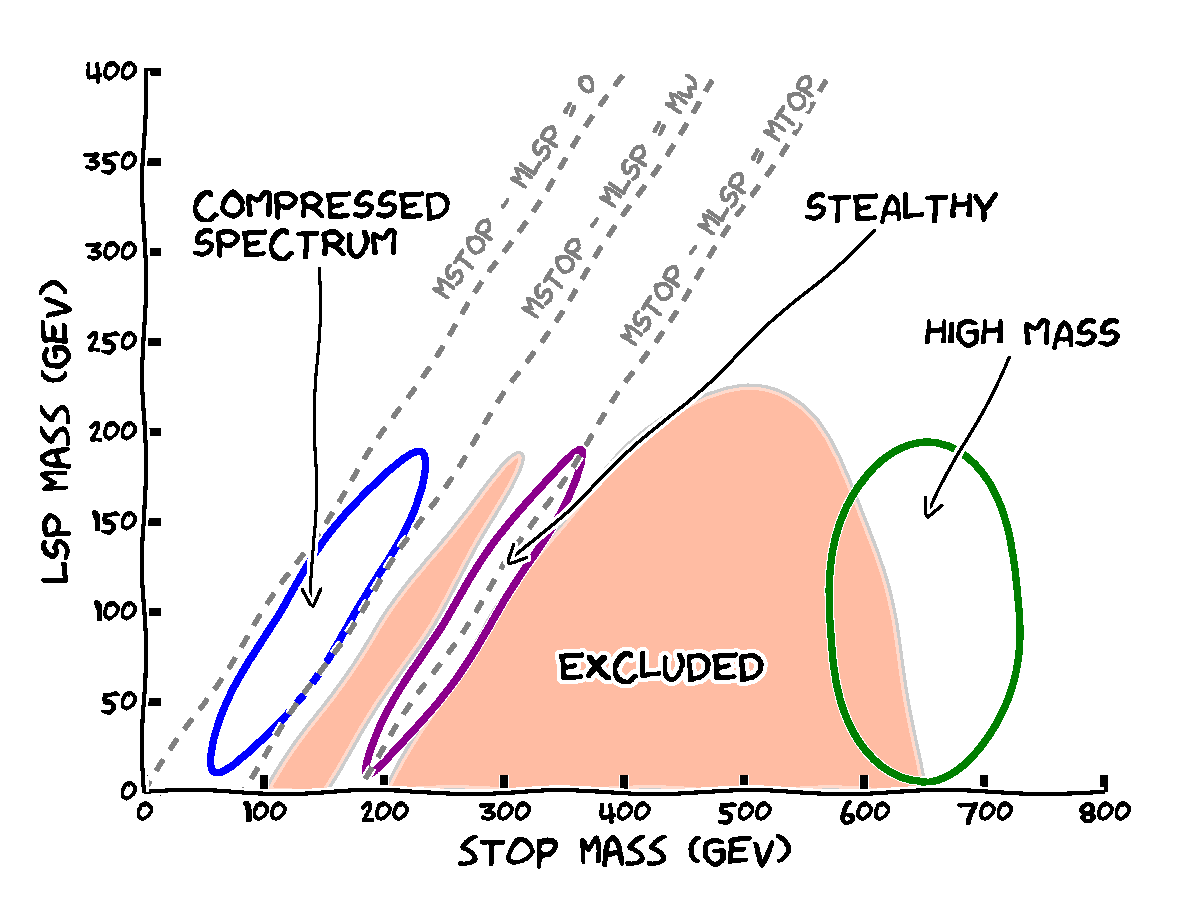
\includegraphics[width=0.8\textwidth]{figures/razor_motivation/story_boost_motivation}
  \caption{General form of the exclusion limits for direct stop production on the
($m_{\stopone},m_{\lsp}$) plane. The red shaded area is the approximate region that has been
excluded by a range of searches. The three colored ellipses indicate the regions that are hard to
probe: the compressed spectra, stealthy top squark scenario and high mass top squarks.
  \label{fig:boost_story_motivation}}
\end{figure}

\paragraph{Compressed scenario}
In general, models with mass spectra featuring small mass splittings are called \textit{compressed
scenarios} or \textit{compressed spectra}. This case thus corresponds to the left-most gap in
Fig.~\ref{fig:boost_story_motivation}, where $\Delta m$ is very small, smaller than the $\W$ boson
mass in particular. 
In this scenario, the top squark decays to the LSP and other soft decay products, either resulting
from the loop-induced decay $\stopone \rightarrow c \lsp$, or from the four-body decay $\stopone
\rightarrow \cPqb f \bar{f} \lsp$. These soft decay products, jets and/or leptons, are difficult to
detect. They are hard to reconstruct, and when reconstructed they often fall below the \pt
thresholds that define the objects. 
Therefore, in order to be sensitive to such processes, one should not rely on the presence of
these objects, but rather on something else, such as the presence of jets from initial state
radiation (ISR). Both ATLAS and CMS have performed searches using this
technique~\cite{CMS-PAS-SUS-13-009,Aad:2014nra}. 

\paragraph{Stealthy stop scenario}
The scenarios where $\Delta m\,{\approx}\, m_t$, are often referred to as \textit{stealthy}
scenarios. The reason for this is that when $\Delta m$ approaches the top mass, the signature of
top squark production is very similar to that of standard model $t\bar{t}$ production,
which has a much higher cross section. Consequently, the signal from direct stop production is
hidden underneath a much larger $t\bar{t}$ background. An alternate way to approach stealthy stops
is, for instance, to assume that the heavy top squark $\stoptwo$ is also accessible at the LHC, and
decays to the $\stopone$ via either a Higgs or $\cPZ$ boson~\cite{Khachatryan:2014doa}. This
results in a longer decay chain, which provides extra handles, such as additional $\cPqb$ quarks or
leptons. 

\paragraph{High mass scenario}
The last gap that is present in the sensitivity of searches for the direct production of top squark
pairs, is the high mass region. In this region the signature is actually very striking, with
usually large hadronic activity and/or missing transverse momentum. The problem lies in the rather
low expected cross section for direct stop production at 8\TeV. We would need much more data than
the $20\fbinv$ that is available to detect this process. 
Of course, with the restart of the LHC at 13\TeV centre-of-mass energy fast approaching, we can
expect to close part of this gap very soon.

\paragraph{}
Apart from the approaches mentioned above, there is another option to tackle the compressed and
stealthy scenarios, namely, looking for top squarks in gluino decays. This is exactly the focus of
the razor boost analysis. 
Specifically, we consider gluino pair production in which the gluino decays to a top squark and a
top quark, $\tilde{g} \rightarrow t \stopone$. In the models considered, largely motivated by
natural supersymmetry, the gluino has a mass around 1-1.5 \TeV and the lighter top squark has a mass
of a few hundred \GeV. Owing to the significant mass gap presumed to exist between the gluino and
the top squark, the top quark from the gluino to top squark decay will receive a large boost.  
The top squark then decays to $c \lsp$ for small $\Delta m$, or to $t \lsp$ for $\Delta m
\,{\approx}\, m_t$. Four-body decays of the top squark are not considered here. 

The simplified models (see Section~\ref{sec:susy_sms} for more information) corresponding to the
decays $\tilde{g} \rightarrow t \stopone$, followed by either $\stopone \rightarrow c \lsp$ or
$\stopone \rightarrow t \lsp$, are called \textit{T1ttcc} and \textit{T1t1t}, respectively, and
illustrated in the diagrams in Fig.~\ref{fig:T1ttcc_T1t1t_diagrams}. For comparison we show in
Fig.~\ref{fig:T2tt_diagram} the diagram for the \textit{T2tt} simplified model, corresponding to
direct top squark production in which the top squark decays to $t \lsp$. 

As the analysis described in this thesis is the first analysis within CMS to explicitely probe
gluino-mediated production of top squark pairs decaying as $\stopone \rightarrow c \lsp$, it
provides new information about the viability of natural SUSY. 

\begin{figure}
  \centering
  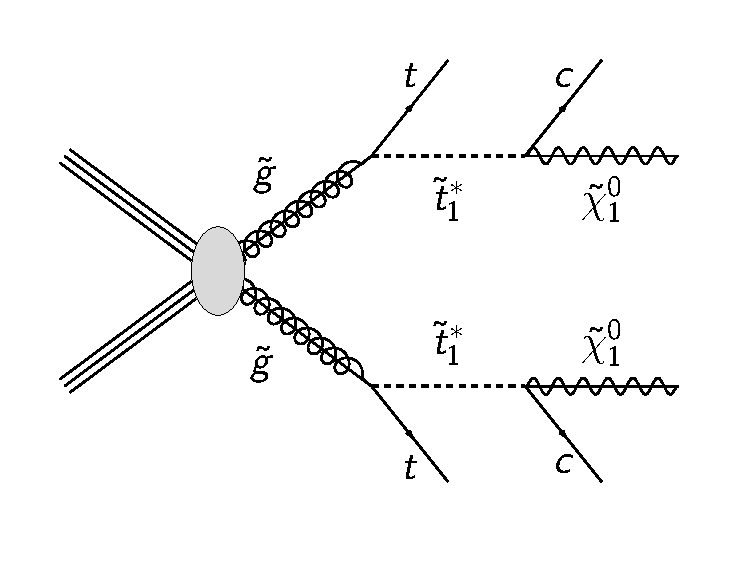
\includegraphics[width=0.48\textwidth,clip=true,trim=0 0.7cm 0 0]
{figures/razor_interpretation/T1ttcc}
  ~
  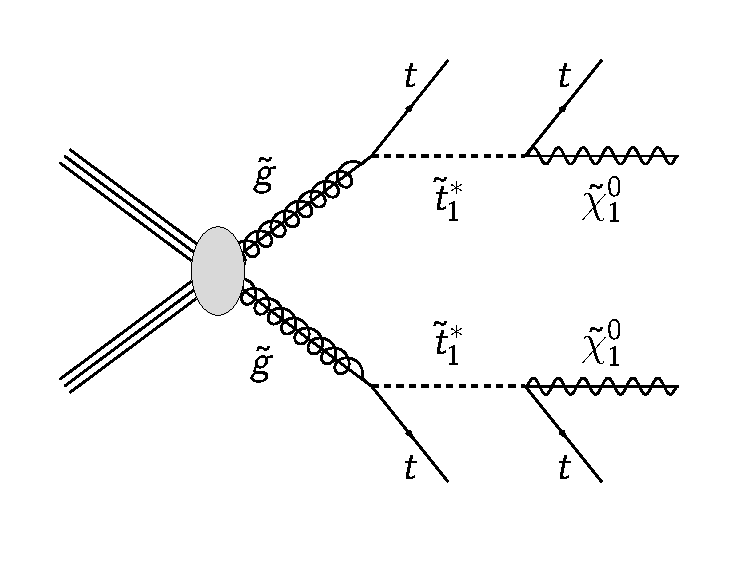
\includegraphics[width=0.48\textwidth,clip=true,trim=0 0.7cm 0 0]
{figures/razor_interpretation/T1t1t}
  \caption{Diagram illustrating the T1ttcc (left) and T1t1t (right) simplified models.
  \label{fig:T1ttcc_T1t1t_diagrams}}
\end{figure}

\begin{figure}
  \centering
  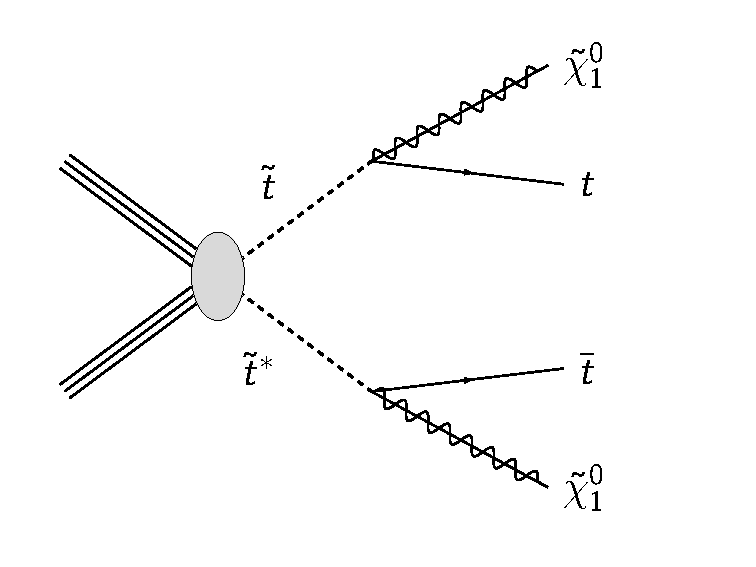
\includegraphics[width=0.48\textwidth,clip=true,trim=0 0.7cm 0 0]{figures/razor_motivation/T2tt}
  \caption{Diagram illustrating the T2tt simplified model.
  \label{fig:T2tt_diagram}}
\end{figure}




\section{General strategy \label{sec:boost_strategy}}

% control regions, transfer factors
% binning in razor variables
% statistical treatment and systematic uncertainties


In light of the discussion in Section~\ref{sec:boost_motivation}, it is expected that boosted top
quarks are a promising signature of new physics involving a massive gluino decaying to a relatively
light top squark.
Boosted objects with high transverse momentum are characterized by merged decay products
separated by $ \Delta R \,{\sim}\, 2m/\pt$\footnote{Considering a heavy object $\W$ with mass $M$
that decays to two massless particles $a$ and $b$, we find $M^2 = 2 p_a \cdot p_b = 2 E_a E_b (1
- \cos{\theta_{ab}})$. Using small angle approximation this becomes $M^2 = E_a E_b
\theta_{ab}^2$. Assigning half of the $\W$ energy to both $a$ and $b$ results in $M^2 =
\frac{1}{4} E_\W^2 \theta_{ab}^2$. Translating this relation into the transverse plane, we get
$\Delta R = \frac{2 M}{\pt^\W}$.}, 
where $m$ and $\pt$ denote the mass and transverse momentum of the mother particle, and $\Delta R$
is given in terms of azimuthal angle $\phi$ and pseudorapidity $\eta$ as $\Delta R = \sqrt{\Delta
\phi^2 + \Delta \eta^2}$.
For a separation of $\Delta R = 0.5$, a top quark should thus have a momentum of ${\sim}700$\GeV, a
value difficult to reach with proton-proton collisions at 8 TeV. Therefore, in order to increase the
signal efficiency, we consider instead $\W$ bosons from top quark decays, which are required to have
a more accessible $\pt \,{\sim}\, 320$\GeV.  The \pt of the top quark and $\W$ boson at generator
level without applying any selection, is shown in Figs.~\ref{fig:boost_gen_toppt} and
\ref{fig:boost_gen_Wpt} for several signal models, and the SM $t\bar{t}$ process. 
We observe that the average \pt is higher for the signal than for $t\bar{t}$. Requiring the
presence of a boosted $\W$ boson will thus be part of the strategy to reduce the SM background.
Hadronically decaying boosted $\W$ boson candidates will be identified using pruned jet
mass~\cite{Ellis:2009su,Ellis:2009me,Chatrchyan:2013vbb} and a jet substructure observable
called N-subjettiness \cite{Thaler:2010tr}. More details on the $\W$ tagging technique will be given
in Section~\ref{sec:boost_wtag}. 

\begin{figure}[htpb]
\centering
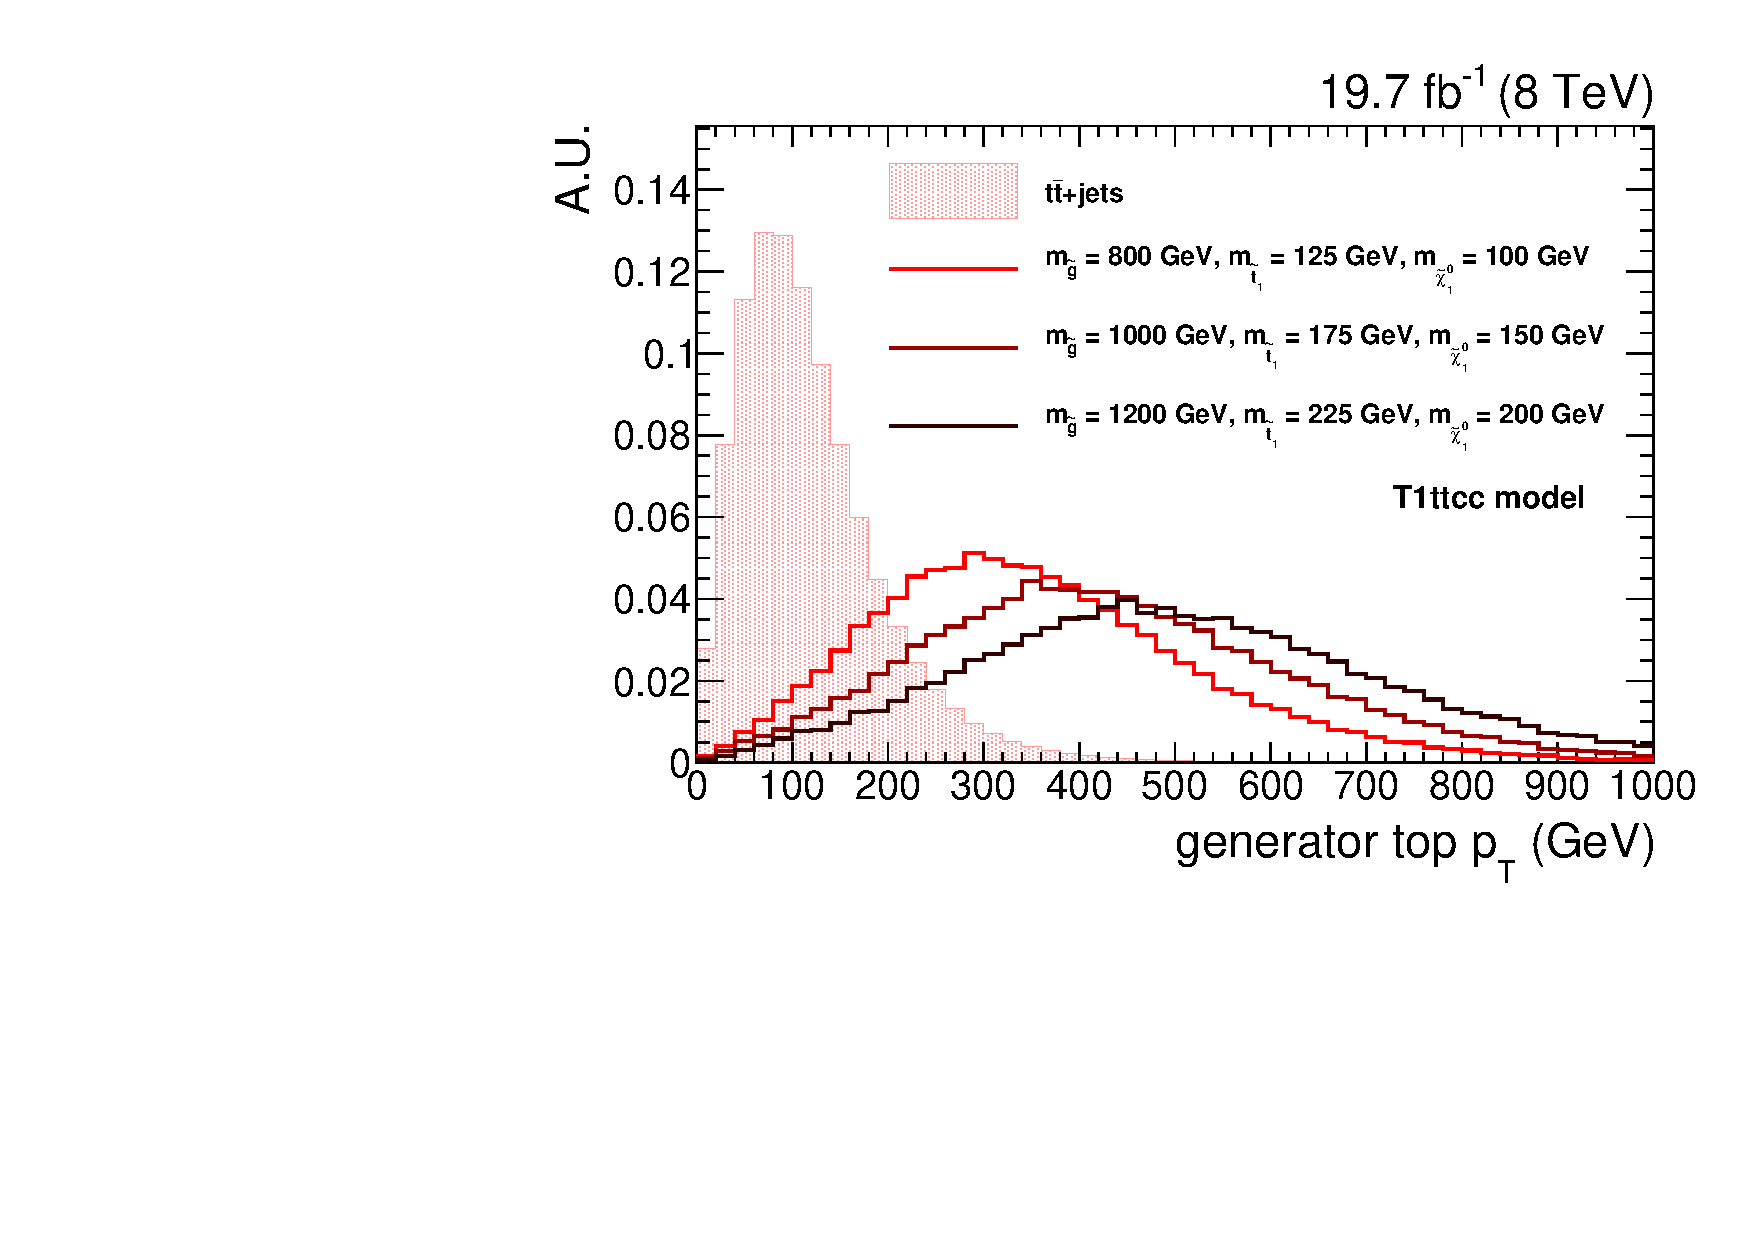
\includegraphics[width=0.48\textwidth]{figures/razor_strategy/T1ttcc_gentoppt}
~
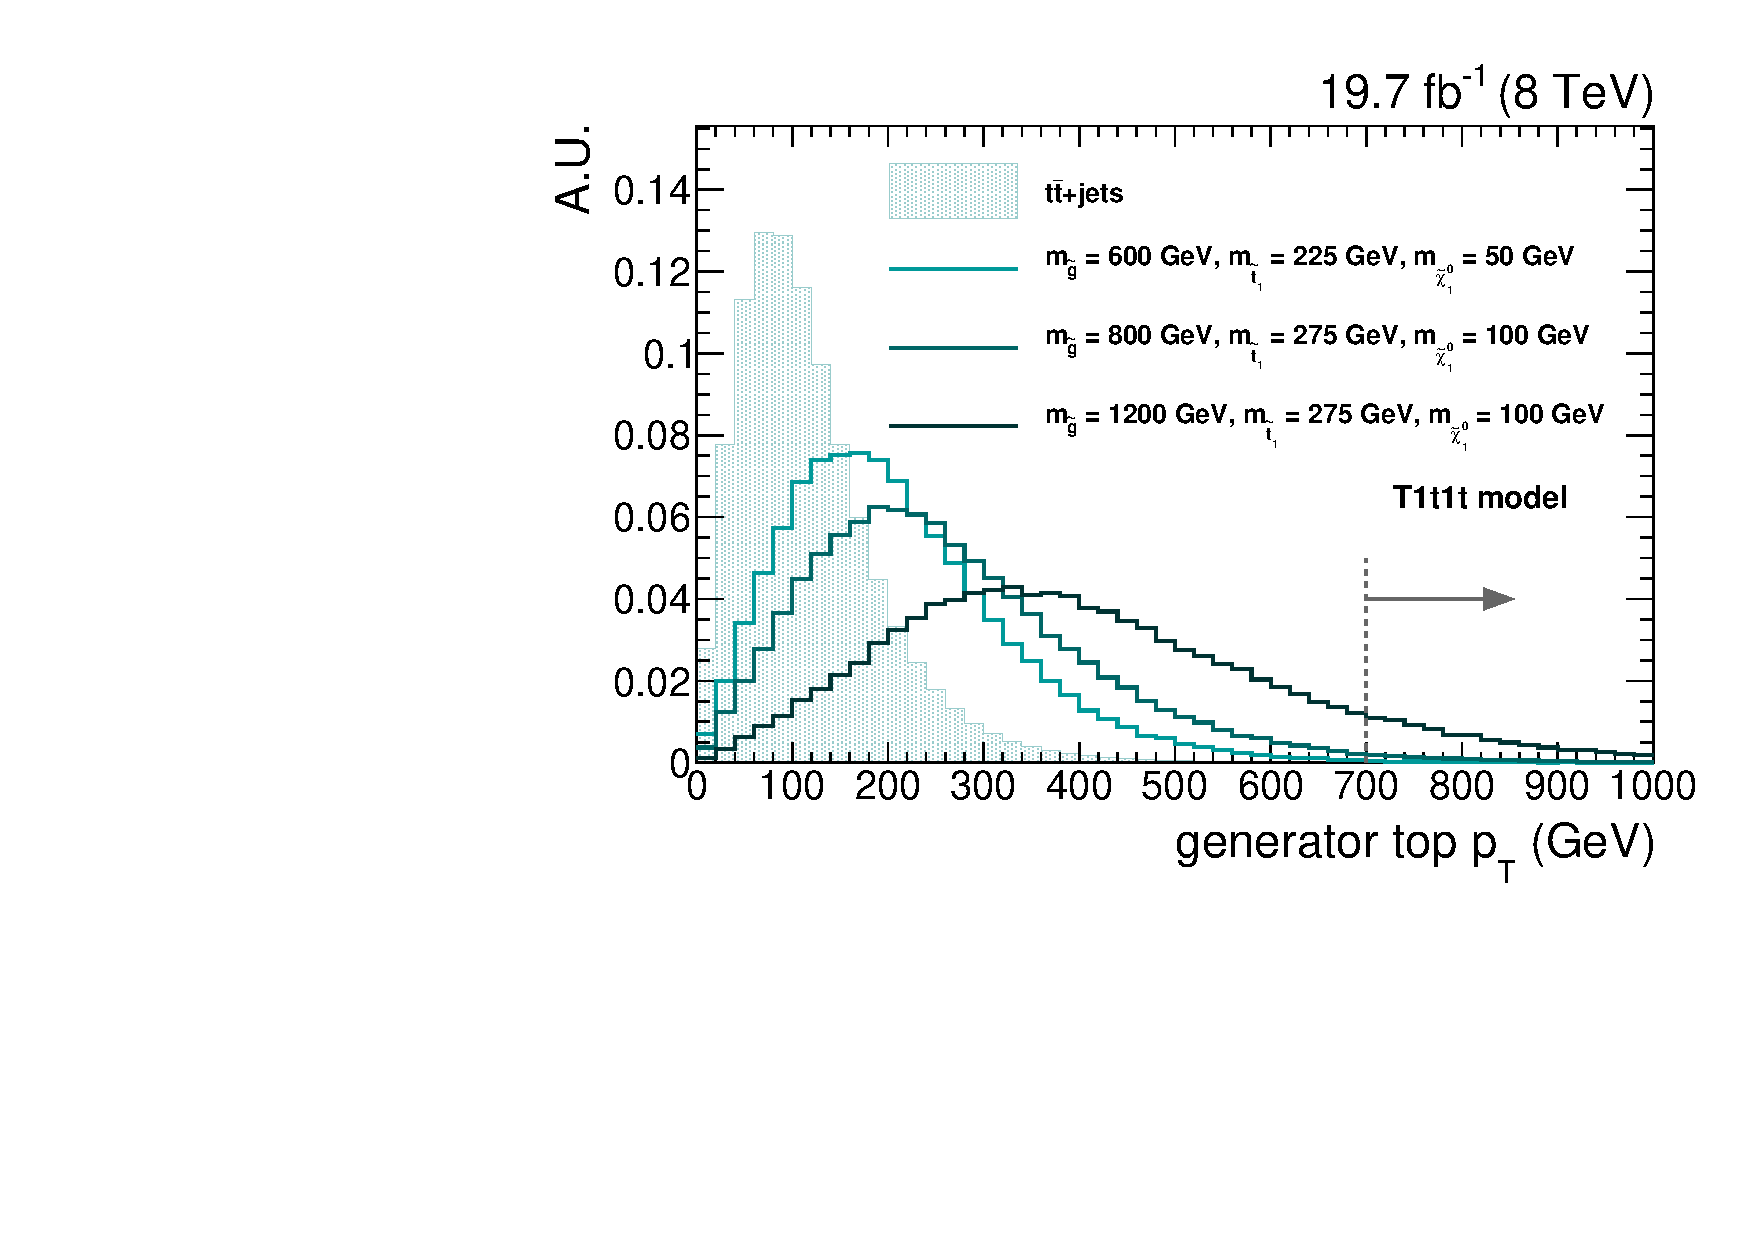
\includegraphics[width=0.48\textwidth]{figures/razor_strategy/T1t1t_gentoppt}
\caption{Generator level top quark \pt for several signal points of the T1ttcc (left) and T1t1t
(right) simplified models. The average \pt increases as the mass splitting increases. The boost of
the top quark is larger for the considered signal models compared to the $t\bar{t}$ background. 
\label{fig:boost_gen_toppt}}
\end{figure}
\begin{figure}[htpb]
\centering
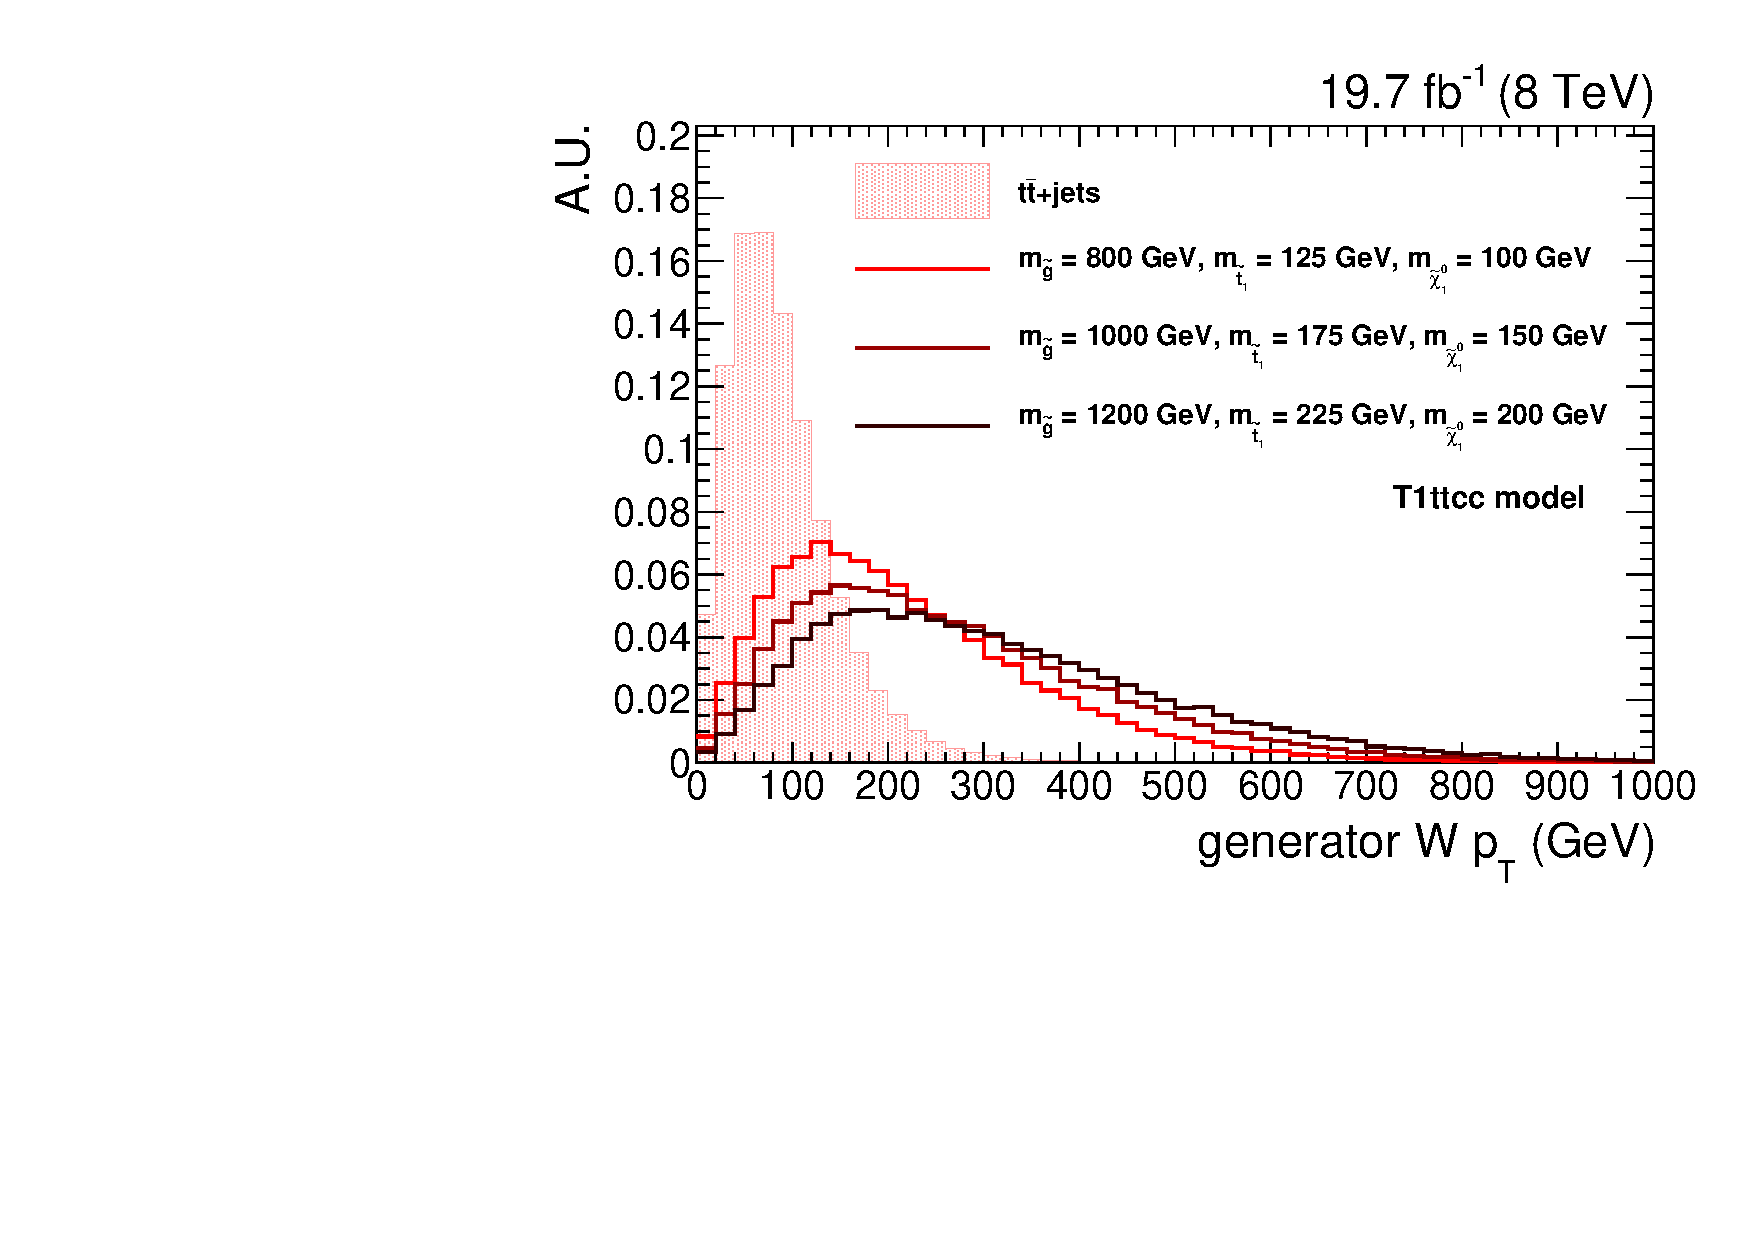
\includegraphics[width=0.48\textwidth]{figures/razor_strategy/T1ttcc_genWpt}
~
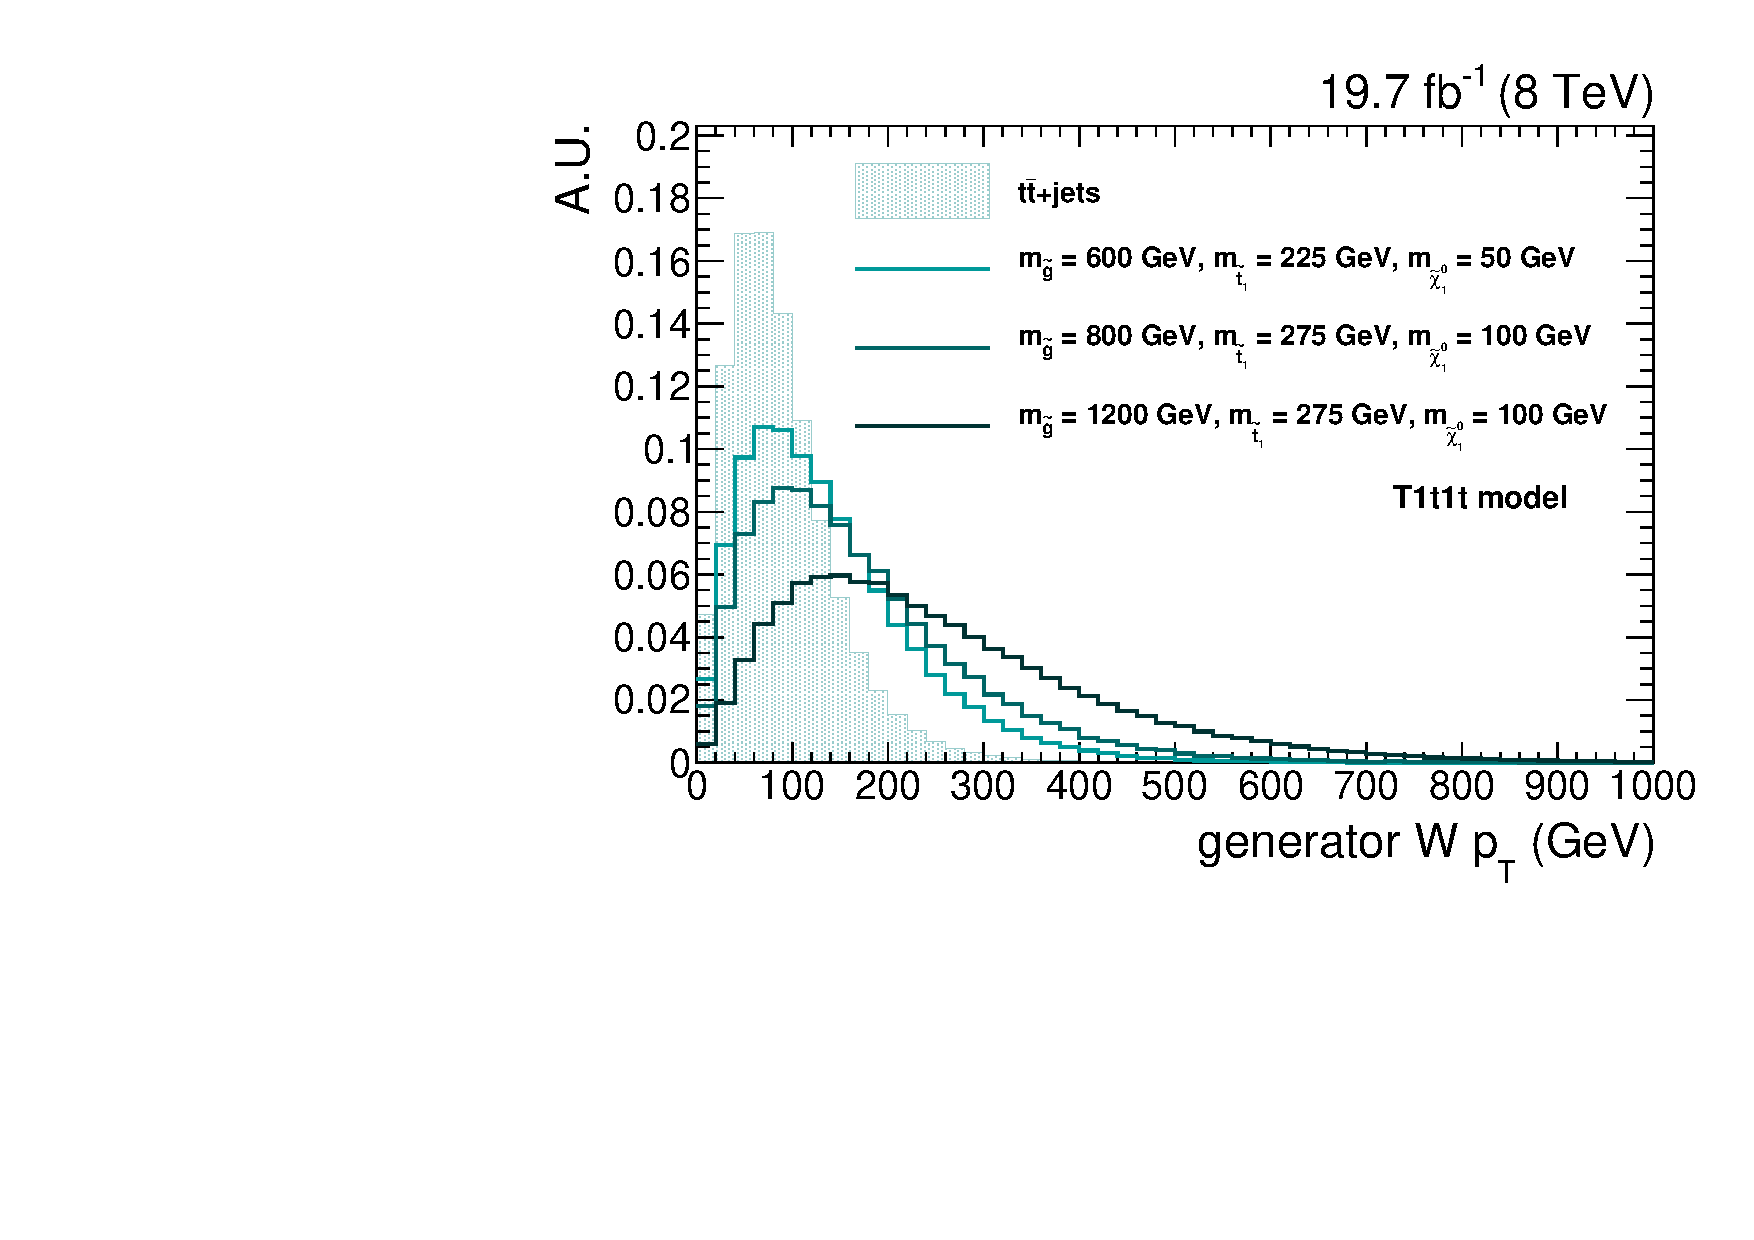
\includegraphics[width=0.48\textwidth]{figures/razor_strategy/T1t1t_genWpt}
\caption{Generator level $\W$ boson \pt for several signal points of the T1ttcc (left) and T1t1t
(right)
simplified models. The average \pt increases as the mass splitting increases. The boost of the $\W$
boson is larger for the considered signal models compared to the $t\bar{t}$ background. 
\label{fig:boost_gen_Wpt}}
\end{figure}

The razor kinematic variables \mr and \rsq, see Section~\ref{sec:boost_razor}, are designed to
discriminate processes with new heavy particles and missing energy from standard model processes.
They will be used in this analysis as the main discriminating variables to search for deviations
from the SM. We will perform the search in 25 search bins across the high $\mr$-high $\rsq$ region,
using hadronic events with at least one boosted $\W$ boson and one jet originating from a $\cPqb$
quark (i.e. $\cPqb$ jet). 

Standard model backgrounds in the signal regions are estimated using observations in control regions
and global scale factors, calculated from simulated data, that relate the number of events in one
region to that in another. 
Three control regions, $Q$, $W$, and $T$, are defined to select high-purity samples of multijet,
$\W(\rightarrow \ell\nu)+$jets and $t\bar{t}$ processes, respectively.  
The background estimation method uses a likelihood-based approach, with a simultaneous sampling
of systematic uncertainties which fully takes into account any correlations automatically.
An overview of the different regions and how they are related, including for the control regions
which background parameters of the likelihood each region constrains, is shown in
Fig.~\ref{fig:boost_flowchart}. For the full explanation of the background estimation method, I
refer to Section~\ref{sec:boost_likelihood}. 

\begin{figure}[p]
  \centering
  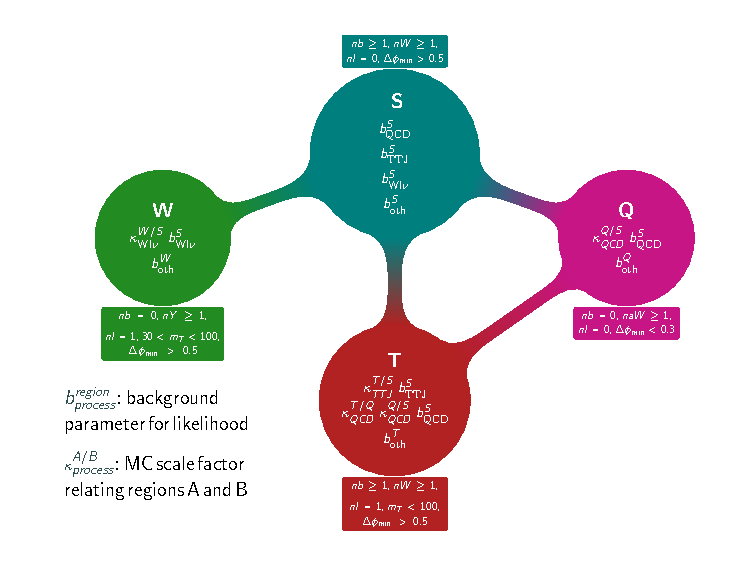
\includegraphics[width=\textwidth]{figures/razor_strategy/BoostFlowChart_noZ}
  \caption{Definition of, and relationship between, the signal ($S$) and control ($Q,T,W$) regions
and their relationship to the bin-by-bin background parameters
$b^{\textrm{region}}_{\textrm{process}}$ for a given region and background process, as well as the
four global scale factors $\kappa^{A/B}_{\textrm{process}} = \sum_i b^A_{\textrm{process}, MC, i} /
\sum_i b^B_{\textrm{process}, MC, i}$, where the sum is over all 25 (\mr,\rsq) bins of the simulated
data. 
The total expected background, per bin, is the sum of the terms shown for each region. Furthermore,
associated with each bin of each region is an observed count $N^{\textrm{region}}$, a simulated
count $N^{\textrm{region}}_{\textrm{process}, MC}$, and a count $N^{\textrm{region}}_{oth, MC}$
equal to the sum of the smaller backgrounds, with associated parameter $b^{\textrm{region}}_{oth}$.
  \label{fig:boost_flowchart}}
\end{figure}

% 
% \begin{figure}[htbp]
% \centering
% \includegraphics[width=0.49\textwidth]{figures/T1ttcc/Signal_comparison_T1ttcc_gen_toppt}
% \includegraphics[width=0.49\textwidth]{figures/T1t1t/Signal_comparison_T1t1t_gen_toppt}
% \caption{Generator top \pt for several signalpoints of the T1ttcc (left) andT1t1t (right)
% simplified
% models.
% \label{fig:gen_toppt}}
% \end{figure}

\section{Razor variables \label{sec:boost_razor}}

%%%%%%%%%%%%%%%%%%%
% razor variables
%%%%%%%%%%%%%%%%%%%

% add full derivation
% plots of signal and background

Many extensions of the Standard Model (see chapter~\ref{chap:beyond_standard_model}) predict the 
existence of new particles, which can be pair-produced in the proton-proton collisions at the LHC. 
Some of those theories introduce an extra symmetry, such as the R-parity in supersymmetry. A
consequence of this symmetry is that the lightest BSM particle must be stable, as it cannot decay
to SM particles only. This lightest BSM particle, called LSP in supersymmetric theories, is weakly
interacting, and escapes the detector unseen. 

This general property leads us to a generic class of new physics signatures in which a heavy
particle is pair-produced, and decays into visible, i.e. interacting with our detector, SM
particles, and an invisible LSP. This signature is illustrated in figure~\ref{fig:razor_signature}.

\begin{figure}[htb]
  \centering
  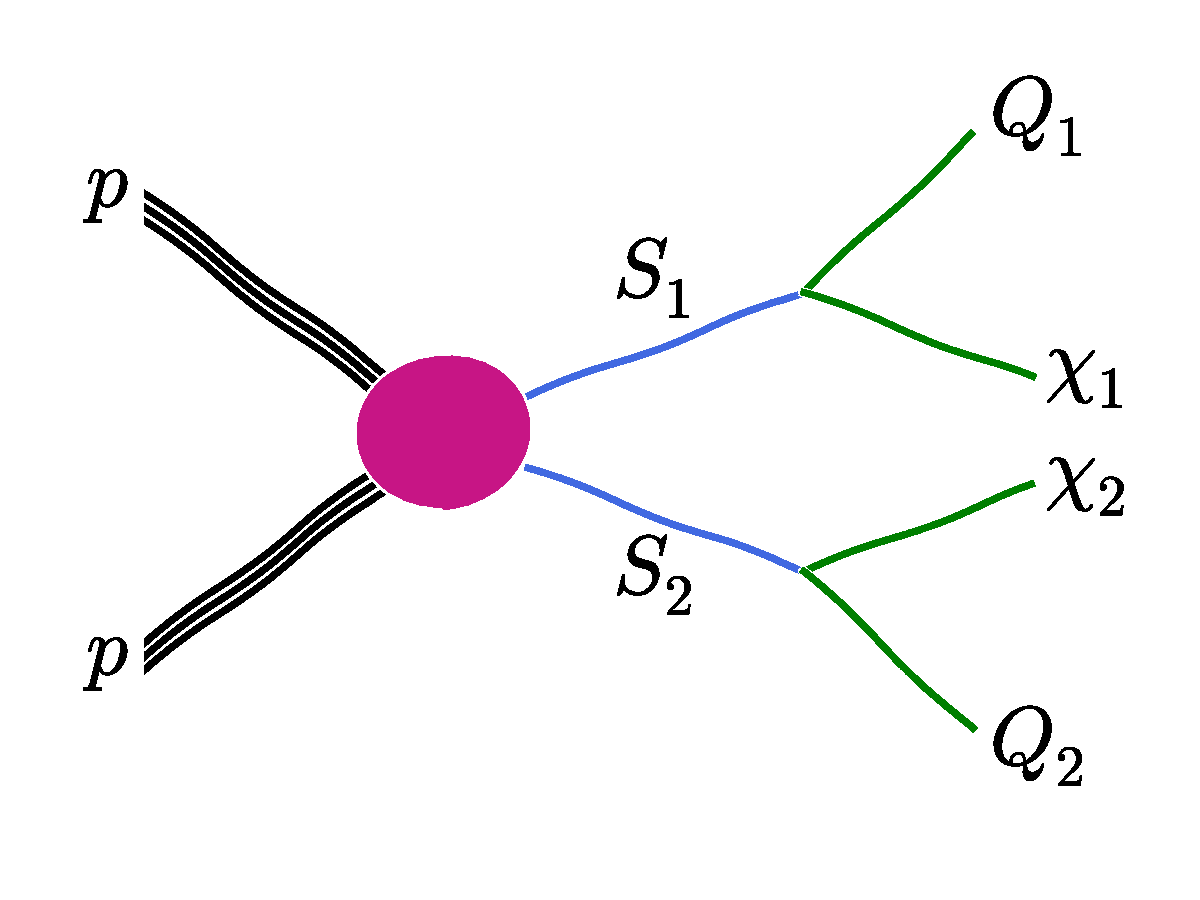
\includegraphics[width=0.6\textwidth,clip=true,trim=0 1.8cm 0
0.8cm]{figures/razor_variables/signature} 
  \caption{Generic new physics signature. Two massive new particles, $S_1$ and $S_2$, are produced
in $\Pp\Pp$ collisions at the LHC, and consequently decay to a visible system $Q_i$ and an invisible
system $\chi_i$. \label{fig:razor_signature}}
\end{figure}

Several kinematical variables targetting this topology have been
developed~\cite{Lester:1999tx,Barr:2003rg,Randall:2008rw,Polesello:2009rn,Bai:2012gs}.
% TODO add citations here
Most of these variables rely on the presence of the invisible LSP's. This causes the visible system
to deviate from a di-jet topology, resulting in possibly large missing transverse momentum, altered
angular distributions, et cetera. All of this can be used to distinguish the sought-after signal
from the known background processes. 
Unfortunately, the ultimate goal of reconstructing the masses of the new particles cannot be
attained. Because of the escaping LSP's, there is simply not enough information available to fully
constrain the problem. What we can do, however, is approximate the mass scale of the new physics
particles. Often times this results in variables that exhibit a kinematic edge. 
The \textit{razor variables} \cite{rogan,Rogan:1557072,Chatrchyan:2011ek,Chatrchyan:2014goa} are no
exception in this regard. One advantage the razor variables have over many other variables, is that
they also reconstruct the mass scale as a peak, in addition to a kinematic edge. 
In what follows I will derive the two razor variables, denoted \mr and \rsq, which use longitudinal
and transverse event information, respectively, to estimate a characteristic mass scale associated
with the new particles. At the end of this section I will briefly show how the razor variables are
used in the razor boost analysis. 

% explain reference frames

\subsection{Kinematical configuration and notation \label{sec:razor_notation}}

Let's again consider figure~\ref{fig:razor_signature}. For simplicity, we will assume that the
produced particles $S_1$ and $S_2$ undergo a two-body decay. Each $S_i$ decays to a visible,
standard model particle $Q_i$, and a particle $\chi_i$ that escapes the detector. 
We assume a symmetric decay chain, with the following relations for the masses of the different
particles,
\begin{alignat}{3}
  M_{S_1} &= M_{S_2} &&= M_S \label{eq:equal_S_masses}\\
  M_{\chi_1} &= M_{\chi_2} &&= M_{\chi} \label{eq:equal_chi_masses}\\
  M_{Q_1} &= M_{Q_2} &&= 0 \label{eq:no_Q_masses}
\end{alignat}

There are four relevant reference frames for our goal of determining a characteristic mass scale
of the new physics process under consideration. The following paragraphs will go through each of
these and define the notations that will be used, as well as deriving relations between several
variables. 

\paragraph{$S_1$ rest frame} 
From basic two-body decay kinematics it follows that the $Q_1$ and $\chi_1$ particles are produced
back to back, with equal magnitude of momentum, in the rest frame of the $S_1$ particle. This is
illustrated in figure~\ref{fig:razor_S1_rest_frame}. 

\begin{figure}[htpb]
  \centering
  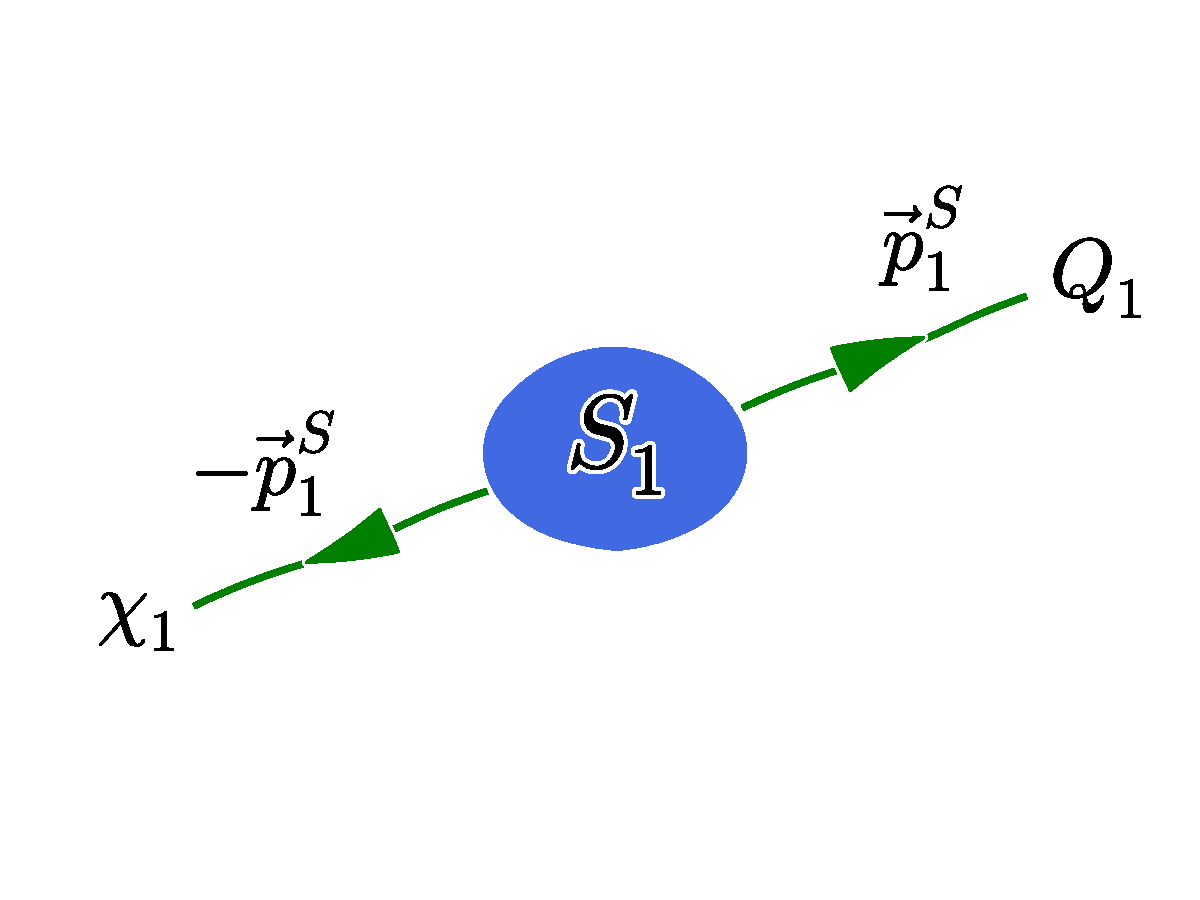
\includegraphics[width=0.6\textwidth,clip=true,trim=0 4cm 0
3cm]{figures/razor_variables/rest_frame}
  \caption{Configuration of the $S_1$ rest frame. The decay products $Q_1$ and $\chi_1$ are
produced back to back with momenta $\vec{p}^S_1$ and $-\vec{p}^S_1$, respectively. 
\label{fig:razor_S1_rest_frame}}
\end{figure}

We can compute the magnitude of this momentum in terms of the new particle masses. To do this we
start from the four-vectors of the $Q_1$ and $\chi_1$ particles in the $S_1$ rest frame, 
\begin{alignat}{6}
  P[Q_1]    &\equiv q_1^S   &&= \{ E^S_{Q_1}, \vec{q}^S_1\} , \\
  P[\chi_1] &\equiv \nu_1^S &&= \{ E^S_{\chi_1}, \vec{\nu}^S_1\} .
\end{alignat}
Conservation of energy in the $S_1$ rest frame leads to 
\begin{equation}
  E^S_{Q_1} + E^S_{\chi_1} = M_S . \label{eq:razor_conservation_energy}
\end{equation}
This can also be expressed as
\begin{equation}
  \sqrt{M_{Q_1}^2 + (\vec{q}^S_1)^2 } + \sqrt{M_{\chi_1}^2 + (\vec{\nu}^S_1)^2} = M_S .
\end{equation}
Using Eq.~\ref{eq:equal_chi_masses} and Eq.~\ref{eq:no_Q_masses} (massless $Q_1$), and the equal
momenta $|\vec{q}^S_1| = |\vec{\nu}^S_1| = |\vec{p}^S_1|$, the above can be simplified as
\begin{align}
  |\vec{p}^S_1|   &= M_S - \sqrt{M_{\chi}^2 + (\vec{p}^S_1)^2} \\
  (\vec{p}^S_1)^2 &= M_S^2 - 2 M_S \sqrt{M_{\chi}^2 + (\vec{p}^S_1)^2} + M_{\chi}^2 +
(\vec{p}^S_1)^2 \\
  2 M_S \sqrt{M_{\chi}^2 + (\vec{p}^S_1)^2} &= M_S^2 + M_{\chi}^2 \\
  4 M_S^2 (\vec{p}^S_1)^2 &= (M_S^2)^2 + 2 M_S^2 M_{\chi}^2 + (M_{\chi}^2)^2 - 4 M_S^2
M_{\chi}^2 \\
  (\vec{p}^S_1)^2 &= \frac{(M_S^2 -M_{\chi}^2 )^2}{4 M_S^2} .
\end{align}

We thus find for the magnitude of the momentum of $Q_1$ and $\chi_1$ in the $S_1$ rest frame
\begin{equation}
  |\vec{p}^S_1| = \frac{M_S^2 -M_{\chi}^2}{2 M_S} \equiv \frac{M_\Delta}{2} ,
\label{eq:razor_p_S1_rest_frame}
\end{equation}
where we have defined the characteristic scale $M_\Delta$. This scale is exactly the scale we are
interested in. The goal of the \textbf{razor variables} is to \textbf{express $M_\Delta$ using lab
frame quantities only}. To succeed in this effort, we will have to make several, physics-motivated,
approximations. These will remove the unknown degrees of freedom, and are further explained in
sections~\ref{sec:razor_mr} and \ref{sec:razor_r2}. 

The energy of the $Q_1$ and $\chi_1$ particles can also be computed easily. 
From the masslessness of $Q_1$, we immediately find using Eq.~\ref{eq:razor_p_S1_rest_frame}
\begin{equation}
  E^S_{Q_1} = |\vec{p}^S_1| = \frac{M_\Delta}{2}. \label{eq:razor_E_Q1}
\end{equation}
To compute $E^S_{\chi_1}$, we substitute Eq.~\ref{eq:razor_E_Q1} in 
Eq.~\ref{eq:razor_conservation_energy}, and find 
\begin{align}
  E^S_{\chi_1} &= M_S - |\vec{p}^S_1|\\
	       &= M_S - \frac{M_S^2 -M_{\chi}^2}{2 M_S} \\
	       &= \frac{2M_S^2 - M_S^2 + M_{\chi}^2}{2 M_S} \\
	       &= \frac{M_S^2 + M_{\chi}^2}{2 M_S} \\
	       &= \frac{M_S^2 - M_{\chi}^2}{2 M_S} \frac{M_S^2 + M_{\chi}^2}{M_S^2 - M_{\chi}^2} .
%               &= \frac{M_\Delta}{2} R_{S\chi}
\end{align}

We can summarize the four-momenta of $Q_1$ and $\chi_1$ in the $S_1$ rest frame as
\begin{align}
  q_1^S   &= \frac{M_\Delta}{2} \{ 1, \vec{u}_1\} , \\  
  \nu_1^S &= \frac{M_\Delta}{2} \{ R_{S\chi}, -\vec{u}_1\} ,
\end{align}
with $$R_{S\chi} = \frac{M_S^2 + M_{\chi}^2}{M_S^2 - M_{\chi}^2},$$ and $\vec{u}_1$ the unit
vector along the $Q_1$ momentum direction.



\paragraph{$S_2$ rest frame}
The discussion of the $S_2$ rest frame is fully analogous to that of the $S_1$ rest frame. We
again find that
\begin{align}
  q_2^S   &= \frac{M_\Delta}{2} \{ 1, \vec{u}_2\} , \\  
  \nu_2^S &= \frac{M_\Delta}{2} \{ R_{S\chi}, -\vec{u}_2\} ,
\end{align}
and thus
\begin{equation}
  |\vec{p}^S_1| = |\vec{p}^S_2| = \frac{M_\Delta}{2} . \label{eq:razor_equal_momenta}
\end{equation}


\paragraph{Center-of-mass frame}
In the center-of-mass (CM) frame of the considered $\Pp\Pp$ collision events the particles $S_1$
and $S_2$, which have equal mass (Eq.~\ref{eq:equal_S_masses}), are produced with equal and opposite
velocities $\betaCM$, as illustrated in figure~\ref{fig:razor_CM_frame}. The boost $\betaCM$ is an
indication of how far above threshold the $S_i$ particles are produced, but unfortunately this is
an unknown at hadron colliders. 

\begin{figure}[htpb]
  \centering
  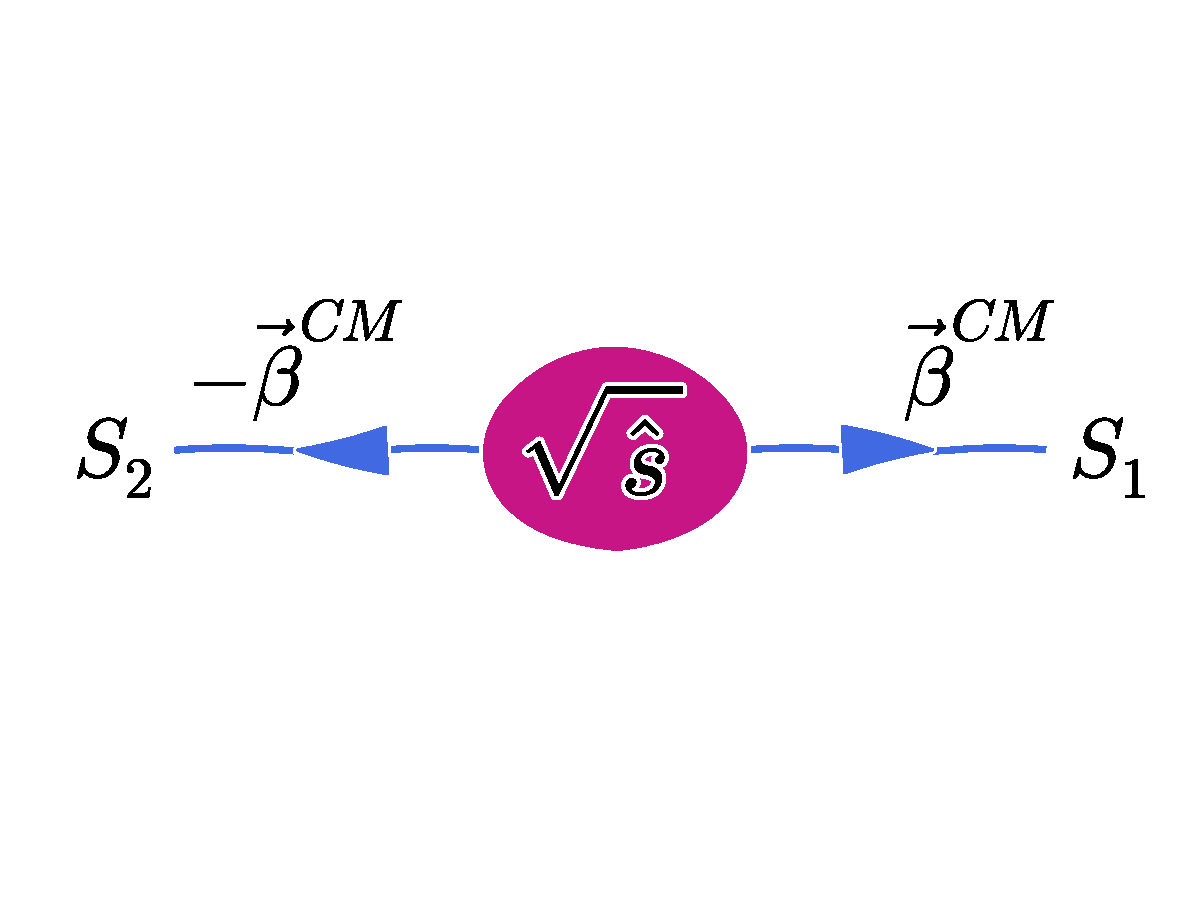
\includegraphics[width=0.6\textwidth,clip=true,trim=0 5.5cm 0
4.5cm]{figures/razor_variables/cm_frame} 
  \caption{Configuration of the center-of-mass frame. The particles $S_1$ and $S_2$ are
produced back to back with velocities $\betaCM$ and $-\betaCM$, respectively. 
\label{fig:razor_CM_frame}}
\end{figure}

To go from the rest frame of $S_1$ ($S_2$) to the CM frame, we need to boost the four-momenta
$q_1^S$ and $\nu_1^S$ ($q_2^S$ and $\nu_2^S$) to the frame travelling at velocity $\betaCM$
($-\betaCM$) with respect to the $S_1$ ($S_2$) rest frame. 
The four-vectors of particles $S_1$ and $S_2$ in the center-of-mass frame are also obtained by
boosting according to $\betaCM$. They can be written as
\begin{alignat}{6}
  P[S_1] &\equiv s^{\textrm{CM}}_1  &&= \{ E^{\textrm{CM}}_{S_1} , \vec{s}^{\textrm{CM}}_{S_1}\} 
&&= M_S \, \gamma^{\textrm{CM}} \, \{ 1 , \betaCM\} , \\ 
  P[S_2] &\equiv s^{\textrm{CM}}_2 &&= \{ E^{\textrm{CM}}_{S_2} , \vec{s}\,^{\textrm{CM}}_{S_2}\}
&&= M_S \, \gamma^{\textrm{CM}} \, \{ 1 , -\betaCM\},  
\end{alignat}
and satisfy the following
\begin{equation}
  (s^{\textrm{CM}}_1 + s^{\textrm{CM}}_1)^2 = \hat{s} = 4 (\gamma^{\textrm{CM}})^2 M_S^2,
\end{equation}
with $\sqrt{\hat{s}}$ the center-of-mass energy of the collision. 


\paragraph{Lab frame}
The lab frame is the frame where we make our measurements, and is related to the CM frame by a
boost $\vec{\beta}^{\textrm{lab}}$. We can decompose this boost into a transverse and longitudinal
part as $\vec{\beta}^{\textrm{lab}} = (\vec{\beta}_T,\vec{\beta}_z)$. 
The four-momenta of the $S_i$, $Q_i$ and $\chi_i$ particles are denoted by $s^{\textrm{lab}}_i$,
$q^{\textrm{lab}}_i$, and $\nu^{\textrm{lab}}_i$ respectively. 



\subsection{Derivation of \texorpdfstring{\mr}{MR} \label{sec:razor_mr}}

As mentioned in the previous section, our goal is to express the characteristic scale $M_\Delta$
using lab frame quantities only. Because the problem is kinematically underconstrained, we will
need to make some approximations as we work our way from the lab frame to the $S_i$ rest frame,
reversing the boosts $\vec{\beta}^{\textrm{lab}}$ and $\betaCM$ as we go along. 

The models of new physics that we aim to target with the razor variables all predict that the new
particles are heavy. This prediction is the basis of the two approximations we will be making. 

\begin{enumerate}
  \item If $M_S$ is large compared to $\sqrt{s}$, then the particles $S_1$ and $S_2$ will be
produced near the $\sqrt{\hat{s}} = 2 M_S$ threshold. This means that $\gamma^{\textrm{CM}} \approx
1$. We will thus assume that $\gamma^{\textrm{CM}} = 1$, which means that $\betaCM \rightarrow 0$. 
The CM frame is thus equal to both $S_i$ rest frames after this first approximation. 
  \item The transverse boost between lab frame and CM frame can be approximated by 
  \begin{equation}
    |\vec{\beta}_T| \approx \frac{p_T^{ISR}}{\sqrt{\hat{s}}} \lesssim \frac{p_T^{ISR}}{2M_S},
  \end{equation}
  where $p_T^{ISR}$ is the magnitude of the vectorial sum of the transverse momentum of the initial
state radiation. For large values of $M_S$ we find $\vec{\beta}_T \ll 1$. We thus assume that
$\vec{\beta}_T \rightarrow 0$, and thus $\vec{\beta}^{\textrm{lab}} \rightarrow \vec{\beta}_z$.
\end{enumerate}
The results of these two approximations is that we only need a longitudinal boost $\vec{\beta}_z$
to take us from the lab frame to the approximate $S_i$ rest frames. 
In this so-called \textit{rough-approximation frame}, or \textit{R-frame}, we have that
\begin{alignat}{4}
  |\vec{q}^R_1|         &= |\vec{q}^R_2| &&= \frac{M_\Delta}{2} , \\
  \textrm{or } E_{Q_1}^R &= E_{Q_2}^R     &&= \frac{M_\Delta}{2}.
\label{eq:razor_equal_energy_R_frame}
\end{alignat}
cf. Eq.~\ref{eq:razor_equal_momenta}. Using this constraint, we can compute the boost $\beta^R$
that will take us from the lab frame to the R-frame. We start from the basic Lorentz
transformations for energy and momentum, 
\begin{align}
  E_{Q_i}^R      &= \gamma^R \left( E_{Q_i}^{\textrm{lab}} - \beta^R \vec{q}_{iz}^{\textrm{lab}}
\right) , \\
  \vec{q}_{iz}^R &= \gamma^R \left( \vec{q}_{iz}^{\textrm{lab}} - \beta^R E_{Q_i}^{\textrm{lab}}
\right) .
\end{align}
Using Eq.~\ref{eq:razor_equal_energy_R_frame} we find
\begin{equation}
  E_{Q_1}^{\textrm{lab}} - \beta^R \vec{q}_{1z}^{\textrm{lab}} = E_{Q_2}^{\textrm{lab}} - \beta^R
\vec{q}_{2z}^{\textrm{lab}} ,
\end{equation}
and thus for the boost $\beta^R$
\begin{equation}
  \beta^R = \frac{E_{Q_1}^{\textrm{lab}} - E_{Q_2}^{\textrm{lab}}}{\vec{q}_{1z}^{\textrm{lab}} -
\vec{q}_{2z}^{\textrm{lab}}} . \label{eq:razor_beta_R}
\end{equation}
The Lorentz factor $\gamma^R$ can be expressed as
\begin{align}
  \gamma^R &= \frac{1}{\sqrt{1 - (\beta^R)^2}} \\
	   &= \frac{1}{\sqrt{1 - \left( \frac{E_{Q_1}^{\textrm{lab}} -
E_{Q_2}^{\textrm{lab}}}{\vec{q}_{1z}^{\textrm{lab}} -
\vec{q}_{2z}^{\textrm{lab}}} \right)^2}} \\
           &= \frac{ \vec{q}_{1z}^{\textrm{lab}} - \vec{q}_{2z}^{\textrm{lab}} }{\sqrt{ \left(
 \vec{q}_{1z}^{\textrm{lab}} - \vec{q}_{2z}^{\textrm{lab}} \right)^2 - \left(
 E_{Q_1}^{\textrm{lab}} - E_{Q_2}^{\textrm{lab}}\right)^2 }} \label{eq:razor_gamma_R}
\end{align}

We now define \mr as
\begin{equation}
  \mr \equiv 2 |\vec{q}^R| = M_\Delta .
\end{equation}
It is interesting to note that \mr is invariant under longitudinal boosts. Using
Eq.~\ref{eq:razor_beta_R} and Eq.~\ref{eq:razor_gamma_R}, we can express \mr using lab frame
quantities only. 

\begin{align}
  \mr &= E_{Q_1}^R + E_{Q_2}^R \\
      &= \gamma^R \left( E_{Q_1}^{\textrm{lab}} + E_{Q_2}^{\textrm{lab}} - \beta^R (
\vec{q}_{1z}^{\textrm{lab}} + \vec{q}_{2z}^{\textrm{lab}}) \right) \\
      &= \frac{\left( \vec{q}_{1z}^{\textrm{lab}} - \vec{q}_{2z}^{\textrm{lab}}\right) 
               \left( E_{Q_1}^{\textrm{lab}} + E_{Q_2}^{\textrm{lab}} - \frac{E_{Q_1}^{\textrm{lab}}
- E_{Q_2}^{\textrm{lab}}}{\vec{q}_{1z}^{\textrm{lab}} - \vec{q}_{2z}^{\textrm{lab}}}
(\vec{q}_{1z}^{\textrm{lab}} + \vec{q}_{2z}^{\textrm{lab}}) \right)}
              { \sqrt{ \left( \vec{q}_{1z}^{\textrm{lab}} - \vec{q}_{2z}^{\textrm{lab}} \right)^2 
                      -\left( E_{Q_1}^{\textrm{lab}} - E_{Q_2}^{\textrm{lab}}\right)^2 }} \\
      &= \frac{\left( \vec{q}_{1z}^{\textrm{lab}} - \vec{q}_{2z}^{\textrm{lab}} \right) 
               \left( E_{Q_1}^{\textrm{lab}} + E_{Q_2}^{\textrm{lab}} \right) 
               - 
               \left( E_{Q_1}^{\textrm{lab}} - E_{Q_2}^{\textrm{lab}} \right)
               \left( \vec{q}_{1z}^{\textrm{lab}} + \vec{q}_{2z}^{\textrm{lab}} \right) }
              { \sqrt{ \left( \vec{q}_{1z}^{\textrm{lab}} - \vec{q}_{2z}^{\textrm{lab}} \right)^2 
                      -\left( E_{Q_1}^{\textrm{lab}} - E_{Q_2}^{\textrm{lab}}\right)^2 }} \\
      &= \frac{2 \left( \vec{q}_{1z}^{\textrm{lab}} E_{Q_2}^{\textrm{lab}} 
                       - \vec{q}_{2z}^{\textrm{lab}} E_{Q_1}^{\textrm{lab}} \right)}
              { \sqrt{ \left( \vec{q}_{1z}^{\textrm{lab}} - \vec{q}_{2z}^{\textrm{lab}} \right)^2 
                      -\left( E_{Q_1}^{\textrm{lab}} - E_{Q_2}^{\textrm{lab}}\right)^2 }}
\end{align}
Our final expression for \mr in lab frame quantities becomes
\begin{equation}
  \mr = 2 \sqrt { \frac{ \left( \vec{q}_{1z}^{\textrm{lab}} E_{Q_2}^{\textrm{lab}} 
                       - \vec{q}_{2z}^{\textrm{lab}} E_{Q_1}^{\textrm{lab}} \right) ^2}
                       { \left( \vec{q}_{1z}^{\textrm{lab}} - \vec{q}_{2z}^{\textrm{lab}}
\right)^2 
                        -\left( E_{Q_1}^{\textrm{lab}} - E_{Q_2}^{\textrm{lab}}\right)^2 }} . 
\end{equation}
As the R-frame is only an approximation of the $S_i$ rest frames, \mr will be distributed around
the characteristic scale $M_\Delta$ with degrading resolution as the Lorentz factor increases. 
More generally, the peak value of \mr scales as $\gamma^{\textrm{CM}}M_\Delta$.

We can use \mr as a way to distinguish signal from background, in particular background from QCD
multijet production. Let's consider QCD dijet production. In the dijet rest frame we have for the
four-momenta of the two jets, $k_1$ and $k_2$
\begin{align}
  k_1 &= \frac{\sqrt{\hat{s}}}{2} \{1, \vec{v}\} ,\\
  k_2 &= \frac{\sqrt{\hat{s}}}{2} \{1, -\vec{v}\},
\end{align}
where $\sqrt{\hat{s}}$ is the center-of-mass energy of the partonic subprocess, and $\vec{v}$ is a
unit vector along the dijet axis. For this type of event, $\mr = \sqrt{\hat{s}}$, and is thus
sharply falling. Signal will thus appear as a peak over a falling background. Given the large cross
sections for background processes, and small expected cross sections for signal processes, this
discrimination by itself is not sufficient. There is, however, more information available in the
event. We have yet to use the transverse degrees of freedom. These will be incorporated in \rsq, as
explained in the next section. 

\subsection{Derivation of \texorpdfstring{\rsq}{R2} \label{sec:razor_r2}}

We will now create a second way to estimate $M_\Delta$, utilizing the transverse information in the
event, as encoded in the missing transverse momentum. We start by defining the variable $M_{2S}$
using the four-vectors $q_i^{\textrm{lab}}$ and $\nu_i^{\textrm{lab}}$
\begin{equation}
  M_{2S} = \sqrt{\frac{1}{2} \left[  (q_1^{\textrm{lab}} + \nu_1^{\textrm{lab}})^2 +
(q_2^{\textrm{lab}} + \nu_2^{\textrm{lab}})^2 \right] } . \label{eq:razor_M2S}
\end{equation}
As the sum $q_i^{\textrm{lab}} + \nu_i^{\textrm{lab}}$ is just the four-vector associated with
$S_i$, we immediately see that $M_{2S} = M_S$. Expanding Eq.~\ref{eq:razor_M2S} and using $M_{Q_i}
= 0$, we find
\begin{align}
  M_{2S} &= \sqrt{\frac{1}{2} \left( (q_1^{\textrm{lab}})^2 + 2 q_1^{\textrm{lab}}
\nu_1^{\textrm{lab}} + (\nu_1^{\textrm{lab}})^2 + (q_2^{\textrm{lab}})^2 + 2 q_2^{\textrm{lab}}
\nu_2^{\textrm{lab}} + (\nu_2^{\textrm{lab}})^2\right) } \\
         &= \sqrt{ q_1^{\textrm{lab}}\nu_1^{\textrm{lab}} + q_2^{\textrm{lab}}\nu_2^{\textrm{lab}}
+ M_\chi^2} \\
         &= \sqrt{ E^{\textrm{lab}}_{Q_1} E^{\textrm{lab}}_{\nu_1} - \vec{q}^{\textrm{lab}}_{1T}
\cdot \vec{\nu}^{\textrm{lab}}_{1T} - \vec{q}^{\textrm{lab}}_{1z} \cdot
\vec{\nu}^{\textrm{lab}}_{1z}
                  + E^{\textrm{lab}}_{Q_2} E^{\textrm{lab}}_{\nu_2} - \vec{q}^{\textrm{lab}}_{2T}
\cdot \vec{\nu}^{\textrm{lab}}_{2T} - \vec{q}^{\textrm{lab}}_{2z} \cdot
\vec{\nu}^{\textrm{lab}}_{2z} + M_\chi^2} .
\end{align}
Unfortunately we do not a priori know the mass of the $\chi_i$ particles. We will choose $M_\chi =
0$. As a result $M_{2S}$ will now give us a distribution, with endpoint at $M_S$. For the
particular case $M_\chi = 0$, we actually have $M_S = \frac{M_S^2-M_\chi^2}{M_S} = M_\Delta$.
Consequently, the endpoint of $M_{2S}$ gives us a second way to access the characteristic scale
$M_\Delta$.

The $\chi_i$ particles are assumed to be only weakly interacting. They pass through the detector
unseen. When we make the balance of momentum for each event, we can thus infer the existence of
these particles. At a hadron collider we can only make this balance in the transverse plane. The
transverse component of $M_{2S}$ is given by
\begin{equation}
  (M_{2S})_T = \sqrt{ |\vec{q}^{\textrm{lab}}_{1T}| |\vec{\nu}^{\textrm{lab}}_{1T}| -
\vec{q}^{\textrm{lab}}_{1T} \cdot \vec{\nu}^{\textrm{lab}}_{1T} 
                  + |\vec{q}^{\textrm{lab}}_{2T}| |\vec{\nu}^{\textrm{lab}}_{2T}| -
\vec{q}^{\textrm{lab}}_{2T} \cdot \vec{\nu}^{\textrm{lab}}_{2T}} ,
\end{equation}
where we have used the assumptions that both $Q_i$ and $\chi_i$ are massless. 
In the considered signal topology we have two unseen particles, $\chi_1$ and $\chi_2$.
Experimentally we can only access the sum of their transverse momenta, which in absence of detector
effects is given by the missing transverse momentum \VEtmiss. Making the assumption that the
\VEtmiss is divided equally among both $\chi_i$ particles, we find
\begin{equation}
  \mtr = \sqrt{\frac{|\VEtmiss|}{2} \left(|\vec{q}^{\textrm{lab}}_{1T}| +
|\vec{q}^{\textrm{lab}}_{2T}| \right) - \frac{\VEtmiss}{2} \cdot \left(\vec{q}^{\textrm{lab}}_{1T} +
\vec{q}^{\textrm{lab}}_{2T} \right)} .
\end{equation}

We now define the dimensionless variable $\mathrm{R}$ as
\begin{equation}
  \mathrm{R} \equiv \frac{\mtr}{\mr} .
\end{equation}
This variable peaks at around 0.5 for signal events, since it is the ratio of two variables that
estimate the same scale, with an additional geometric factor to take into account that
$\mathrm{M_T^R}$ only contains transverse information. For QCD dijet events $\mathrm{R}$ equals 0
for an ideal detector. Placing a minimum requirement on this variable can thus
be effectively used to suppress background events.


\subsection{Improved \texorpdfstring{\mr and \rsq}{MR and R2} definitions
\label{sec:razor_mr_r2_improved}}

The razor frame as defined in the previous section has a number of useful features, such as \mr
being invariant under longitudinal boosts. It also has one important issue which can occur if the
approximation $\gamma^{\textrm{CM}} = 1$ breaks down. The issue is visible from the expression of
$\beta^R$ in Eq.~\ref{eq:razor_beta_R}. Looking at that equation, we see that it is possible to get
a situation where $|\beta^R| \geq 1$. The boost is then unphysical, and the razor frame ill-defined.
We can remedy this issue by not neglecting $\vec{\beta}_T$, the transverse component of
$\betaCM$. 

% TODO Add the full computation

We again start by making a longitudinal boost $\beta^{L*}$ from the lab frame. Then we apply a
transverse boost $\vec{\beta}_T^{\mathrm{R}*}$. This boost is applied in opposite directions to the
decay products of $S_1$ and $S_2$. The two resulting frames are called $\mathrm{R}*$-frames, and
have to satisfy the requirement that the magnitude of the momenta of $Q_1$ and $Q_2$ in their
respective $\mathrm{R*}$-frame are equal. 

This constraint can be rewritten as
\begin{equation}
  \gamma^{L*} (E_{Q_1}^{\textrm{lab}} - E_{Q_2}^{\textrm{lab}}) - \gamma^{L*} \beta^{L*}
(q_{1z}^{\textrm{lab}} - q_{2z}^{\textrm{lab}}) = \vec{\beta}_T^{R*} \cdot
(\vec{q}_{1T}^{\textrm{lab}} + \vec{q}_{2T}^{\textrm{lab}}), 
\end{equation}
where we have used the Lorentz transformations for energy corresponding to the two consecutive
boosts,
\begin{align}
  E_{Q_i}^{L*} &= \gamma^{L*} (E_{Q_i}^{\textrm{lab}} - \beta^{L*} q_{iz}^{\textrm{lab}} ) , \\
  E_{Q_1}^{R*} &= \gamma_T^{R*} (E_{Q_1}^{L*} - \vec{\beta}_T^{R*} \cdot
\vec{q}_{1T}^{\textrm{lab}}) , \\
  E_{Q_2}^{R*} &= \gamma_T^{R*} (E_{Q_2}^{L*} + \vec{\beta}_T^{R*} \cdot
\vec{q}_{2T}^{\textrm{lab}}) .
\end{align}
Introducing the unit vector $\hat{\beta}_T^{\mathrm{R}*}$ such that $\vec{\beta}_T^{\mathrm{R}*} =
\beta_T^{\mathrm{R}*} \hat{\beta}_T^{\mathrm{R}*}$, we find for the magnitude of the transverse
boost
\begin{equation}
  \beta_T^{\mathrm{R}*} = \frac{\gamma^{L*} (E_{Q_1}^{\textrm{lab}} - E_{Q_2}^{\textrm{lab}}) -
\gamma^{L*} \beta^{L*} (q_{1z}^{\textrm{lab}} - q_{2z}^{\textrm{lab}})}{\hat{\beta}_T^{R*} \cdot
(\vec{q}_{1T}^{\textrm{lab}} + \vec{q}_{2T}^{\textrm{lab}})}
\end{equation}

In analogy with our previous discussion we define the $\mathrm{R}*$-frame mass $\mathrm{M_{R*}}$ as
\begin{align}
  \mathrm{M_{R*}} &\equiv 2 |\vec{q}_1^{\mathrm{R}*}| = 2 |\vec{q}_2^{\mathrm{R}*}| \\
                  &= \frac{2\gamma^{L*} \hat{\beta}_T^{\mathrm{R}*} \cdot \left[
(E_{Q_1}^{\textrm{lab}}\vec{q}_{2T}^{\textrm{lab}} +
E_{Q_2}^{\textrm{lab}}\vec{q}_{1T}^{\textrm{lab}}) - \beta^{L*}
(q_{1z}^{\textrm{lab}}\vec{q}_{2T}^{\textrm{lab}} +
q_{2z}^{\textrm{lab}}\vec{q}_{1T}^{\textrm{lab}}) \right]}
                           {\sqrt{|\hat{\beta}_T^{R*} \cdot (\vec{q}_{1T}^{\textrm{lab}} +
\vec{q}_{2T}^{\textrm{lab}})|^2 - (\gamma^{L*})^2 \left[ E_{Q_1}^{\textrm{lab}} -
E_{Q_2}^{\textrm{lab}} - \beta^{L*} (q_{1z}^{\textrm{lab}} - q_{2z}^{\textrm{lab}}) \right]^2}}
\end{align}

To fully compute $\mathrm{M_{R*}}$ we need to pick a value for $\beta_T^{\mathrm{R}*}$ and
$\beta^{L*}$. The configurations that led to unphysical \mr values have the property that the
momenta of $Q_1$ and $Q_2$ point in the same direction in the transverse plane, with $\betaCM$
pointing in the same or the opposite direction. Based on this observation, we choose a direction
for $\hat{\beta}_T^{\mathrm{R}*}$ that maximizes $|\hat{\beta}_T^{R*} \cdot
(\vec{q}_{1T}^{\textrm{lab}} + \vec{q}_{2T}^{\textrm{lab}})|$. The direction that maximizes this
quantity is aligned with the direction of $\vec{q}_{1T}^{\textrm{lab}} +
\vec{q}_{2T}^{\textrm{lab}}$. Realizing that a unit vector can be expressed as a vector indicating
the direction divided by the norm of that vector, we find for $\hat{\beta}_T^{\mathrm{R}*}$ 
\begin{equation}
  \hat{\beta}_T^{\mathrm{R}*} = \frac{\vec{q}_{1T}^{\textrm{lab}} +
\vec{q}_{2T}^{\textrm{lab}}}{|\vec{q}_{1T}^{\textrm{lab}} + \vec{q}_{2T}^{\textrm{lab}}|}
\label{eq:razor_beta_T_Rstar}
\end{equation}
We still want $\mathrm{M_{R*}}$ to be invariant under longitudinal boosts. Therefore we choose
$\beta^{L*}$ according to the condition $\frac{\partial \mathrm{M_{R*}}}{\partial \beta^{L*}} = 0$.
We find
\begin{equation}
  \beta^{L*} = \frac{q_{1z}^{\textrm{lab}} + q_{2z}^{\textrm{lab}}}
{E_{Q_1}^{\textrm{lab}} + E_{Q_2}^{\textrm{lab}}}
\label{eq:razor_beta_Lstar}
\end{equation}

Substituting Eq.~\ref{eq:razor_beta_T_Rstar} and Eq.~\ref{eq:razor_beta_Lstar} in the expression for
$\mathrm{M_{R*}}$ we find
\begin{equation}
  \mathrm{M_{R*}} = \sqrt{\left( E_{Q_1}^{\textrm{lab}} + E_{Q_2}^{\textrm{lab}}\right)^2 
                        - \left( q_{1z}^{\textrm{lab}} + q_{2z}^{\textrm{lab}} \right)^2 
                        - \frac{(|\vec{q}_{1T}^{\textrm{lab}}|^2 -
|\vec{q}_{2T}^{\textrm{lab}}|^2 )^2}{|\vec{q}_{1T}^{\textrm{lab}} +
\vec{q}_{2T}^{\textrm{lab}}|^2} } .
\end{equation}
We can also express $\gamma_T^{R*}$ in lab frame observables,
\begin{equation}
  \gamma_T^{R*} = \sqrt{ \frac{\left( E_{Q_1}^{\textrm{lab}} + E_{Q_2}^{\textrm{lab}}\right)^2 
                        - \left( q_{1z}^{\textrm{lab}} + q_{2z}^{\textrm{lab}} \right)^2 }
                              {\left( E_{Q_1}^{\textrm{lab}} + E_{Q_2}^{\textrm{lab}}\right)^2 
                        - \left( q_{1z}^{\textrm{lab}} + q_{2z}^{\textrm{lab}} \right)^2 
                        - \frac{(|\vec{q}_{1T}^{\textrm{lab}}|^2 -
|\vec{q}_{2T}^{\textrm{lab}}|^2 )^2}{|\vec{q}_{1T}^{\textrm{lab}} +
\vec{q}_{2T}^{\textrm{lab}}|^2}}} . 
\end{equation}
The peak value of the $\mathrm{M_{R*}}$ distribution is at $M_\Delta$, whereas the peak value for
$\gamma_T^{R*}\mathrm{M_{R*}}$ is at $\gamma^{\textrm{CM}}M_\Delta$, as was the case for \mr
earlier. This motivates us to redefine \mr as
\begin{equation}
  \mr = \gamma_T^{R*}\mathrm{M_{R*}} = \sqrt{\left( E_{Q_1}^{\textrm{lab}} +
E_{Q_2}^{\textrm{lab}}\right)^2 - \left( q_{1z}^{\textrm{lab}} +
q_{2z}^{\textrm{lab}} \right)^2} ,
\end{equation}
which is still longitudinally invariant, but does not suffer from unphysical boosts.
The definition of \mtr remains the same, and $\mathrm{R} = \frac{\mtr}{\mr}$ is now defined using
the updated \mr definition.

\subsection{Generalization to longer decay chains \label{sec:razor_megajet_algorithm}}

In the previous discussion we have always assumed that the new particles decay according to a
two-body decay chain. We can of course envision many other scenarios in which this is no longer the
case. One could have three- or four-body decays, or long decay chains. All of those cases would
result in more than two visible particles in the final state. 

In order to use the same razor formalism, we simply need to cluster all the particles in the event
into two so-called \textit{megajets}. Among all possible clusterings of particles in two groups, we
choose the clustering that minimizes the quadratic sum of invariant masses of the two megajets. The
four-momenta of the megajets, which are used to compute the invariant masses, are defined as the sum
of the four-momenta of their constituents. \mr and \rsq are then defined as before, using the
megajets as the two visible components. 

This approach groups particles travelling in the same direction, and is effective at grouping the
decay products of each of the two initially produced particles. 


\subsection{The razor variables in the razor boost analysis}

As the name already indicates, the razor boost analysis uses the razor variables as the main
discriminating variables. They are well suited for the purpose of the analysis, as they are
designed to describe a signal due to pair production of heavy particles, each of which decays to a
massless visible particle and a massive invisible particle, as is the case for the targeted models
in the razor boost analysis. The signal will appear as a peak on an exponentially falling
background. 

For clarity we repeat the \mr and \rsq definitions here, replacing the relevant variables with their
megajet counterparts (indices $j_i$), 
\begin{align}
  \mr &= \sqrt{\left( E_{j_1} + E_{j_2}\right)^2 - \left( p_{z}^{j_1} + p_{z}^{j_2} \right)^2} ,\\
  \rsq &= \frac{\mtr}{\mr} ,\\
  \textrm{with } \mtr &= \sqrt{\frac{|\VEtmiss|}{2} \left(p^{j_1}_{T} + p^{j_2}_{T}
\right) - \frac{\VEtmiss}{2} \cdot \left(\vec{p}^{j_1}_{T} + \vec{p}^{j_2}_{T} \right)} ,
\end{align}
where we have defined $p_T$ as the magnitude of the transverse momentum vector $\vec{p}_T$. 

The two-dimensional (2D) distributions of \rsq versus \mr for both background and an example signal
model are shown in Fig.~\ref{fig:razor_MR_Rsq_bg_signal}. It is clear that the background,
dominated by QCD multijet production, is located in the low \mr and low \rsq regions, and falls of
steeply when \mr or \rsq is increased. The signal, on the other hand, shows a peaking behaviour in
\mr and is located substantially higher in the (\mr,\rsq) space. 

\begin{figure}[htpb]
\centering
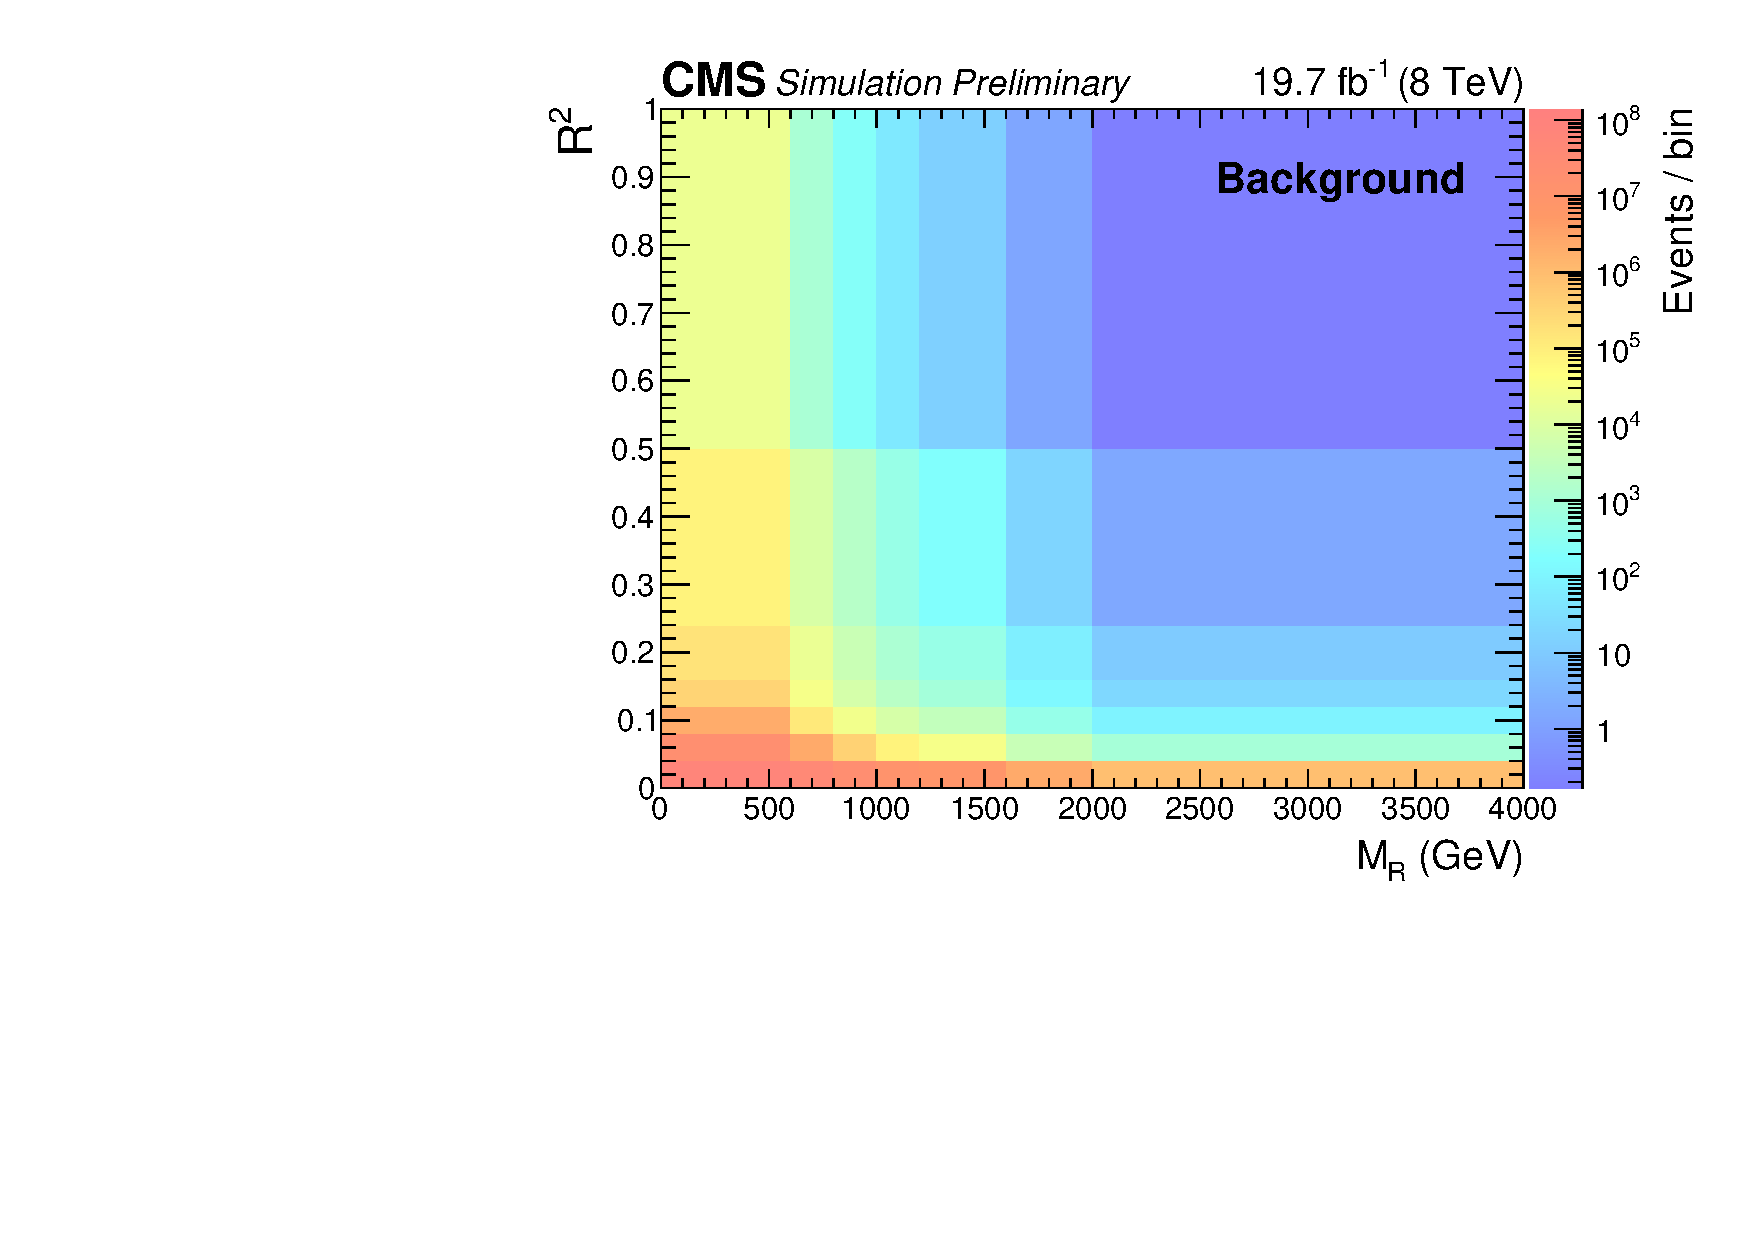
\includegraphics[width=0.49\textwidth]{figures/razor_variables/MR_R2_jet1ptg200_bg} 
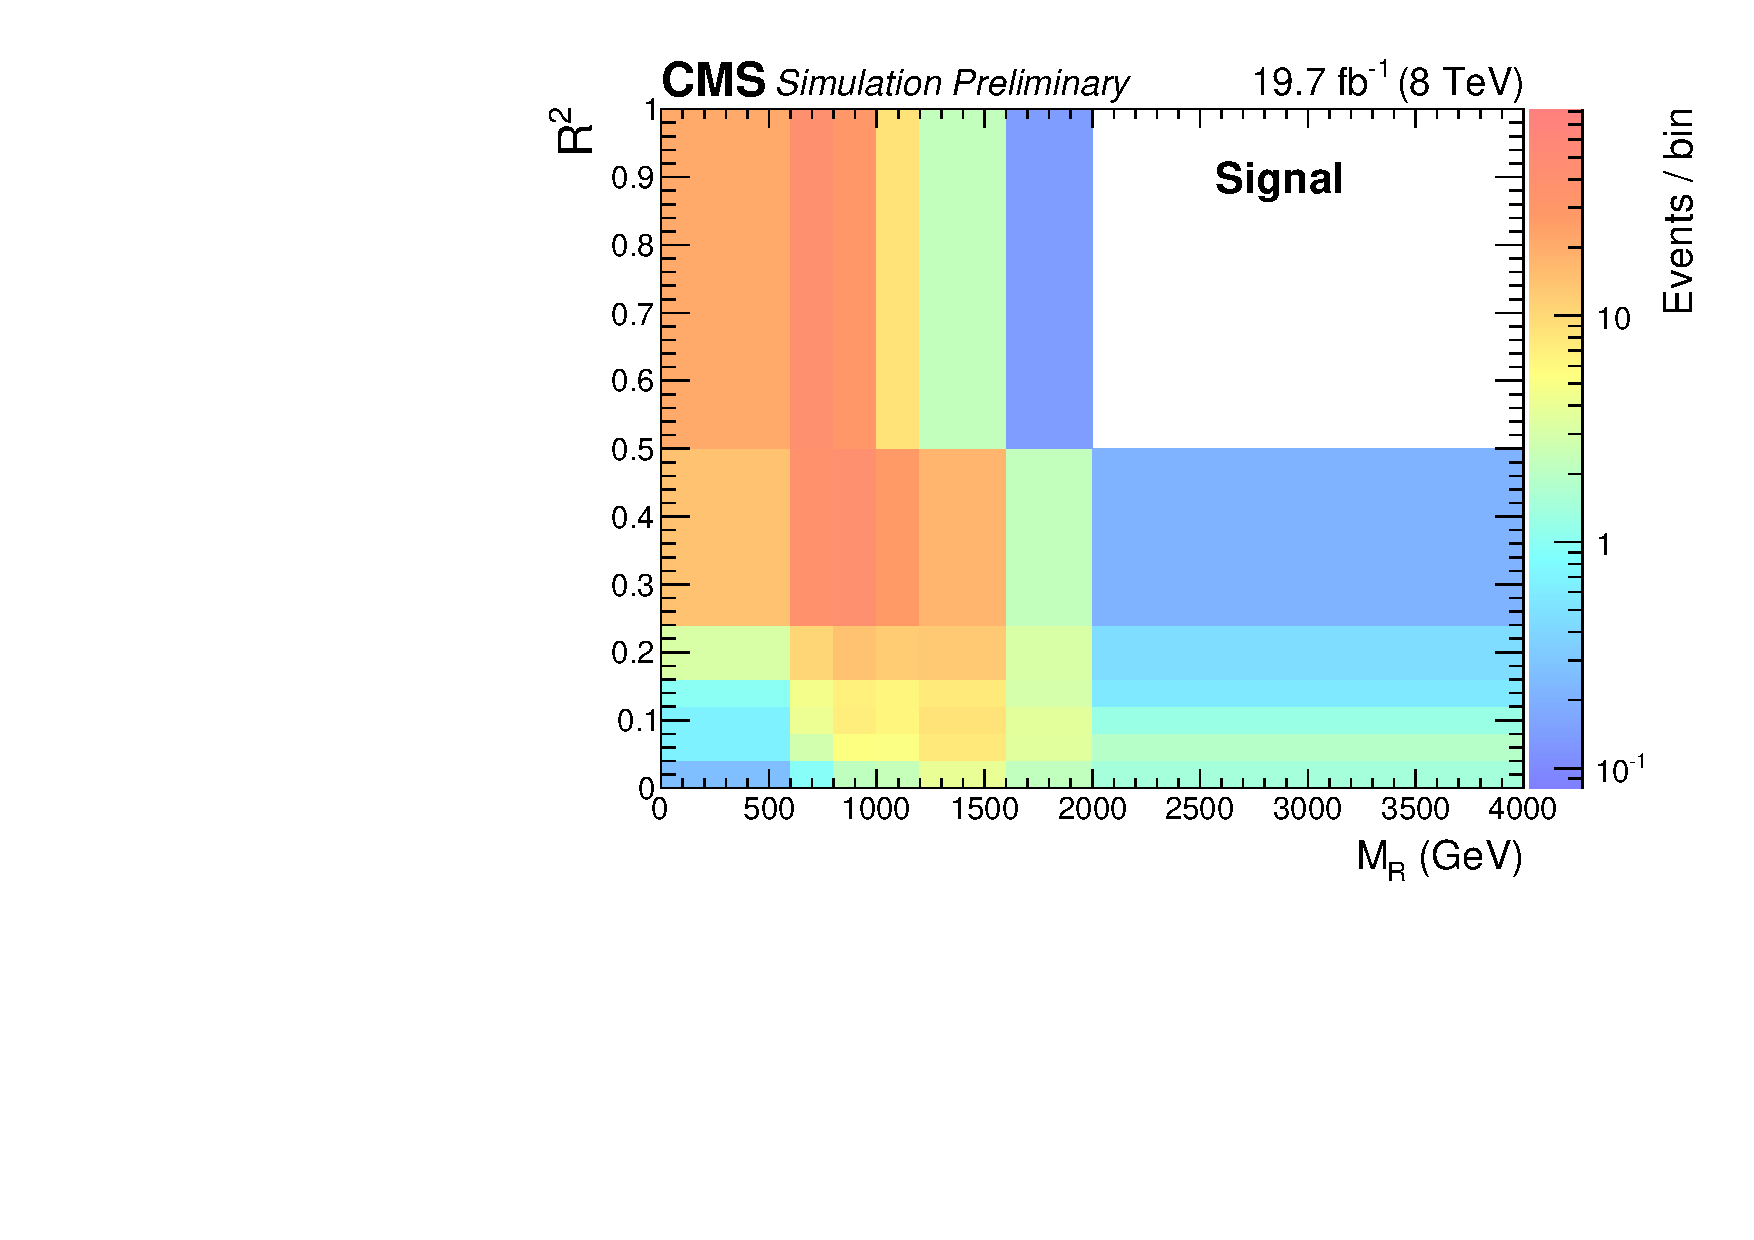
\includegraphics[width=0.49\textwidth]{figures/razor_variables/MR_R2_jet1ptg200_sig}
\caption{Distribution of the overall SM backgrounds and a T1ttcc signal with $m_{\tilde{g}} \,{=}\,
1\TeV$, $m_{\tilde{t}} \,{=}\, 325\GeV$ and $m_{\tilde{\chi}_1^0} \,{=}\, 300\GeV$, both obtained
from MC, on the (\mr,\rsq) space. A very loose selection is used:  a good primary vertex and at
least three jets, one of which should have $\pt > 200$ \GeV. 
\label{fig:razor_MR_Rsq_bg_signal}}

\end{figure}




\section[Boosted W boson tagging]{Boosted $\W$ boson tagging \label{sec:boost_wtag}}

%%%%%%%%%%%%%%%%%
% W tagging
%%%%%%%%%%%%%%%%%

One of the main highlights of the razor boost analysis is the tagging of boosted $\W$ bosons in
order to access a signal dominated phase space. 
$\W$ bosons either decay to two quarks, or to a lepton and a neutrino. The razor boost analysis is
an all-hadronic analysis, which means we do not explicitly consider the leptonic decays. 
$\W$ bosons with low to moderate transverse momentum will thus result in two jets, corresponding to
the two clusters of particles resulting from the hadronization of the two quarks. 
As the $\pt$ of the $\W$ boson increases, the separation between the two resulting jets decreases.
For high enough momentum, the two jets can no longer be fully resolved with the usual jet
definitions, and will be reconstructed as a single jet. This turnover in efficiency between the
resolved and merged case is illustrated in Fig.~\ref{fig:boost_wtag_ca8eff}.
Depending on the requirements on the jet multiplicity, losing a jet can result in a loss of signal
efficiency. We can, however, also use this effect to our advantage, namely to increase the
signal-to-background ratio by requiring the presence of one of these \textit{merged} jets. 
This, in turn, allows us to relax the jet multiplicity requirements. 

\begin{figure}
  \centering
  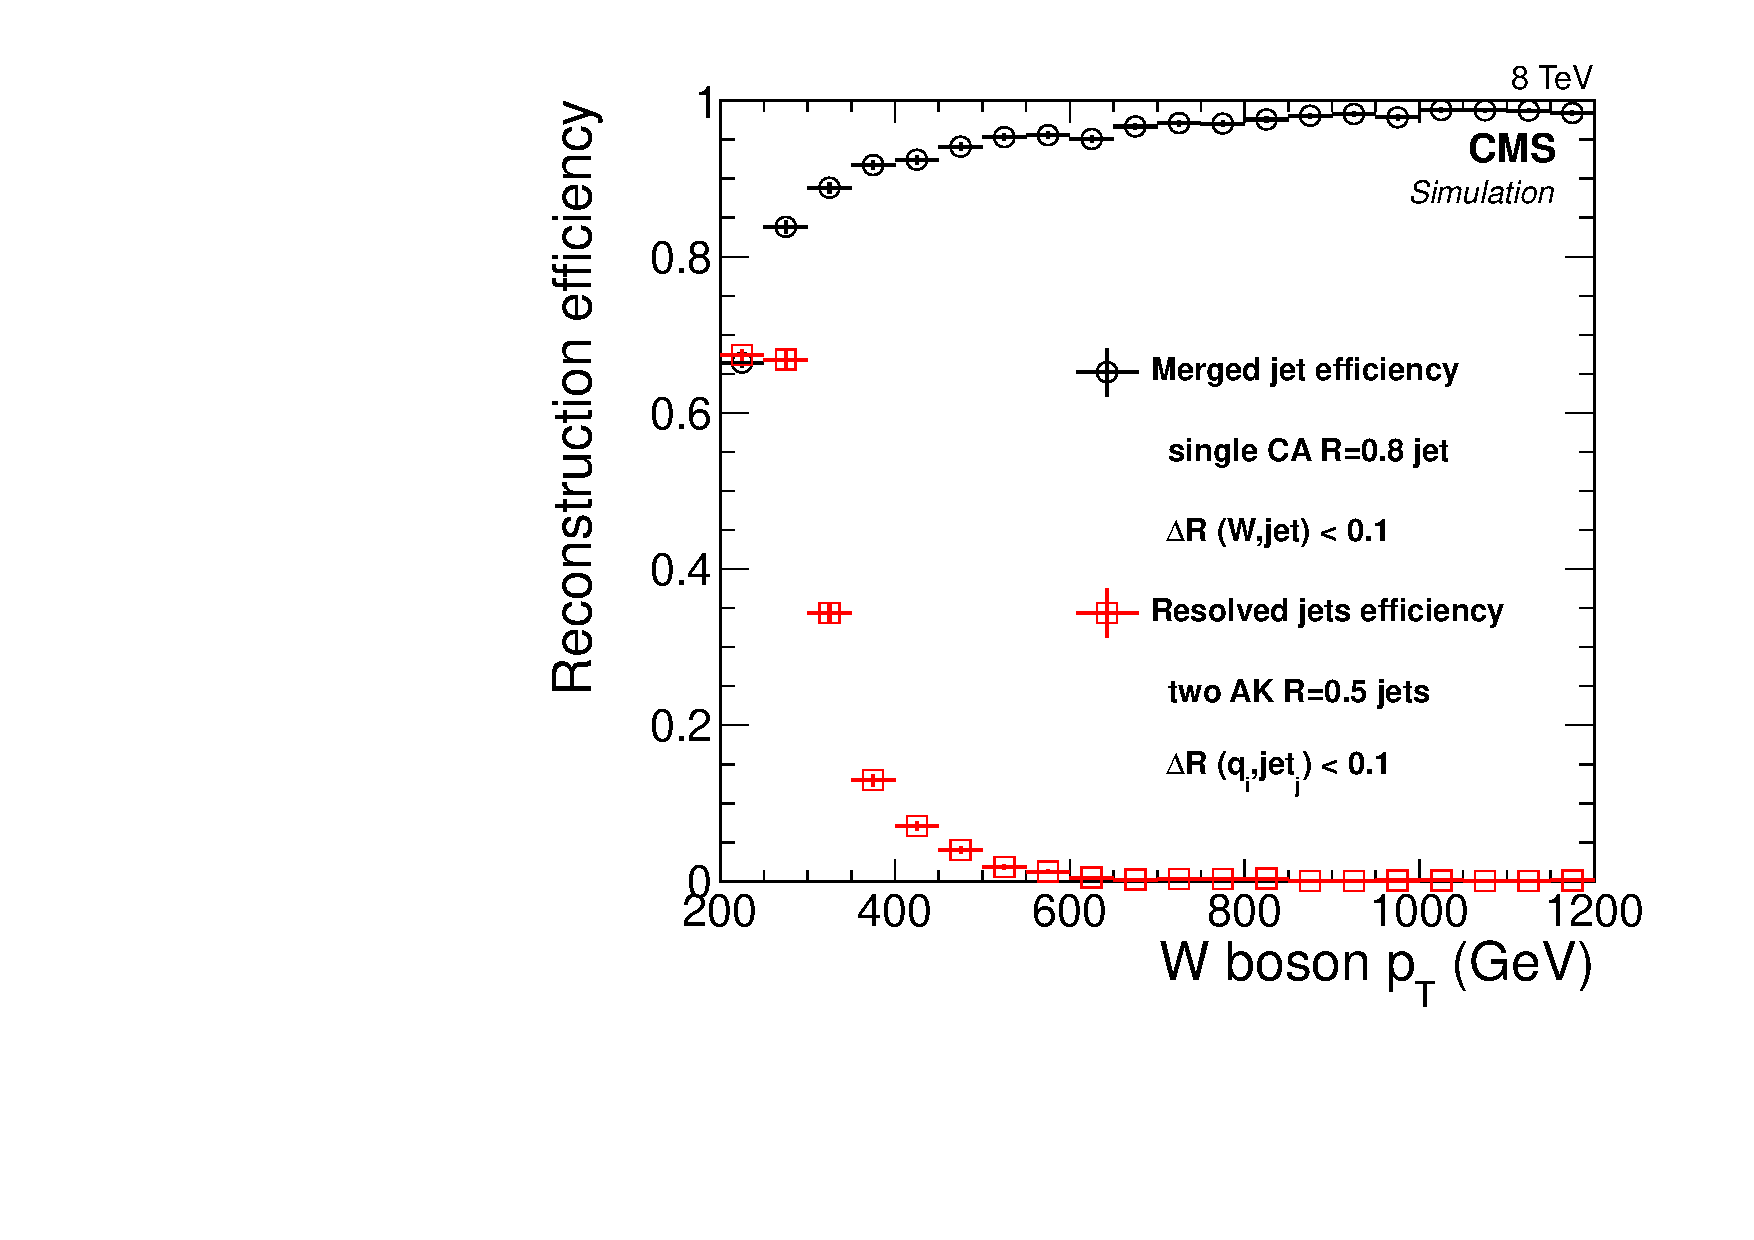
\includegraphics[width=0.8\textwidth]{figures/razor_wtag/ca8effVsPt}
  \caption{Efficiency to reconstruct a CA8 jet within $\Delta R<0.1$ of a generated $\W$ boson, and
the efficiency to reconstruct two AK5 jets within $\Delta R<0.1$ of the generated quarks from
longitudinally polarized $\W$ bosons, as a function of the $\pt$ of the $\W$
boson~\cite{Khachatryan:2014vla}. The loss in efficiency for the resolved case is clearly visible
for high $\pt$ $\W$ bosons. 
  \label{fig:boost_wtag_ca8eff}}
\end{figure}

The merged jet can be distinguished from other jets by its jet substructure, as illustrated in
Fig.~\ref{fig:boost_wtag_cartoon}. Jets originating from a $\W$ boson should have a two-prong
structure, whereas a quark/gluon-initiated jet is not expected to have this structure. 
In recent years, jet substructure techniques have seen very active developments, and many different
algorithms are on the market~\cite{Krohn:2009th,Gallicchio:2010sw,Butterworth:2008iy,Kaplan:2008ie}.
For the razor boost analysis we will use the CMS recommendation
in terms of which techniques to use~\cite{CMS-PAS-JME-13-006,Khachatryan:2014vla}. We will employ
\textit{jet pruning} and a set of variables called \textit{N-subjettiness}. On top of these jet
substructure techniques we will also use the jet mass variable to distinguish $\W$ boson-initiated
jets
from quark/gluon-initiated jets. 
The following subsections will go through the different parts of the
$\W$ tagging definition, providing a more detailed explanation for each.

\begin{figure}
  \centering
  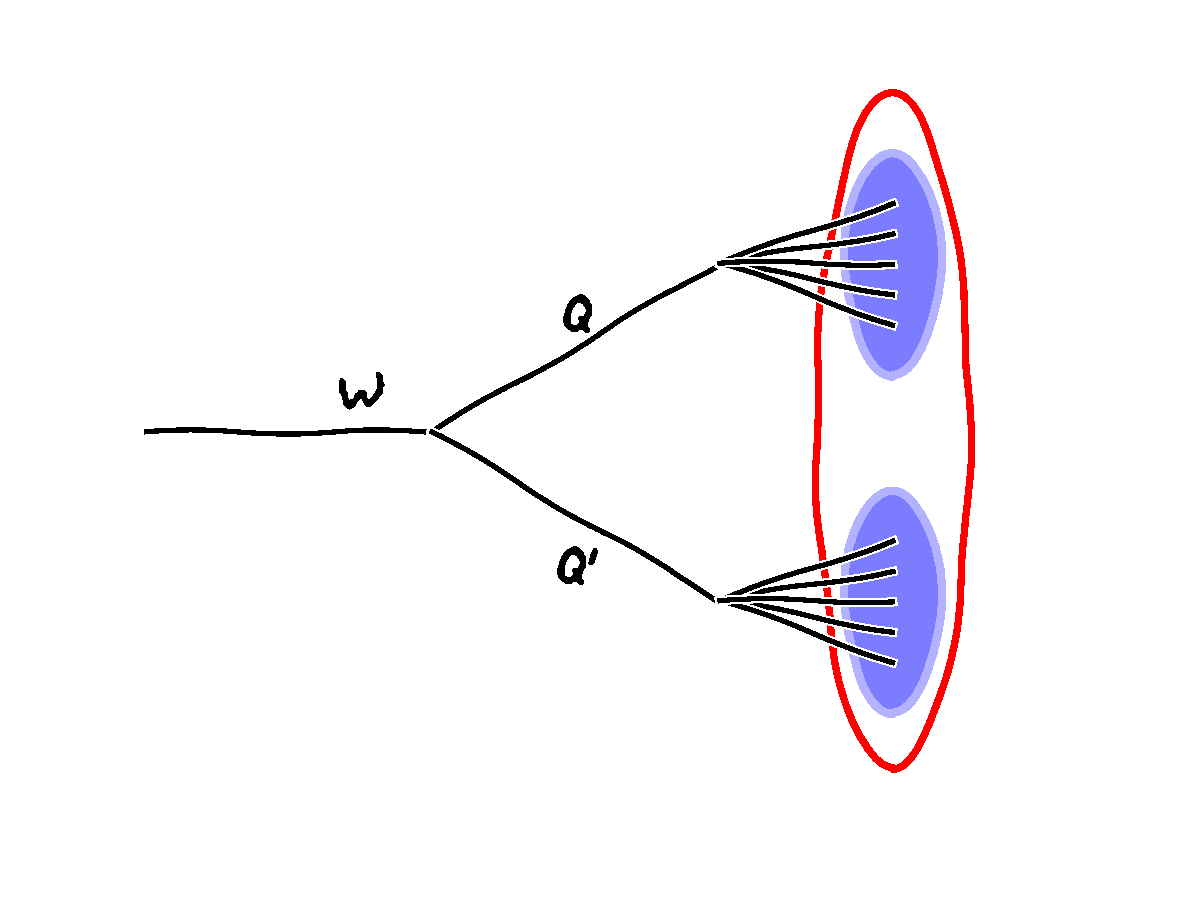
\includegraphics[width=0.48\textwidth]{figures/razor_wtag/W_subjets}
  ~
  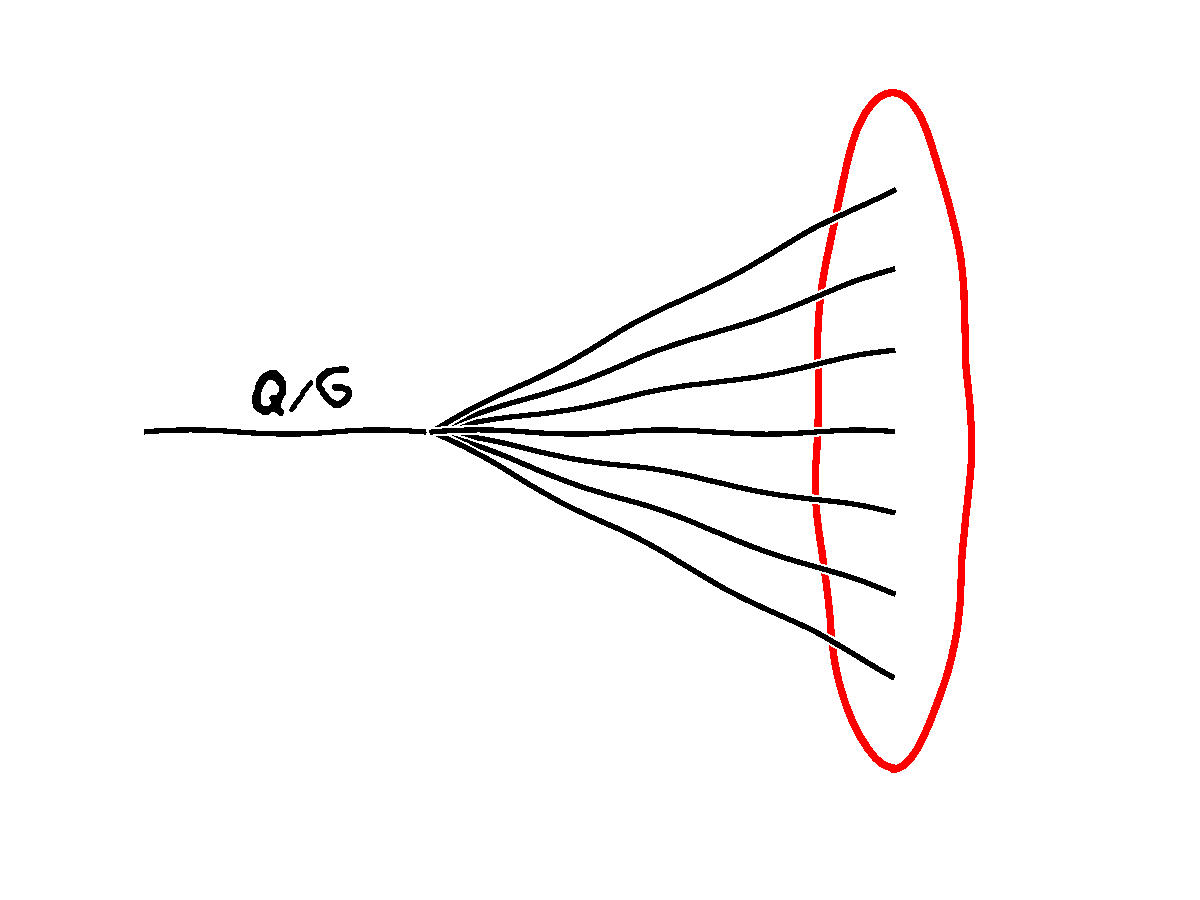
\includegraphics[width=0.48\textwidth]{figures/razor_wtag/qg_jets}
  \caption{The jet substructure of a $\W$-initiated jet differs from a quark/gluon-initiated jet.
  \label{fig:boost_wtag_cartoon}}
\end{figure}

%%%%%%%%%%%%%%%%%%%%%%%%%%%%%%%%%%%%%%%%%%%%%%%%%%%%%%%%%%%%%%%%%%%%%%%%%%%%%%%%%%%%%%%%%%%%%%%%%%%%

\subsection{Jet algorithm}

In order to identify boosted $\W$ bosons,  we will use a different jet clustering algorithm
than what is used for the standard jet definition (see Section~\ref{sec:object_jets}). 
Jets will be clustered with \textsc{FastJet 3.0.1.}~\cite{Cacciari:2011ma}, from the PF candidates,
using the Cambridge-Aachen (CA) algorithm~\cite{Dokshitzer:1997in} with a size parameter of 0.8.
Henceforth, we will call these jets \textit{CA8 jets}. 

%\begin{quote}
\begin{cajet} \theoremstyle{definition}
The Cambridge-Aachen jet algorithm is a sequential recombination algorithm that uses the
distance measure $d_{ij}$ between two constituents $i$ and $j$,
\begin{equation}
d_{ij} = \frac{\Delta R_{ij}^2}{R^2}, \label{eq:CA_distance}
\end{equation}
with $R$ the size parameter of the resulting jets, and
\begin{equation}
\Delta R_{ij}^2 = (y_i - y_j)^2 + (\phi_i - \phi_j)^2 ,
\label{eq:DeltaR_jet_algo}
\end{equation}
where $y, \phi$ are the rapidity (defined in Eq.~\ref{eq:rapidity}) and azimuthal angle. 
%The rapidity is given in terms of energy and longitudinal momentum as
%\begin{equation}
%  y = \frac{1}{2} \ln{\frac{ E + p_z }{ E - p_z }} .
%\end{equation}
The distance between constituent $i$ and the beam is given by $d_{iB} = 1$.
As is clear from the above, these distance measures only use angular information, unlike for the
$k_\mathrm{T}$ and anti-$k_\mathrm{T}$ algorithms, which use a $\pt$-weighted distance. 

The jet algorithm starts by computing the minimum distance $d_{ij}$, across all $i,j$. If $\min
d_{ij} < d_{iB}$, then we combine constituents $i$ and $j$ into a new constituent whose
four-momentum is the sum of the four-momenta of $i$ and $j$, and repeat the process. Otherwise, we
call $i$ a jet and move it from the list of constituents to be clustered to the list of final jets.
The process is repeated with the remaining constituents, until none remain.
\end{cajet}


Jet energy corrections for these CA8 jets are derived from the standard anti-$k_\textrm{T}$ jets
with size parameter $R=0.7$. Simulations show that the corrections are valid for CA8 jets and
have an additional uncertainty no greater than 2\%~\cite{CMS-PAS-JME-13-007,CMS-AN2012-393}.  
% seems like no better reference is available for this...

%%%%%%%%%%%%%%%%%%%%%%%%%%%%%%%%%%%%%%%%%%%%%%%%%%%%%%%%%%%%%%%%%%%%%%%%%%%%%%%%%%%%%%%%%%%%%%%%%%%%

\subsection{Jet pruning}

Jet pruning~\cite{Ellis:2009su,Ellis:2009me} is a particular kind of jet grooming. Jet grooming
techniques are designed to reduce the impact of contributions from the underlying event (UE), pileup
(PU), and low-\pt gluon radiation. These kinds of contributions to jets are typically soft and
diffuse, and increase the jet energy proportional to the jet area. Grooming techniques reduce the
jet area without affecting the core components. This means that the resulting jets are less
sensitive to these soft contributions, but still reflect the kinematics of the original, hard
process.


During jet pruning the constituents of the jet are reclustered with the CA algorithm, using the
same distance parameter as used for the original jets (here $R=0.8$), but with additional conditions
beyond those of the standard algorithm.
In particular, the softer and larger-angle of the two particles $i$ and $j$ to be merged is removed
when the following conditions are satisfied:
\begin{align}
  z_{ij} &= \frac{\min( \pt^i , \pt^j )}{\pt^i + \pt^j} < z_{\textrm{cut}}, \\
  \Delta R_{ij} &> D_{\textrm{cut}} \equiv \alpha \frac{m_J}{\pt} ,
\end{align}
where $m_J$ and $\pt$ are the original mass and transverse momentum of the reclustered jet,
$\Delta R_{ij}$ is defined as in Eq.~\ref{eq:DeltaR_jet_algo}, and
$z_\textrm{cut}$ and $\alpha$ are parameters of the algorithm, chosen to be 0.1 and 0.5,
respectively~\cite{Chatrchyan:2013vbb}. 

The resulting pruned jet is used as further input to our $\W$ boson tagger. For the $\W$ decay
products to be collimated, we need a large transverse momentum. We will therefore require that the
pruned jets have $\pt > 200\GeV$. 
Because of the reduction of the effect of UE and PU, the jet mass variable as computed from the
constituents of the jet after jet pruning has a much better behaviour than if it was computed from
the unpruned jets, as seen on Fig.~\ref{fig:wtag_jet_pruning}. Jet pruning shifts the jet mass of
QCD jets
to smaller values, while maintaining the jet mass for $\W$ jets close to the $\W$ boson mass.

We will make the requirement that the pruned jet mass is consistent with the $\W$ boson mass,
\begin{equation}
  70 < m_{\textrm{pruned jet}} < 100 \GeV .
\end{equation}
Here, we have deviated from the standard interval used in CMS, starting at 60\GeV, as we found that
for our
kinematical region and signal topology we achieve better signal to background discrimination when
increasing the lower cut value to 70\GeV. 
%This provides good boosted $\W$ jet to quark/gluon jet discrimination. 

\begin{figure}
  \centering
  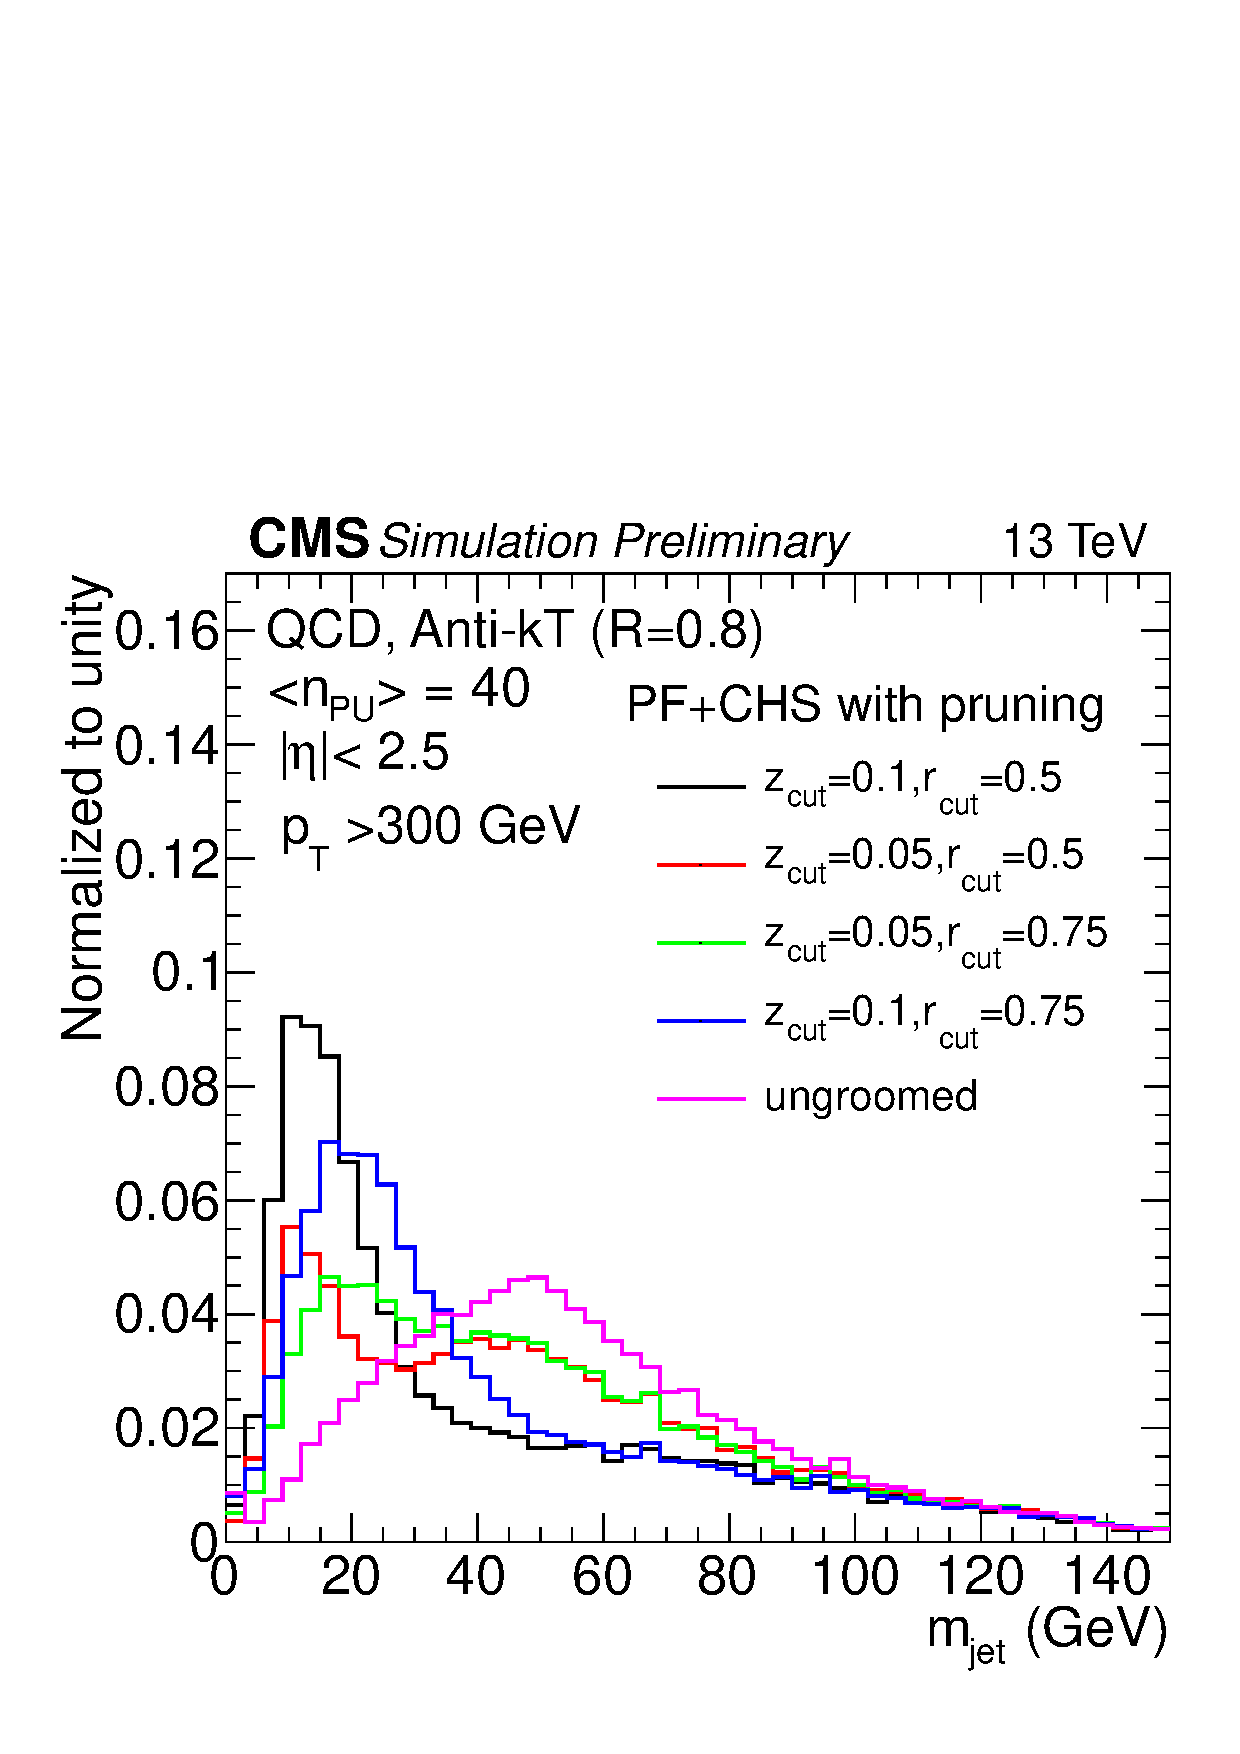
\includegraphics[width=0.6\textwidth]{figures/razor_wtag/1DPFCHS_PR_QCD}
  \caption{Jet mass distribution of QCD jets with $\pt(\textrm{gen}) > 300 \GeV$ for jet pruning
with different parameters, starting from PF jets with charged-hadron subtraction applied. The fully
ungroomed mass distribution is also shown for comparison. Here, the jets were clustered using the
anti-$k_\mathrm{T}$ algorithm, but the same picture holds for Cambridge-Aachen jets.
Figure taken from~Ref.\cite{CMS-PAS-JME-14-001}. 
  \label{fig:wtag_jet_pruning}}
\end{figure}

%%%%%%%%%%%%%%%%%%%%%%%%%%%%%%%%%%%%%%%%%%%%%%%%%%%%%%%%%%%%%%%%%%%%%%%%%%%%%%%%%%%%%%%%%%%%%%%%%%%%

\subsection{N-subjettiness}

Requiring the jet mass to be consistent with the $\W$ boson mass already results in a good
discrimination between $\W$ boson and quark/gluon-initiated jets. We can, however, still do better.
A boosted QCD jet with a mass around 80\GeV usually originates from a single hard parton and
acquires mass through large-angle soft splittings. The energy pattern for this process will differ
from the two-prong pattern that is found in boosted $\W$ jets.  
The set of N-subjettiness observables $\tau_N$~\cite{Thaler:2010tr} aims to exploit this difference
in expected energy flow to differentiate between $\W$ boson and quark/gluon-initiated jets by
counting the number of hard lobes of energy within a jet.

N-subjettiness is computed under the assumption that the jet has N subjets, and is the
$\pt$-weighted $\Delta R$ distance between each jet constituent and its nearest subjet axis:
\begin{equation}
\tau_N = \frac{1}{R_0 \sum_{k} p_{T, k}} \sum_k p_{T, k} \min (\Delta R_{1,k}, \Delta R_{2,k}, ...
\Delta R_{N,k}),
\end{equation}
where $R_0$ is the original jet distance parameter (0.8 in our case) and $k$ runs over all
constituent particles of the jet. 
The subjet axes are obtained by running the exclusive $k_T$
algorithm~\cite{Ellis:1993tq,Catani:1993hr} using \textsc{FastJet}. 
The exclusive $k_T$ algorithm differs from the inclusive version in two ways: if at a given
clustering step $d_{iB} < \min_j d_{ij}$, then constituent $i$ is discarded, rather than added to
the jet collection; and the clustering stops when the desired number of jets (N) is reached. 
The resulting axes can be further optimized to minimize the N-subjettiness value. In accordance to
the CMS recommendation, we use a “one-pass” optimization of the exclusive $k_T$
axes~\cite{nsubjettiness_fastjet}.

The variables $\tau_N$ quantify the consistency of the jet having N or fewer subjets. They have a
small value (close to 0) if the original jet is consistent with having N or fewer subjets, because
almost every jet constituent will be close in $\Delta R$ to its own true subjet. 
As we are interested in discriminating boosted $\W$ bosons, with two subjets, from quark/gluon
jets, which have a single subjet, we will use the variables $\tau_2$ and $\tau_1$, as obtained
from the unpruned CA8 jets.   
It has been shown that the ratio of the $\tau_N$ variables are better discriminators than the
separate variables~\cite{Thaler:2010tr}. We will thus require that the ratio $\tau_2 / \tau_1$ is
small. 
To ensure that the N-subjettiness ratio as computed from the unpruned
jet collection is assigned to the correct pruned jet, we find the highest \pt unpruned jet that is
within $\Delta R = 0.7$ of the considered pruned jet.
The $\tau_2 / \tau_1$ distribution for highly boosted and longitudinally polarized $\W$
bosons and for inclusive QCD jets is shown in Fig.~\ref{fig:boost_wtag_tau2tau1}. 

\begin{figure}[htb]
  \centering
  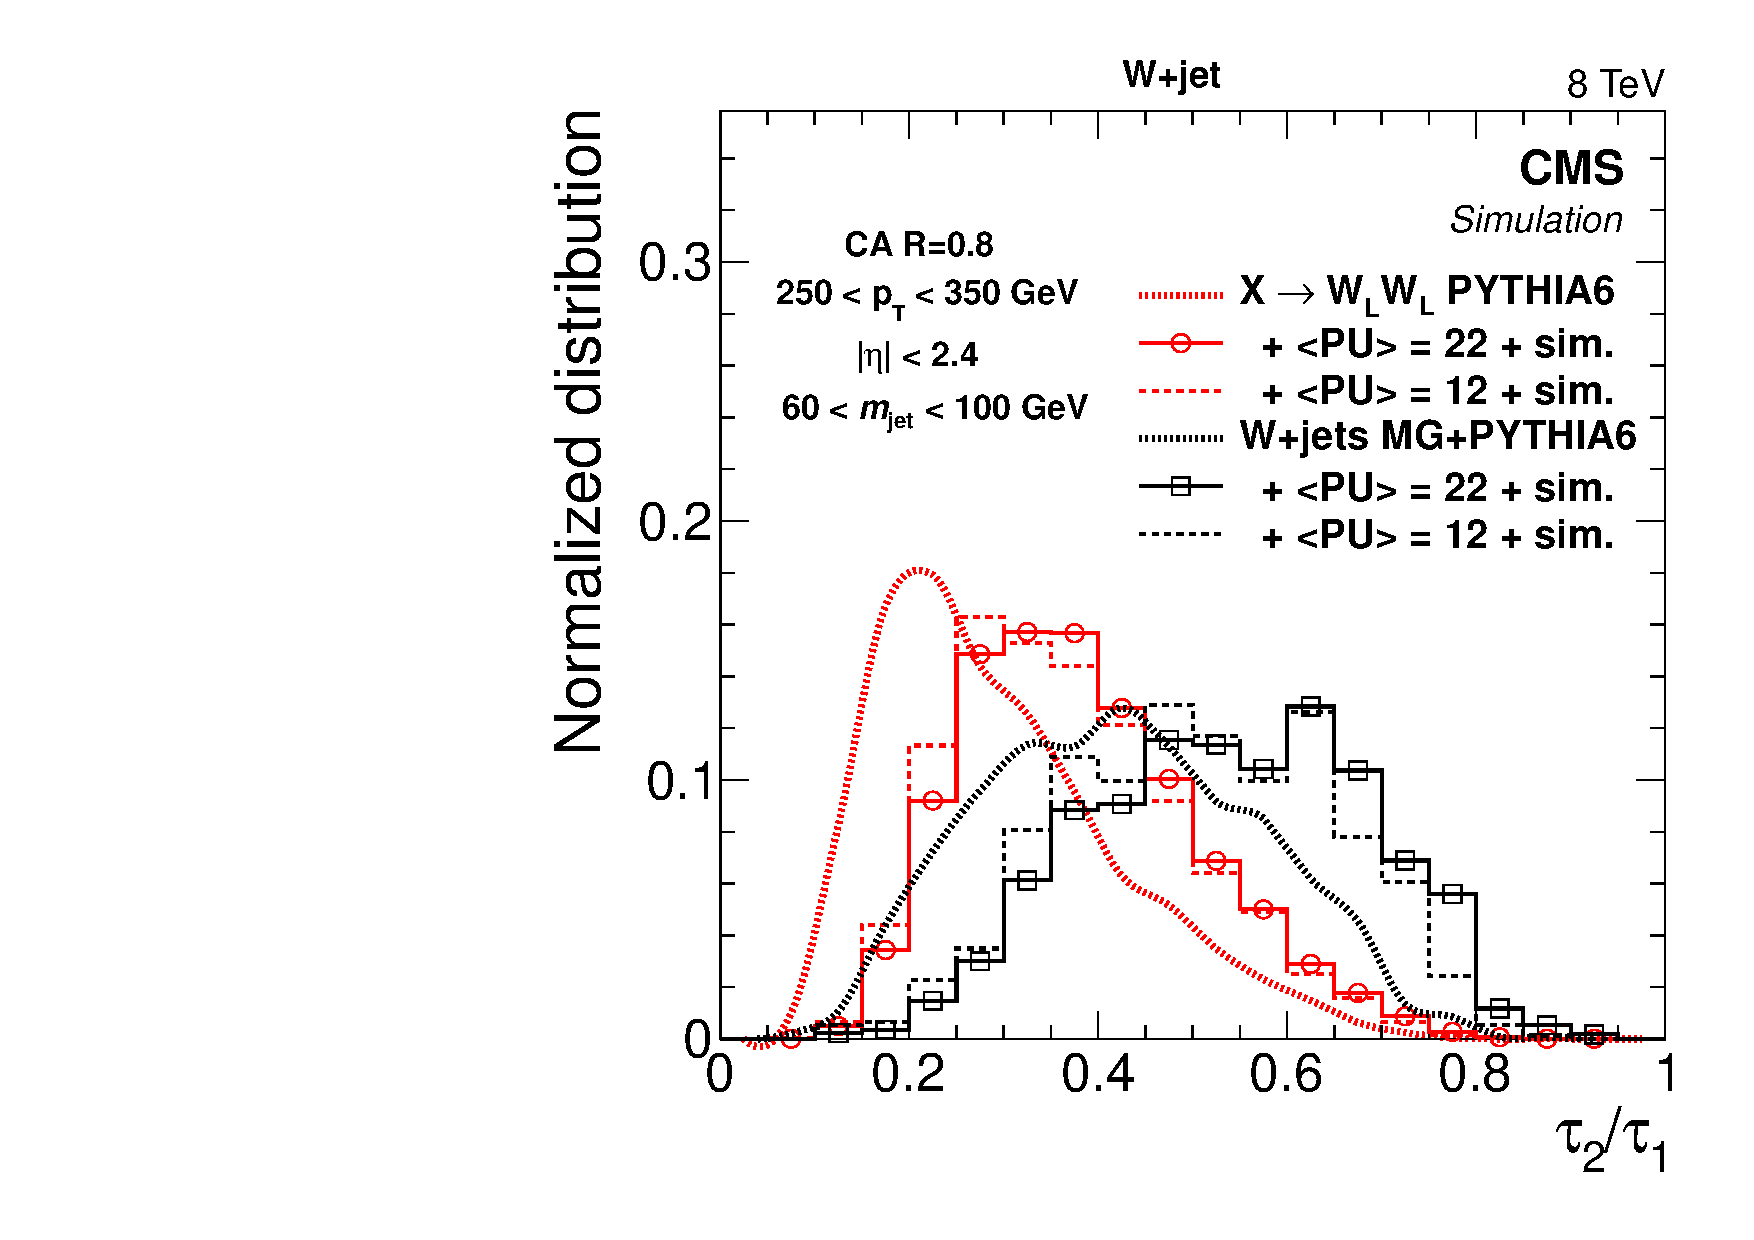
\includegraphics[width=0.8\textwidth]{figures/razor_wtag/tau2tau1_afterMass}
  \caption{Distributions of the N-subjettiness ratio $\tau_2 / \tau_1$ in simulated samples of
highly boosted and longitudinally polarized $\W$ bosons and inclusive QCD jets expected in the
$\W$+jet topology (\ie with leptonically decaying $\W$ bosons recoiling off a hard jet). 
The distribution is shown after a selection on the pruned jet mass of $60 < m_{\textrm{pruned jet}}
< 100 \GeV$. Note that this is slightly different from what is applied in the razor boost analysis.
Thick dashed lines represent the generator predictions without pileup interactions and without CMS
detector simulation. The histograms are the expected distributions after full CMS simulation with
pileup corresponding to an average number of 12 and 22 interactions~\cite{Khachatryan:2014vla}. 
  \label{fig:boost_wtag_tau2tau1}}
\end{figure}


%%%%%%%%%%%%%%%%%%%%%%%%%%%%%%%%%%%%%%%%%%%%%%%%%%%%%%%%%%%%%%%%%%%%%%%%%%%%%%%%%%%%%%%%%%%%%%%%%%%%

\subsection{\texorpdfstring{$\W$}{W} boson tagging definitions}

In the razor boost analysis we will employ a boosted $\W$ boson tagger, utilizing the techniques
outlined in the previous sections, to identify events that are consistent with the presence of a
high \pt, hadronically decaying $\W$ boson. 
A given pruned CA8 jet is $\W$ tagged if it has $\pt > 200\GeV$, $|\eta|<2.4$, $70 < m_\textrm{jet}
< 100\GeV$, and the corresponding unpruned jet satisfies $\tau_2 / \tau_1 < 0.5$.
This definition is the same as was used previously in a search for massive resonances in dijet
systems containing jets tagged as a W or Z boson~\cite{EXO-12-024,EXO-13-009}. 
The precise definition of this $\W$ boson tagger is summarized in Table~\ref{tab:Wtag_definition}.

As explained in Section~\ref{sec:boost_strategy}, we will use three control regions to select data
samples enriched in QCD multijet, $t\bar{t}$, and $\W(\rightarrow l \nu)+$jets, in order to help
model the SM backgrounds. QCD multijet and leptonically decaying $\W$+jets events are not expected
to have jets with a two-prong substructure. Therefore, our $\W$ boson tagging definition will not be
very efficient in selecting these processes. To remedy this, we slightly modify our $\W$ tagger. 
We define $\W$ boson \textit{anti-tagged} jets (aW) by taking the complement of the $\tau_2 /
\tau_1$ requirement, and define $\W$ boson \textit{mass-tagged} jets (mW) by dropping that
requirement all together. 
These definitions allow a more efficient selection of background processes, while remaining in a
similar kinematic regime. How these taggers will be used exactly will be explained in
Section~\ref{sec:boost_control_selection} when discussing the event selection. A summary of their
definitions can be found in Table~\ref{tab:Wtag_definition} as well. 

\begin{table}[htdp]
\caption{Boosted $\W$ tagging definitions. The input jet collection is either the pruned or unpruned
CA8 jet collection with charged-hadron subtraction applied. }
\vspace{1ex}
\centering
\begin{tabular}{l c c c}
\toprule
& $\W$ & aW & mW  \\
\midrule
\multirow{3}{*}{Pruned} & $\pt > 200$  & $\pt > 200$  & $\pt > 200$\\
& $|\eta| < 2.4$ & $|\eta| < 2.4$ & $|\eta| < 2.4$\\
& $70 < m_{\textrm{jet}}< 100$ & $70 < m_{\textrm{jet}}< 100$ & $70 < m_{\textrm{jet}}< 100$\\
\midrule
Unpruned & $\tau_2 / \tau_1 < 0.5$ & $\tau_2 / \tau_1 \geq 0.5$ & -\\
\bottomrule
\end{tabular}
\label{tab:Wtag_definition}
\end{table}

%%%%%%%%%%%%%%%%%%%%%%%%%%%%%%%%%%%%%%%%%%%%%%%%%%%%%%%%%%%%%%%%%%%%%%%%%%%

\subsection{\texorpdfstring{$\W$}{W} boson tagging scale factors \label{sec:wtag_scale_factor}}

It has been observed by previous CMS analyses that the $\W$ boson tagging efficiency is not the same
in data and in simulation. The distributions that are at the root of this disagreement are shown on
Fig.~\ref{fig:boost_wtag_data_sim}. 
To account for the discrepancies, we need to derive data/MC scale factors and associated
uncertainties corresponding to each of the $\W$ boson tagging, mass-tagging and anti-tagging
definitions listed in Table~\ref{tab:Wtag_definition}. These scale factors are not
process-independent. They will be different for processes that include hadronically decaying $\W$
bosons, such as $t\bar{t}$ or the signal, compared to processes which do not have $\W$ bosons in
their final state, such as QCD multijet production. For processes without real hadronically
decaying $\W$ bosons, any tagged jet is necessarily a misidentified, or \textit{fake}, $\W$ boson
tag. For those processes we will speak of the $\W$ boson tagging fake rate scale factors, where the
fake rate is defined as the probability to tag, with one of the used $\W$ tagging definitions, a jet
not coming from a hadronically decaying $\W$ boson. 
One last consideration concerns the signal simulation. As the signal is simulated with FastSim, we
need an additional scale factor to correct for differences in the modelling of the $\W$ tagger
between FastSim and FullSim. 
In the following subsections every scale factor will be listed in more detail, including how it was
derived and how it will be used in the analysis. 

\begin{figure}[htpb]
  \centering
  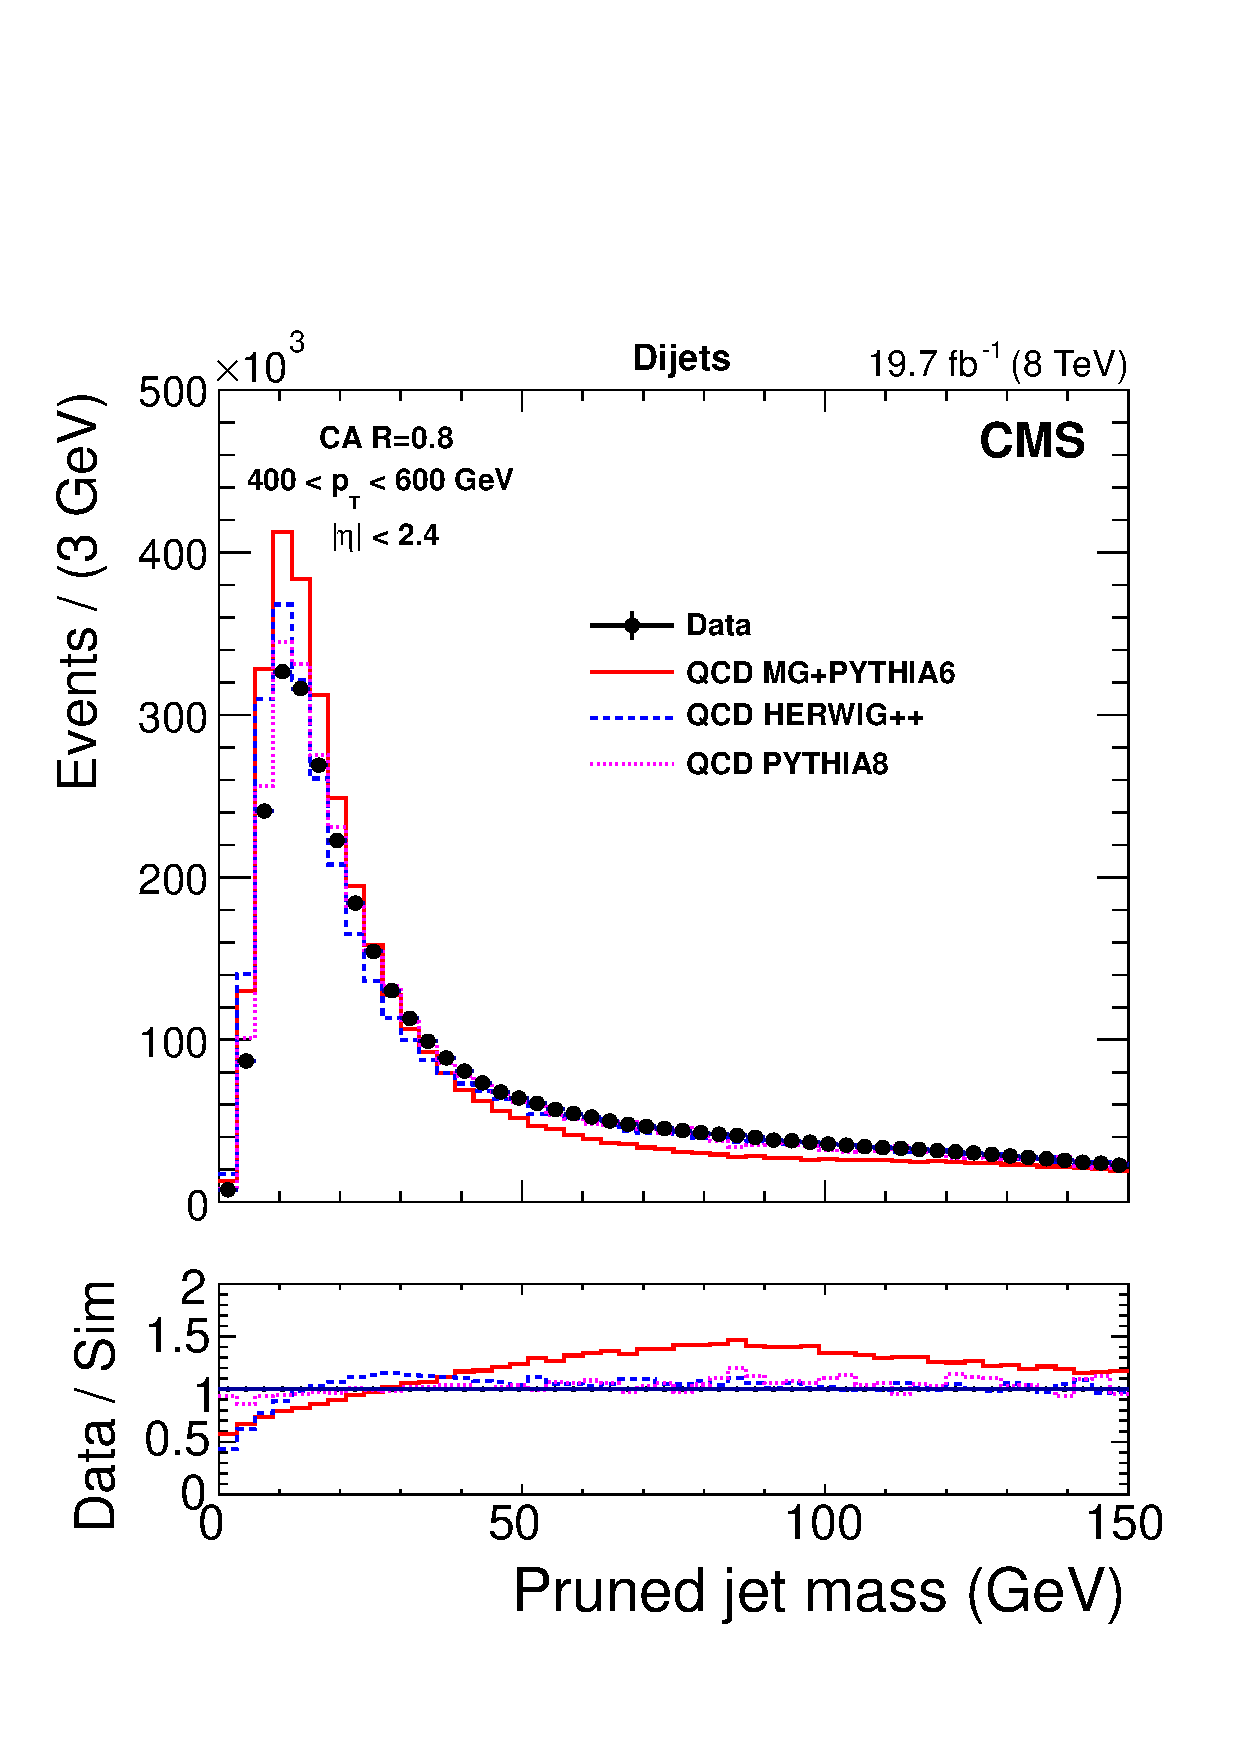
\includegraphics[width=0.48\textwidth]{figures/razor_wtag/substructure_pas_mass_2}
  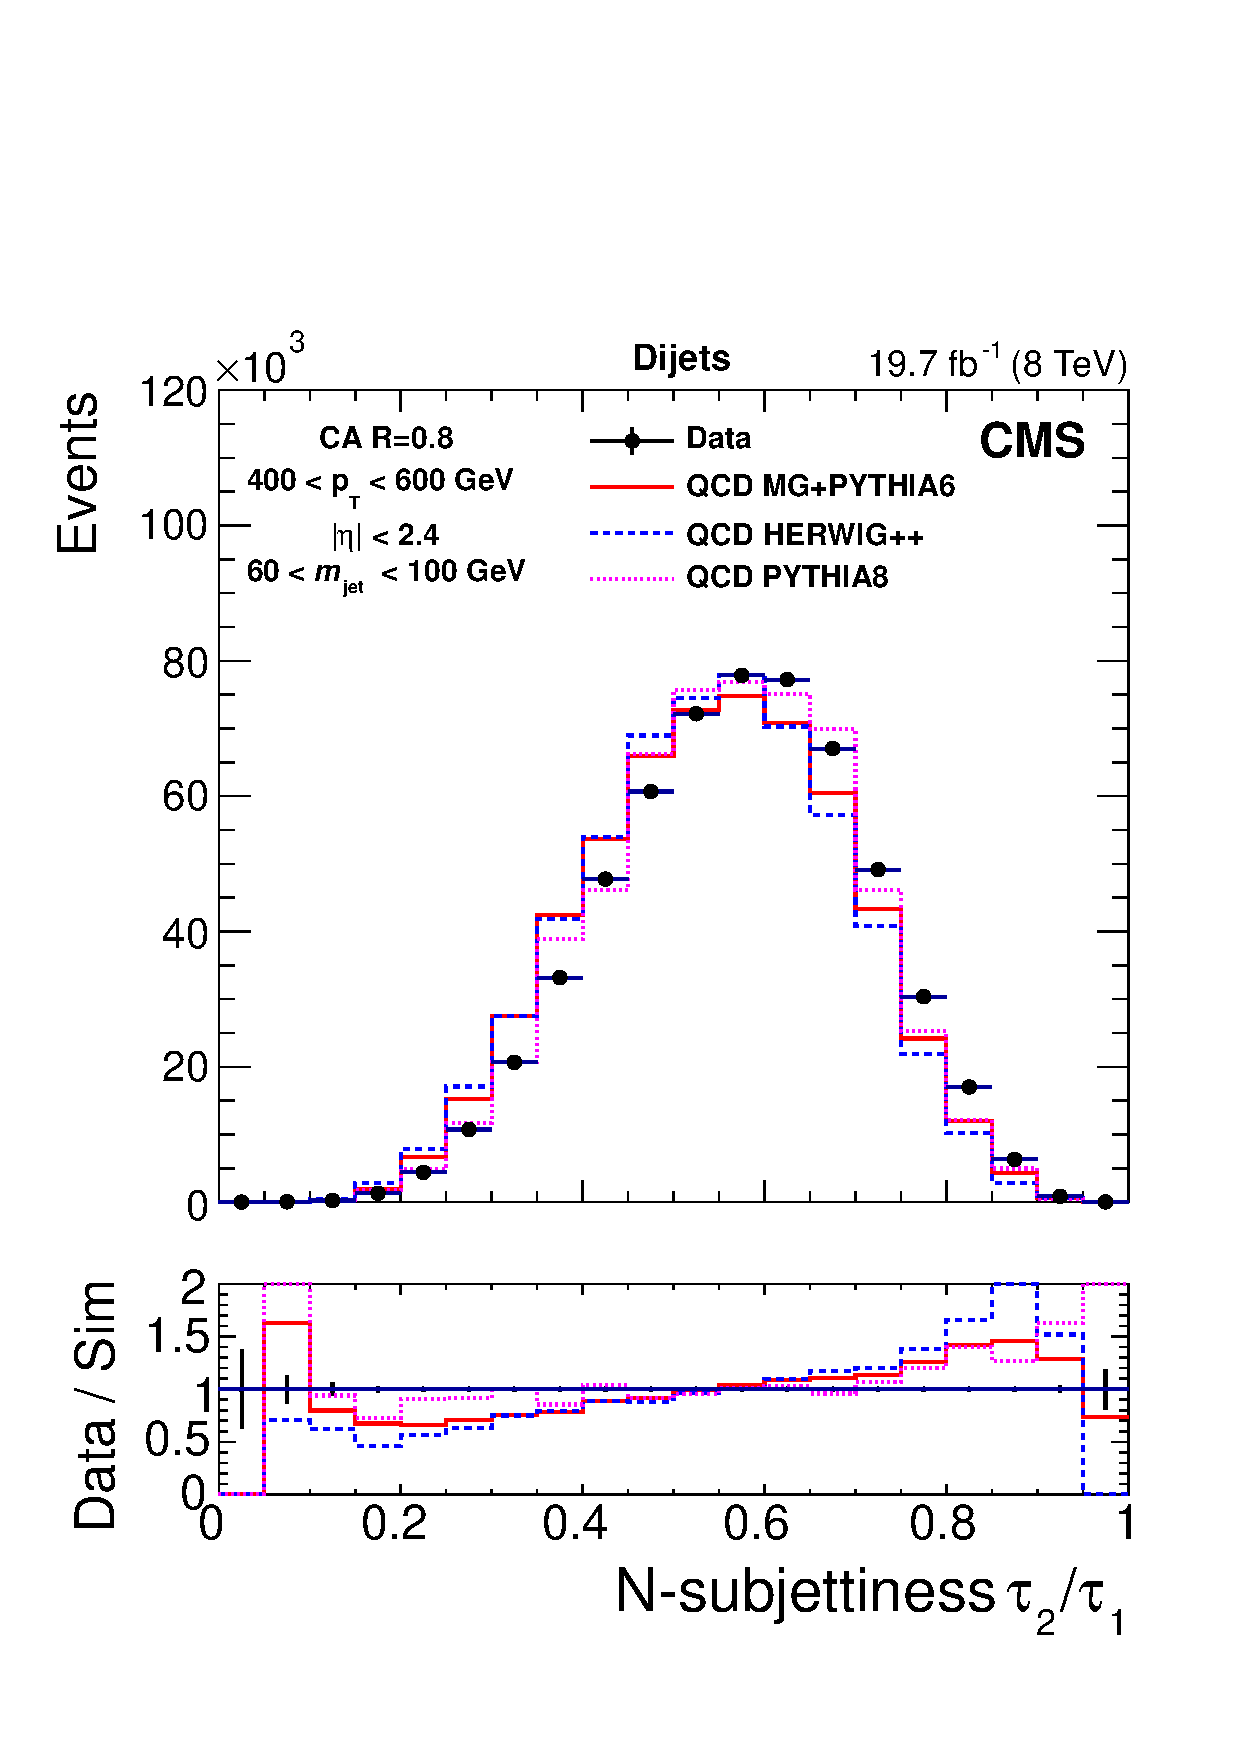
\includegraphics[width=0.48\textwidth]{figures/razor_wtag/substructure_pas_tau21_aftermass_2}
  \caption{Pruned jet mass (left) and N-subjettiness ratio $\tau_2/\tau_1$ (right) distributions 
  in data and simulation for dijet events. MG denotes the \MADGRAPH generator, and is the option
used for the razor boost analysis. The relative deviations between
data and simulation are plotted at the bottom of each figure~\cite{Khachatryan:2014vla}. 
  \label{fig:boost_wtag_data_sim}}  
\end{figure}

%% ---------------------------------------------------------------------------------------------

\subsubsection{\texorpdfstring{$\W$}{W} boson tag efficiency scale factor \label{sec:wtag_eff_sf}}

The $\W$ boson tag efficiency scale factor will be used to correct processes with real
hadronically decaying $\W$ bosons. For the backgrounds this is mainly for the $t\bar{t}$ process,
but also single top and $t\bar{t}$ in association with a $\W$ or $\cPZ$ boson are considered. This
scale factor is of course also used for the signal processes. 

The $\W$ boson tag efficiency scale factor is only applied to the simulation in the $S$ and $T$
region, see Sections~\ref{sec:boost_signal_selection} and \ref{sec:boost_T_region}, as those are the
regions that utilize the $\W$ tagging definition in their selection criteria. It is also only
applied to events for which the $\W$ boson tagged jet is matched (within a cone of $\Delta R = 0.8$)
to a generator level hadronically decaying $\W$ boson. In case no match was found, we apply the $\W$
boson tag fake rate scale factor. 

As we use the same $\W$ boson tagging definition as was used in a search for massive resonances in
dijet systems containing $\W$ tagged jets~\cite{EXO-12-024}, we can directly apply the scale
factor that was derived for that study. The
method used to obtain the scale factor is outlined in Ref.~\cite{CMS-PAS-JME-13-006}. 
The $\W$ boson tag efficiency scale factor $SF_{\textrm{Wtag}}$ is given by
\begin{equation}
SF_{\textrm{Wtag}} = 0.86 \pm 0.07 .
\end{equation}


%% ---------------------------------------------------------------------------------------------

\subsubsection{\texorpdfstring{$\W$}{W} boson tag efficiency FullSim/FastSim scale factor
\label{sec:wtag_eff_fastfull_sf}}

For our signal samples, which are produced with FastSim, we have derived an additional $\W$ tag
efficiency FullSim/FastSim scale factor, $SF_{\textrm{Full/Fast}}$, which depends on the \pt
of the CA8 jet. This scale factor corrects for the different modelling of jets, jet
substructure, etcetera, in FastSim with respect to FullSim. The product of $SF_{\textrm{Wtag}}$ and
$SF_{\textrm{Full/Fast}}$ will be applied to the signal simulation. 

To compute the $\W$ boson tag efficiency FullSim/FastSim scale factor we use a sample of $t\bar{t}$
events simulated with both FullSim and FastSim. 
A FastSim versus FullSim comparison of the distributions of the pruned jet mass, the N-subjettiness
variables $\tau_1$, $\tau_2$ and their ratio $\tau_2/\tau_1$, both before and after requiring the
jets to satisfy the pruned jet mass window, is shown in
Figs.~\ref{fig:FastFull_jmass}--\ref{fig:FastFull_tau21}. It is clear that the agreement is not
perfect. The $\tau_2/\tau_1$ distribution for FastSim is shifted with respect to FullSim. This
disagreement will then of course be translated into the efficiencies, and thus the need for a scale
factor arises. 

\begin{figure}[htpb]
\centering
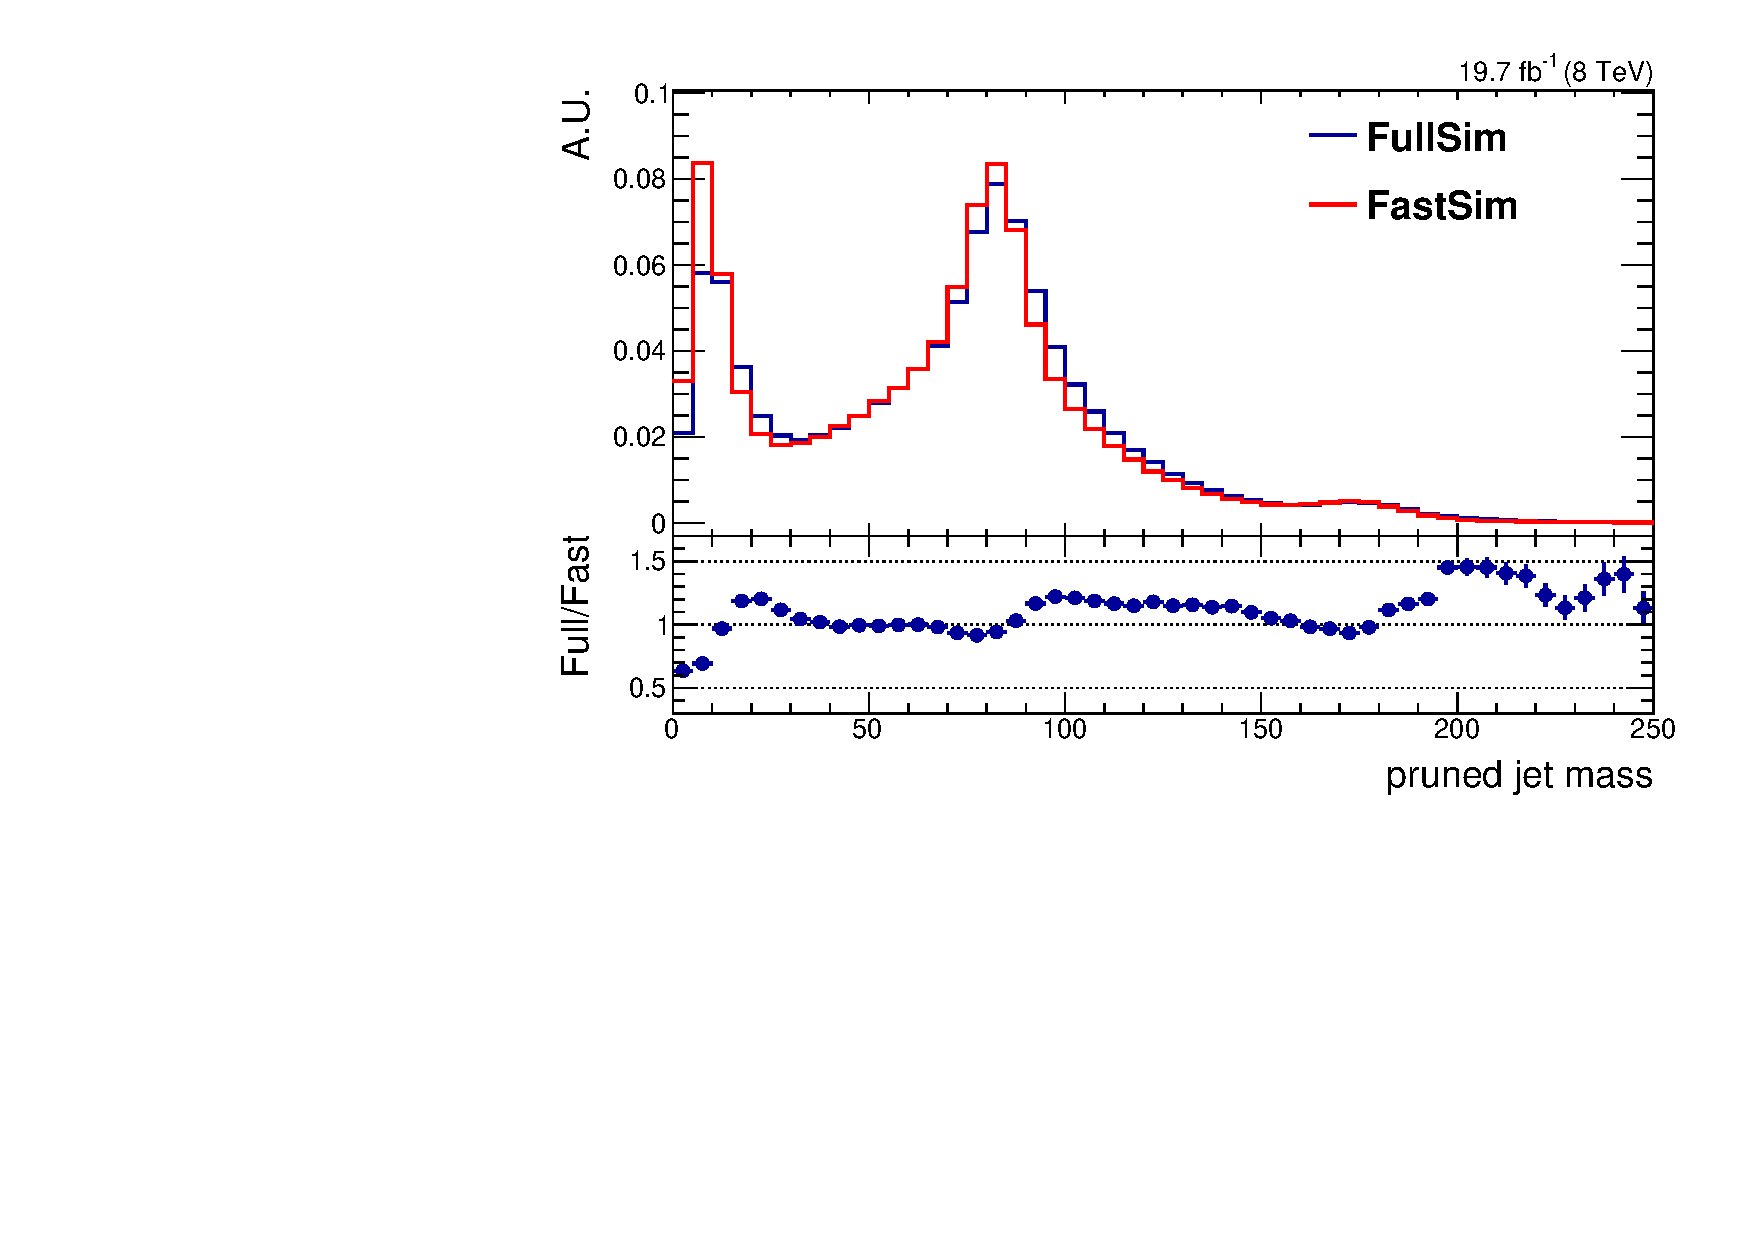
\includegraphics[width=0.7\textwidth]{figures/razor_wtag/FastFull_comparison_TTJets_jmass}
\caption{Pruned jet mass distribution for FastSim and FullSim $t\bar{t}$. 
\label{fig:FastFull_jmass}}
\end{figure}

\begin{figure}[p]
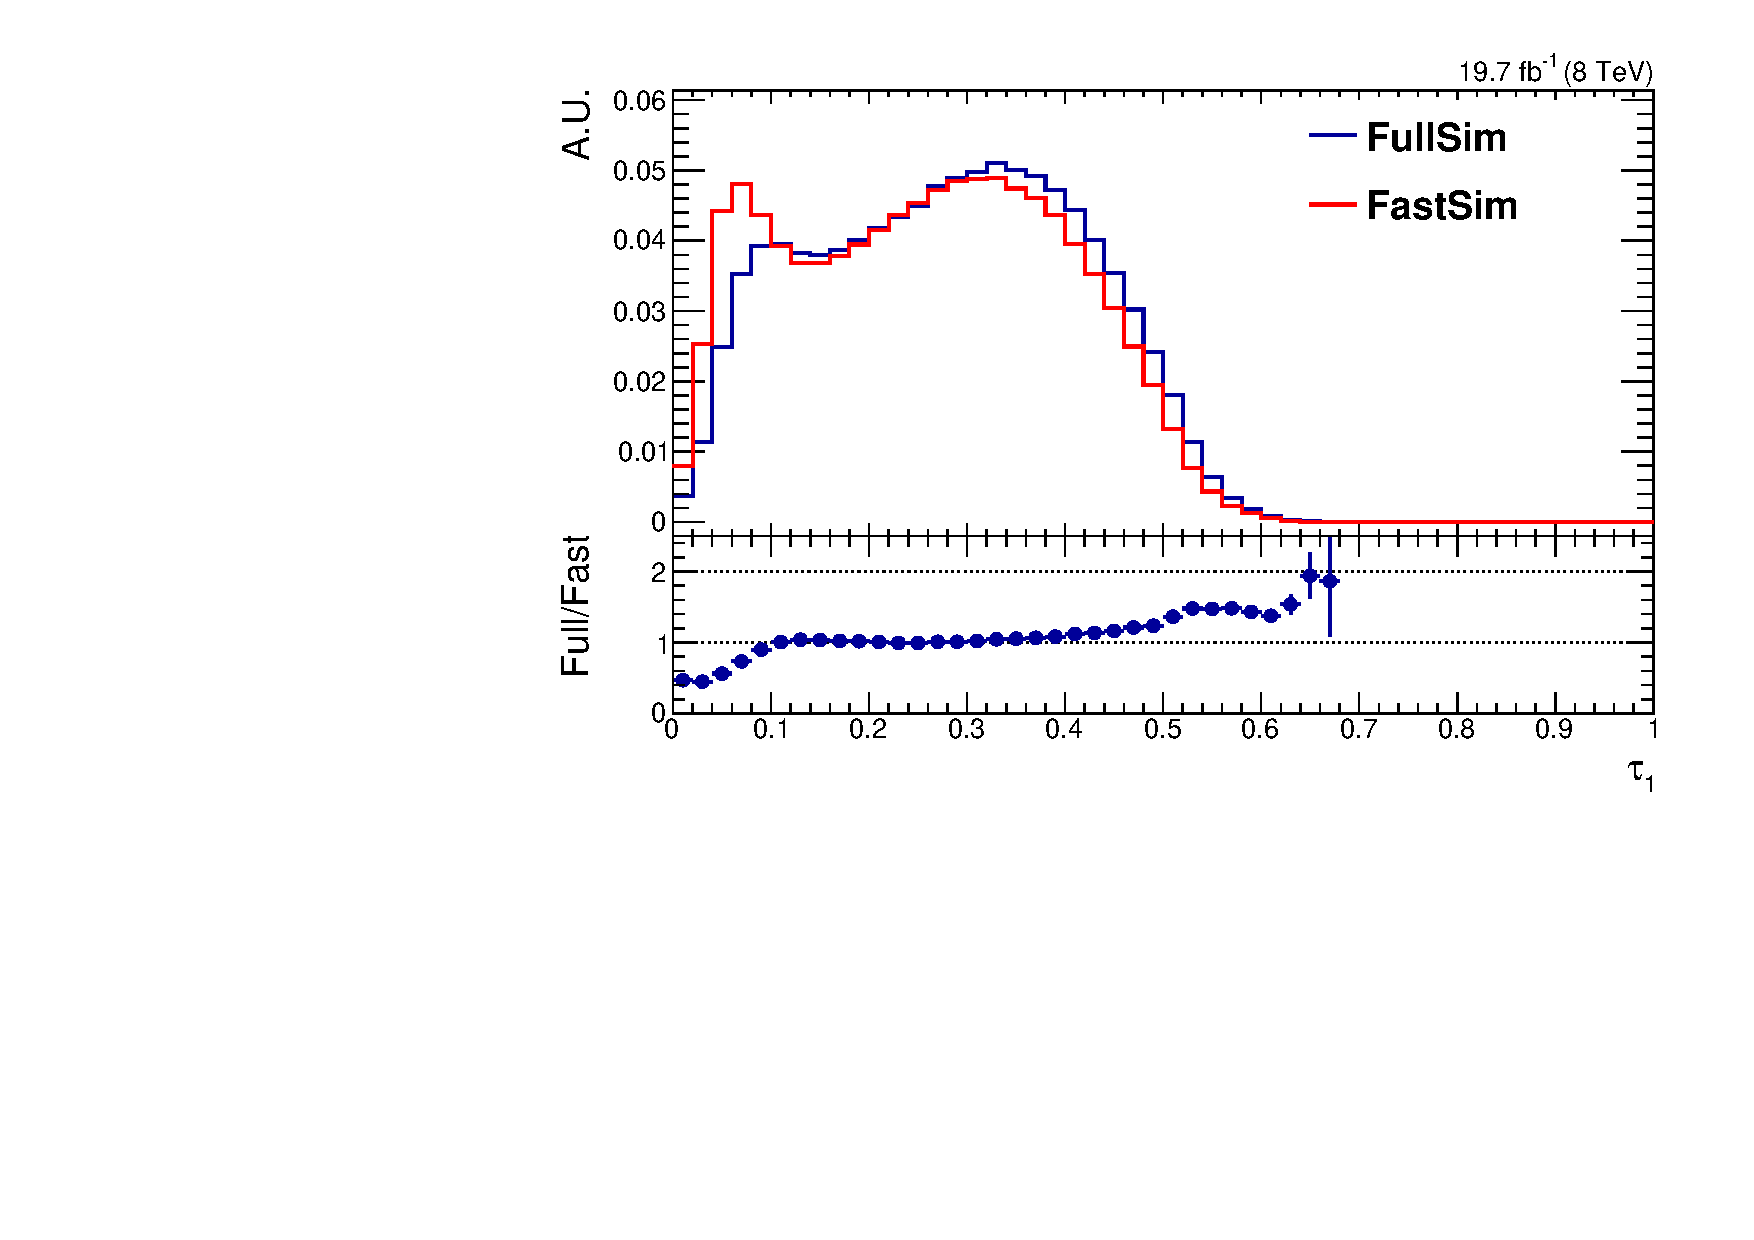
\includegraphics[width=0.49\textwidth]{figures/razor_wtag/FastFull_comparison_TTJets_tau1}
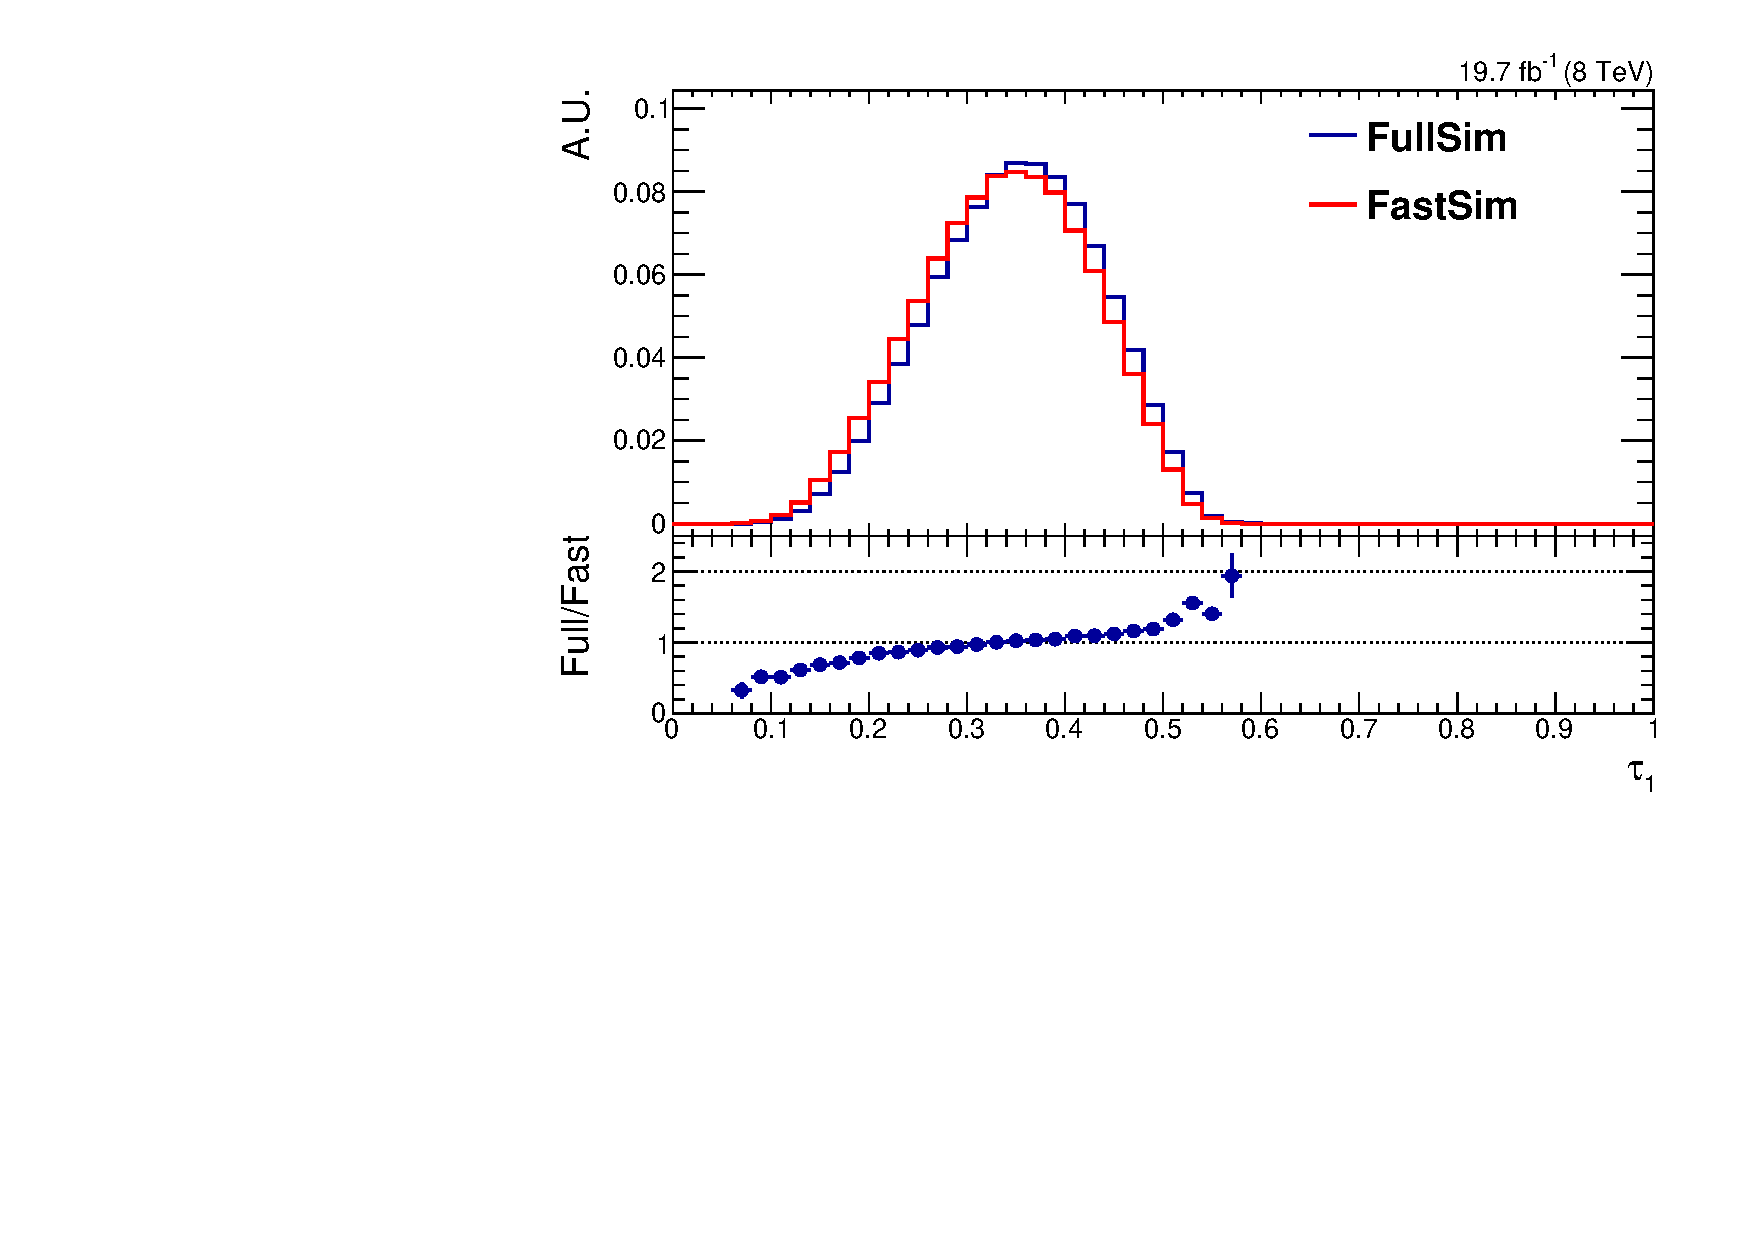
\includegraphics[width=0.49\textwidth]{figures/razor_wtag/FastFull_comparison_TTJets_tau1_masscut}
\caption{Distribution of $\tau_1$ before (left) and after (right) requiring the pruned CA8 jet to
lie within the $\W$ mass window, $70 < m_{\textrm{jet}} < 100$\GeV, for FastSim and
FullSim $t\bar{t}$.
\label{fig:FastFull_tau1}}
\end{figure}

\begin{figure}[p]
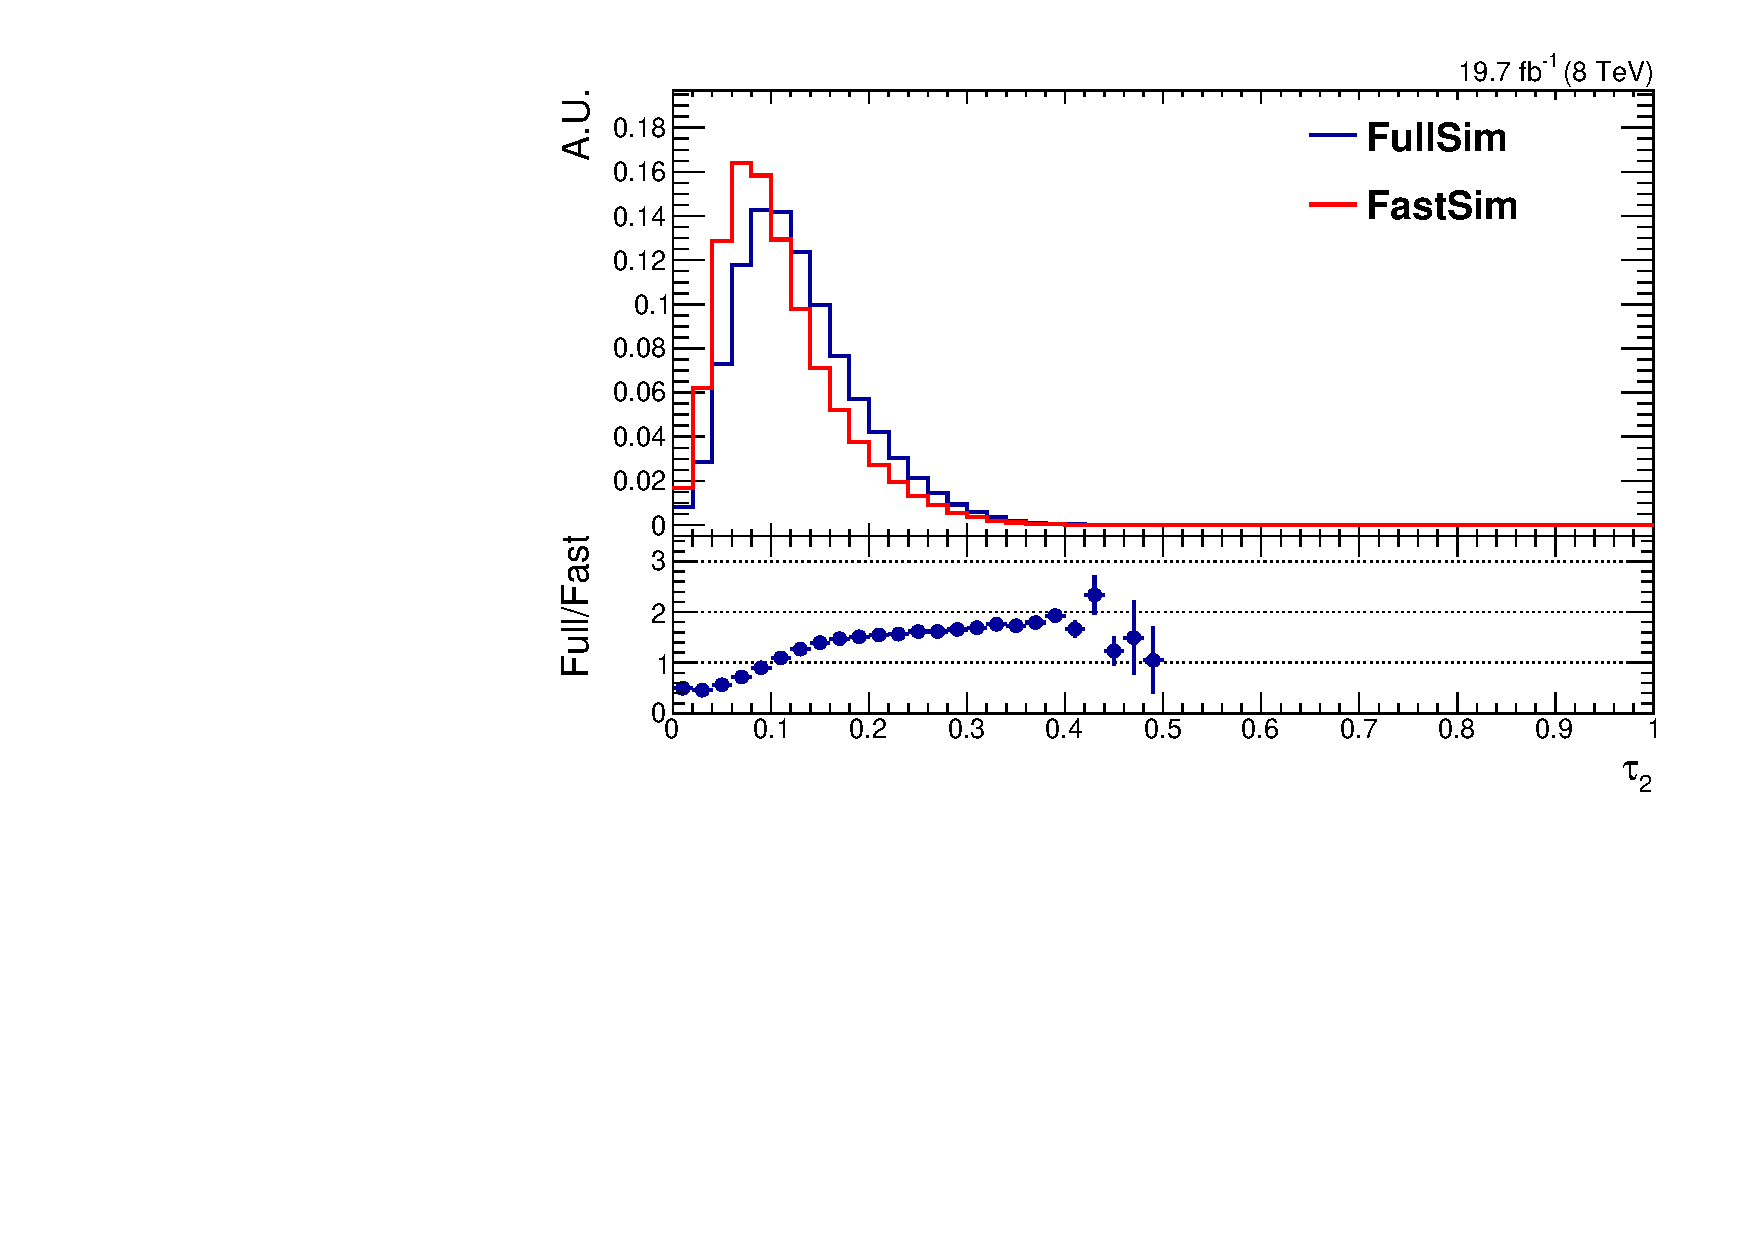
\includegraphics[width=0.49\textwidth]{figures/razor_wtag/FastFull_comparison_TTJets_tau2}
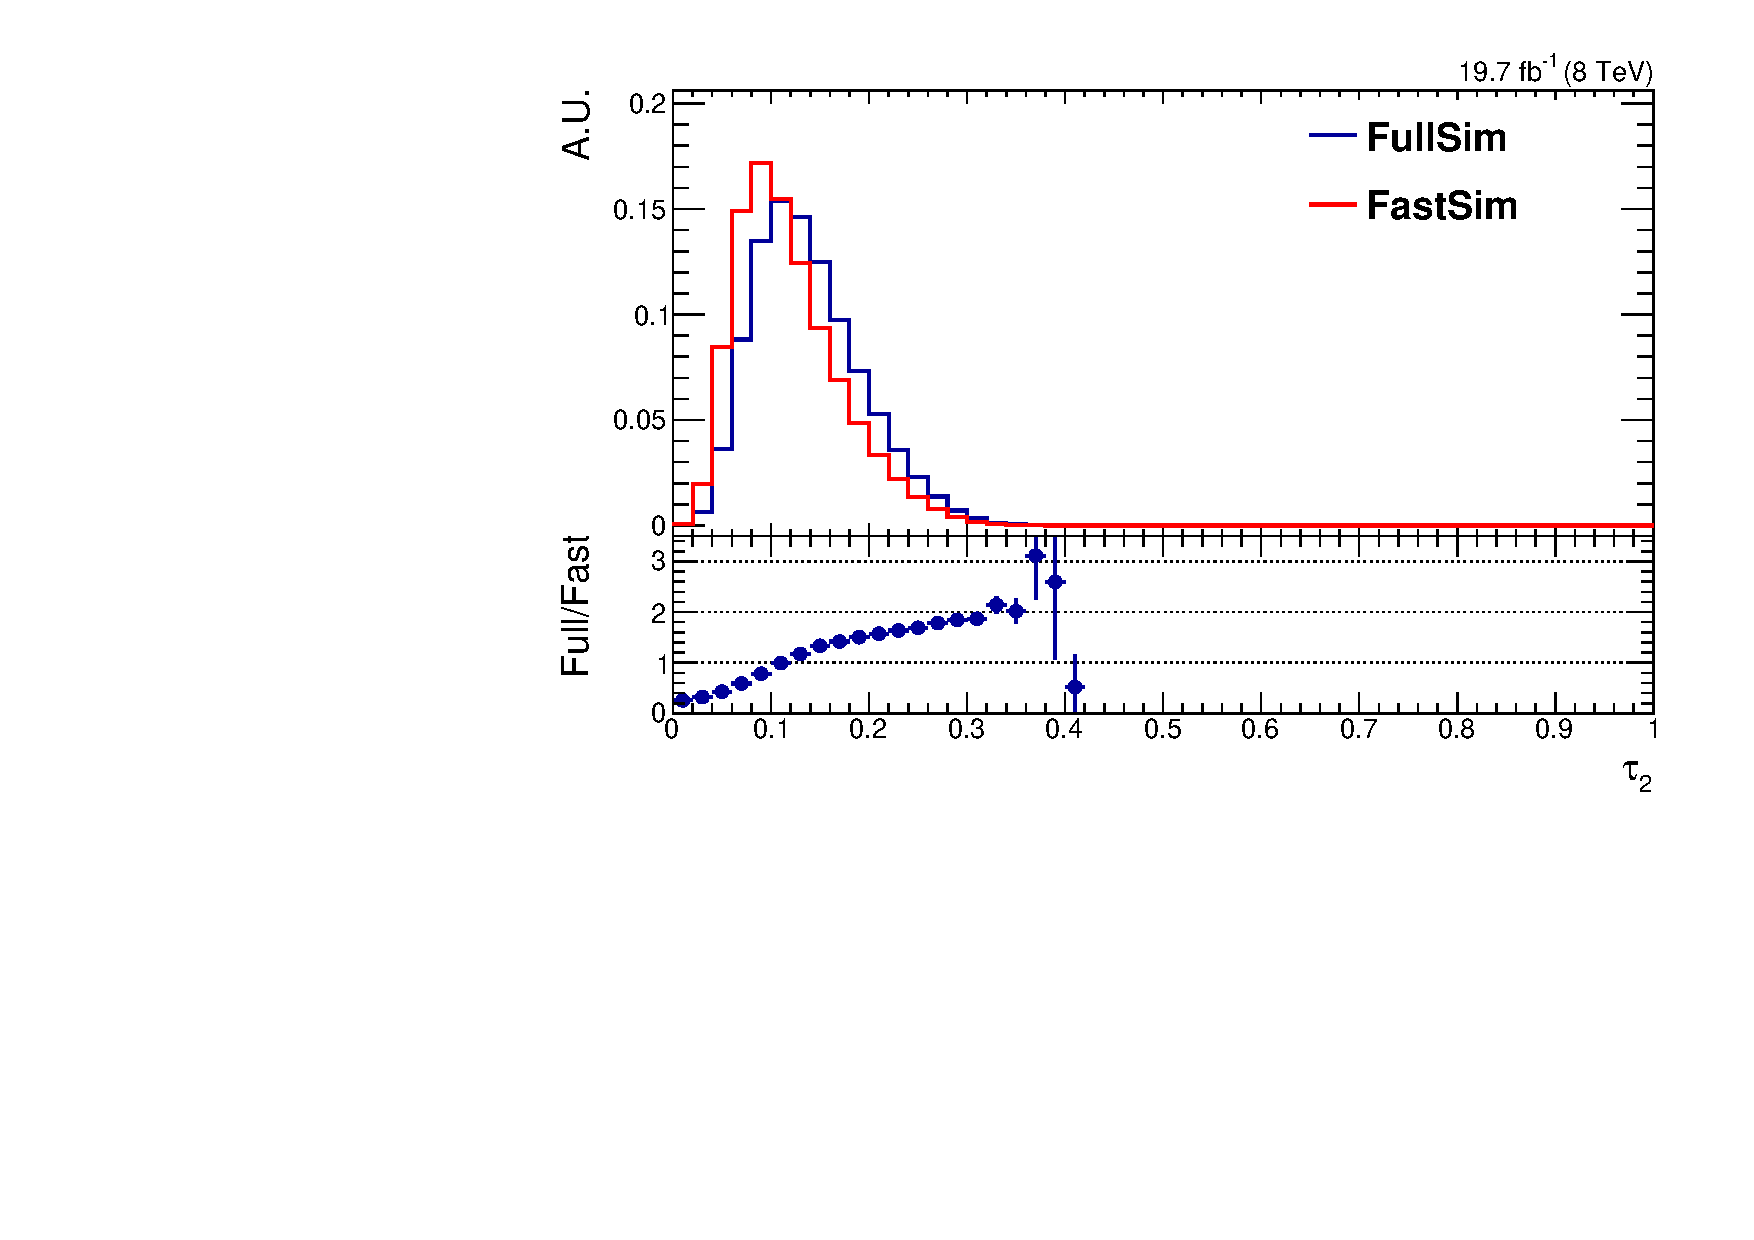
\includegraphics[width=0.49\textwidth]{figures/razor_wtag/FastFull_comparison_TTJets_tau2_masscut}
\caption{Distribution of $\tau_2$ before (left) and after (right) requiring the pruned CA8 jet to
lie within the $\W$ mass window, $70 < m_{\textrm{jet}} < 100$\GeV, for FastSim and FullSim
$t\bar{t}$.
\label{fig:FastFull_tau2}}
\end{figure}

\begin{figure}[p]
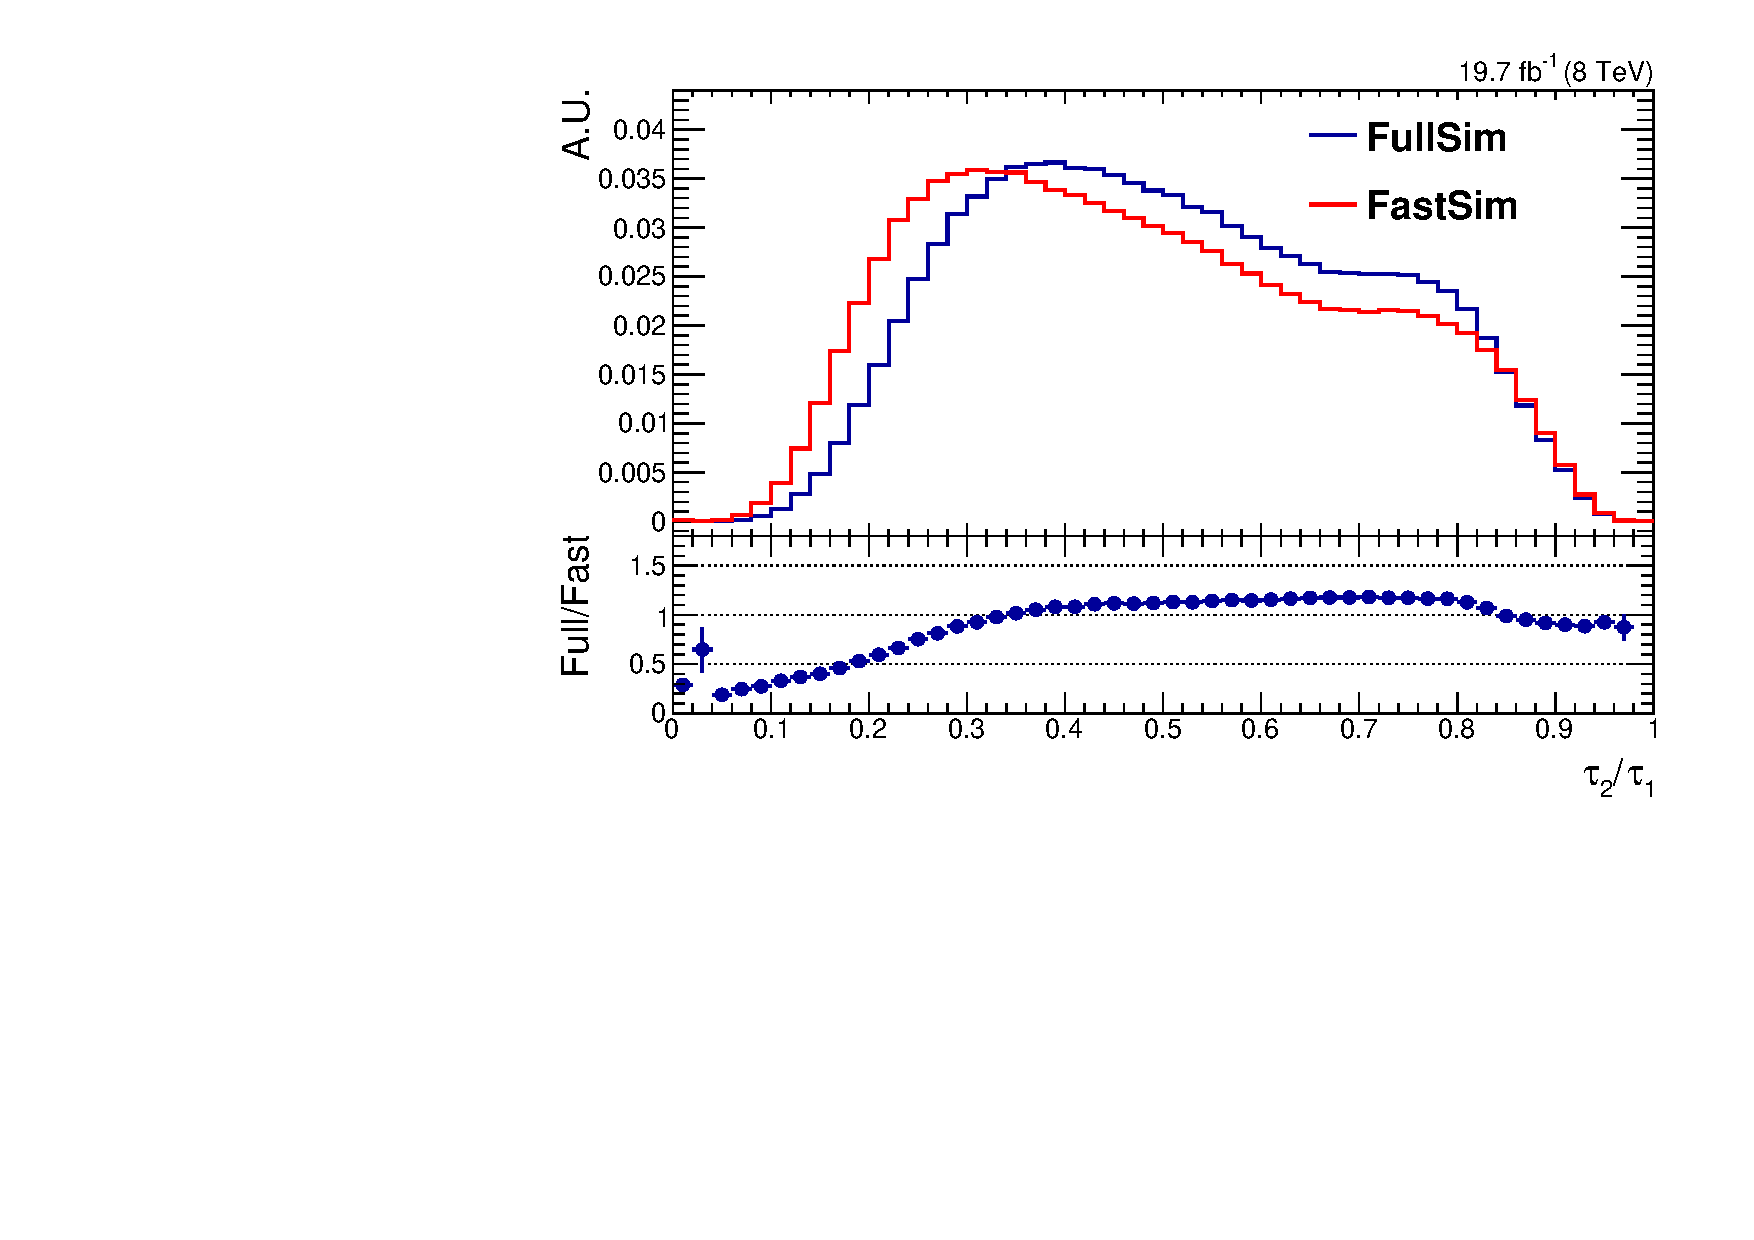
\includegraphics[width=0.49\textwidth]{figures/razor_wtag/FastFull_comparison_TTJets_tau21}
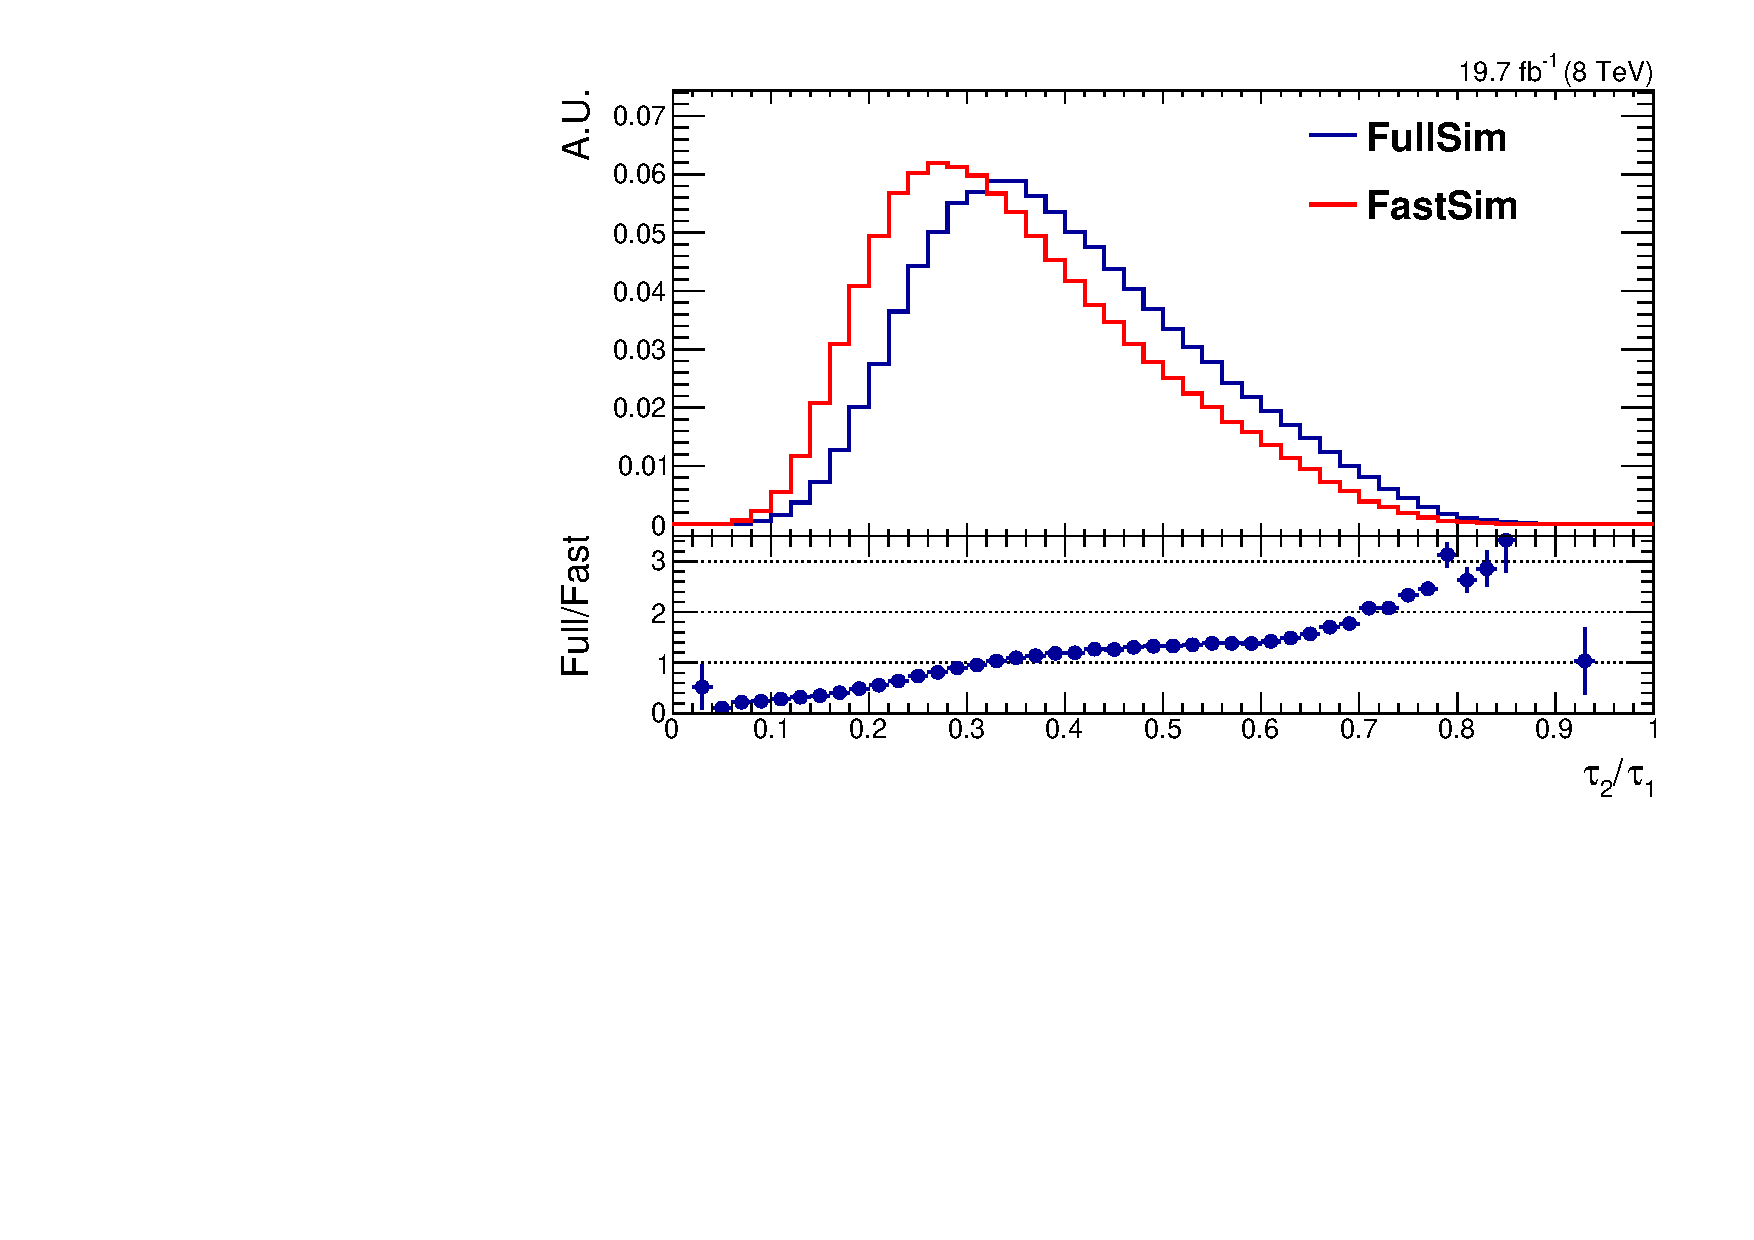
\includegraphics[width=0.49\textwidth]{figures/razor_wtag/FastFull_comparison_TTJets_tau21_masscut}
\caption{Distribution of $\tau_2/\tau_1$ before (left) and after (right) requiring the pruned CA8
jet to lie within the $\W$ mass window, $70 < m_{\textrm{jet}} < 100$\GeV, for FastSim and FullSim
$t\bar{t}$.
\label{fig:FastFull_tau21}}
\end{figure}

These figures also illustrate some of the features of the N-subjettiness variables.
Consider first the $\tau_1$ distribution in Fig.~\ref{fig:FastFull_tau1}. Without a jet mass
requirement, the distribution is quite broad and bimodal. Once the jet mass is required to
be consistent with the $\W$ boson mass, the lower part of the distribution disappears. This
illustrates that quark/gluon jets are expected to have only a single subjet, resulting in a small
$\tau_1$ value. For jets that result from the decay of a $\W$ boson, $\tau_1$ takes on a larger
value. 
This effect is not seen for the $\tau_2$ distributions (Fig.~\ref{fig:FastFull_tau2}), which is
expected because $\tau_2$ quantifies the compatibility with having two or fewer subjets. 
The ratio $\tau_2/\tau_1$, shown on Fig.~\ref{fig:FastFull_tau21}, also displays the
expected behaviour: the part of the distribution at high values is removed when requiring the jet
mass to be within the $\W$ mass window, and thus when selecting more jets with two-prong decays. 

The procedure to determine the $\W$ boson tagging efficiency for both FastSim and FullSim is the
following:
\begin{enumerate}
\item Filter the events at the generator level, requiring the presence of exactly one hadronically
decaying $\W$ boson. 
\item For the generated $\W$ boson, find the closest reconstructed CA8 jet, and require that it be
within $\Delta R = 0.8$ from the $\W$ boson. If no such jet exists, the event is discarded.  
\item Require that there be no (generator-level) $\cPqb$ quark from the top quark decay within the
cone of the selected CA8 jet. (We wish to select boosted $\W$ bosons only, not boosted top quarks.)
\item For the events that pass the above selection, consider the $\pt$ distribution of the CA8 jet
at two selection levels:
 \begin{itemize}
   \item no additional selection
   \item $70 < m_\textrm{jet} < 100$\GeV and $\tau_2/\tau_1 < 0.5$
 \end{itemize}
\item By dividing those \pt distributions we obtain the $\W$ boson tagging efficiency. 
\end{enumerate}
To derive the FullSim/FastSim scale factor for the $\W$ boson tagging efficiency, we divide the
efficiencies $\epsilon$ obtained in FullSim and FastSim:
\begin{equation}
SF_{\textrm{Full/Fast}}(\pt) =
\frac{\epsilon_{\textrm{FullSim}}(\pt)}{\epsilon_{\textrm{FastSim}}(\pt)}.
\end{equation}
A graphical representation of the $\W$ boson tag efficiency in FastSim and FullSim is shown on
Fig.~\ref{fig:boost_Wfullfast} for a fine and more coarse binning in CA8 jet \pt. The resulting
scale factor is shown for the final, coarse binning that will be used to rescale the signal
simulation. 
Table~\ref{tab:SF_FullFast} summarizes the $\W$ boson tag efficiency FullSim/FastSim scale factor
with its
statistical uncertainty.

\begin{figure}[htbp]
\centering
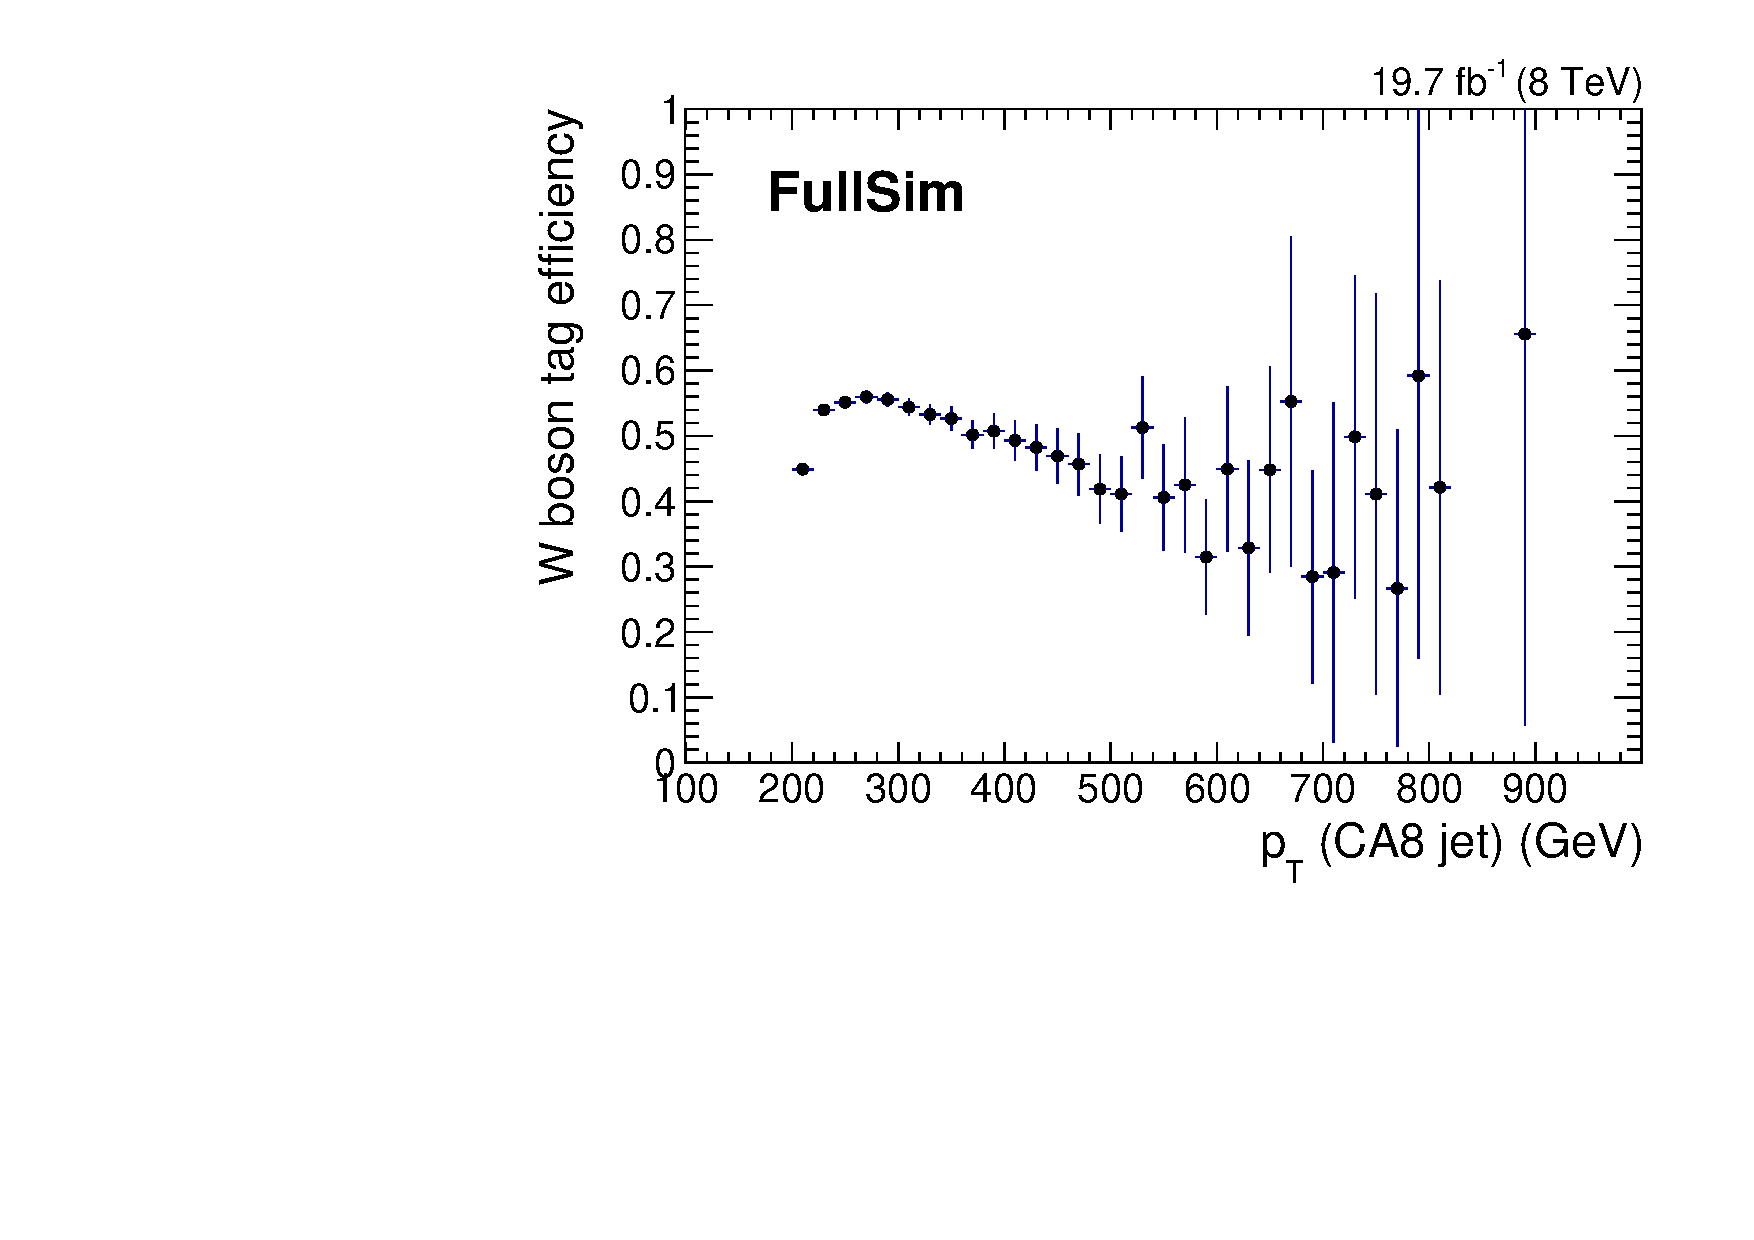
\includegraphics[width=0.48\textwidth]{figures/razor_wtag/Eff_ratio_tagged_all_FullSim_Thesis}
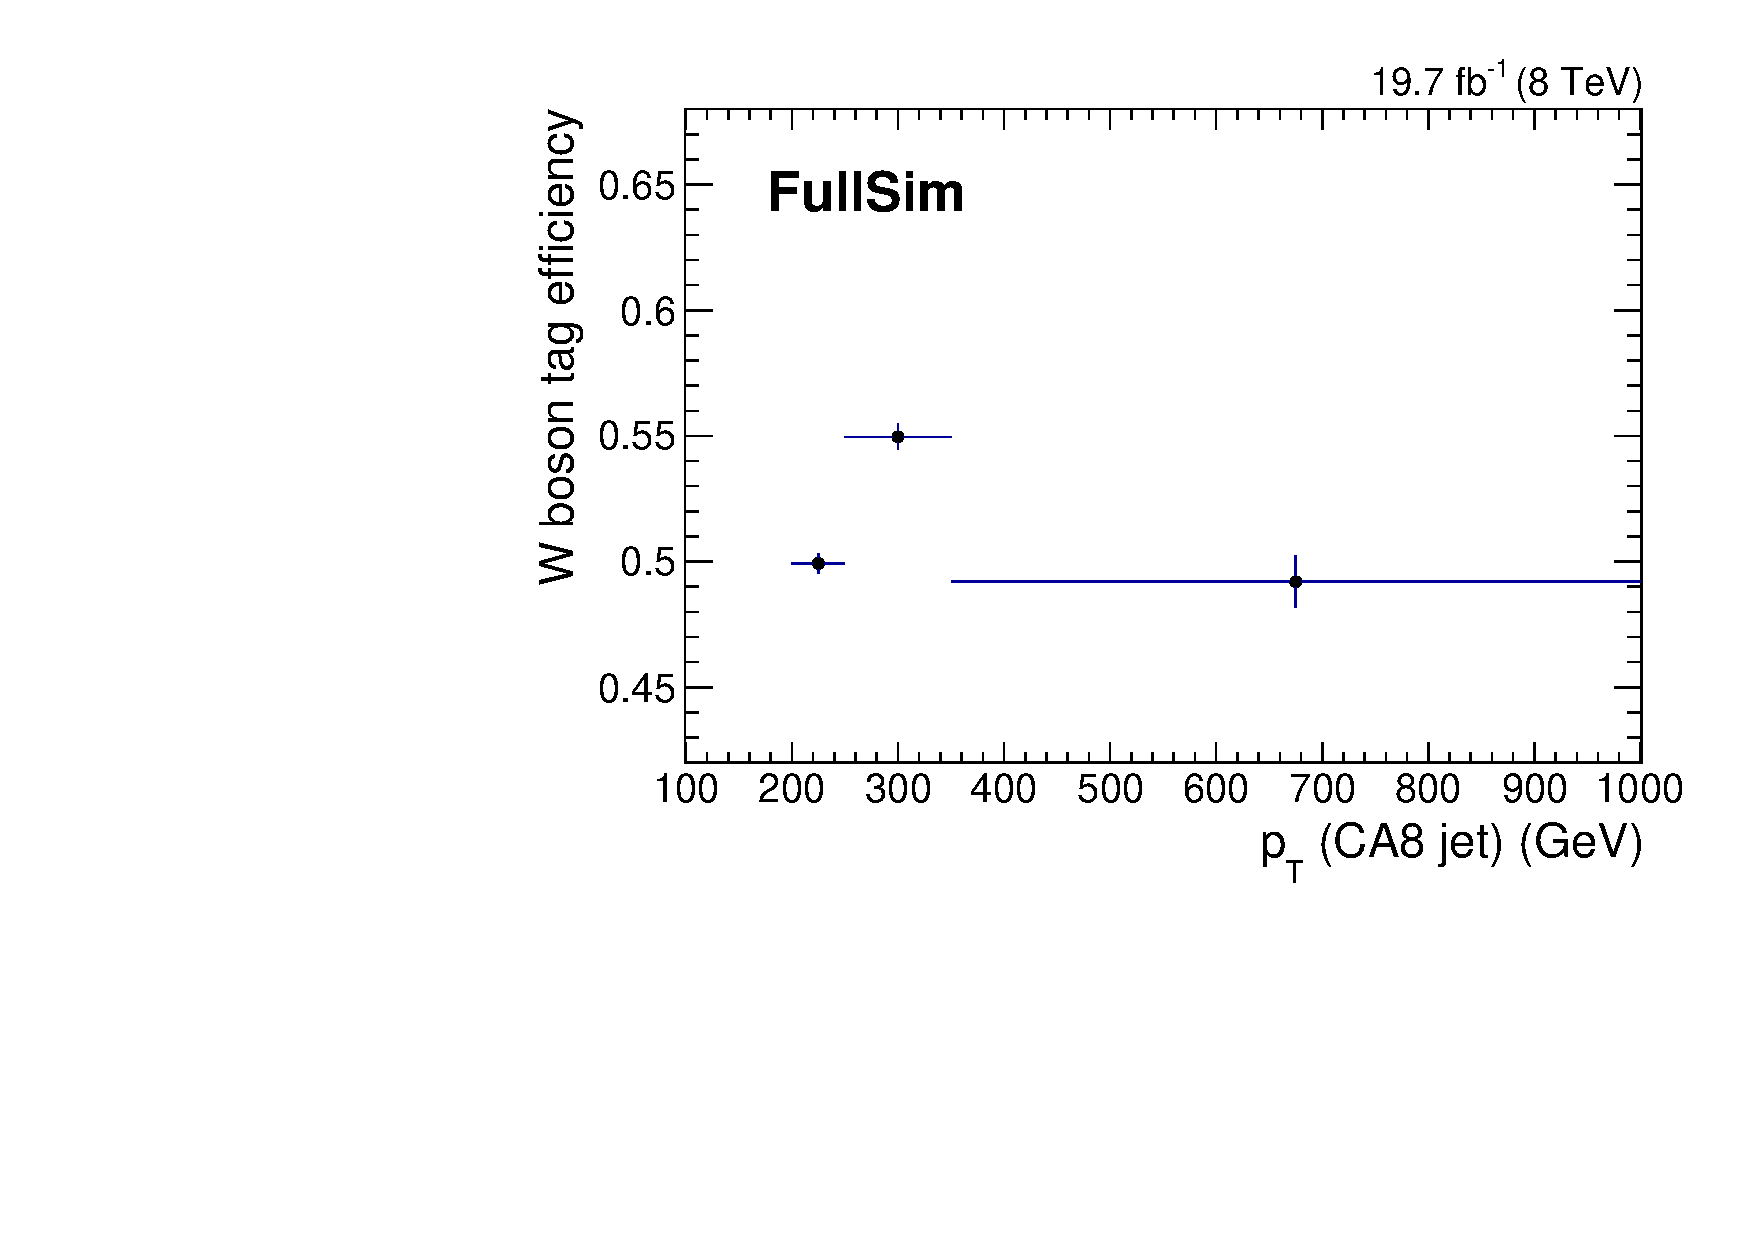
\includegraphics[width=0.48\textwidth]
{figures/razor_wtag/Eff_ratio_tagged_all_varbin_FullSim_Thesis}

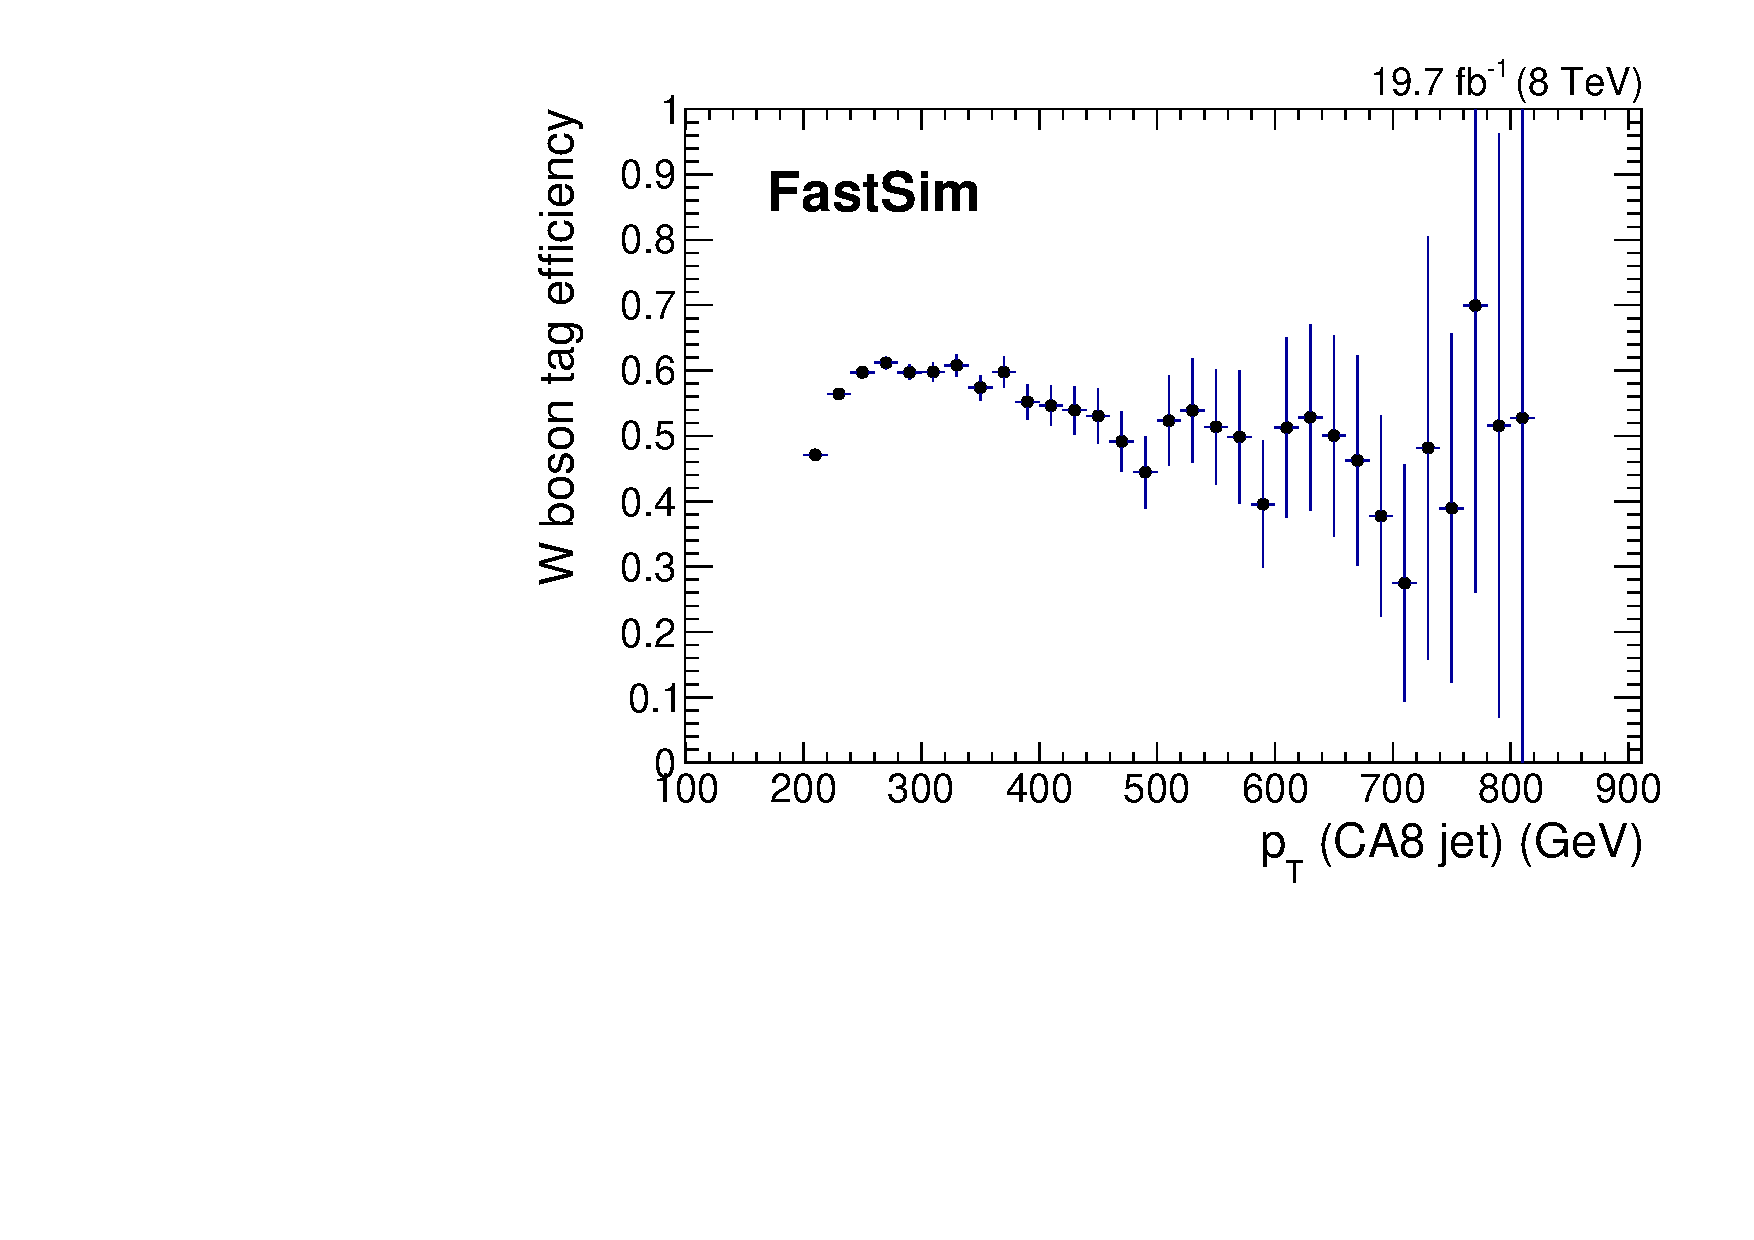
\includegraphics[width=0.48\textwidth]{figures/razor_wtag/Eff_ratio_tagged_all_FastSim_Thesis}
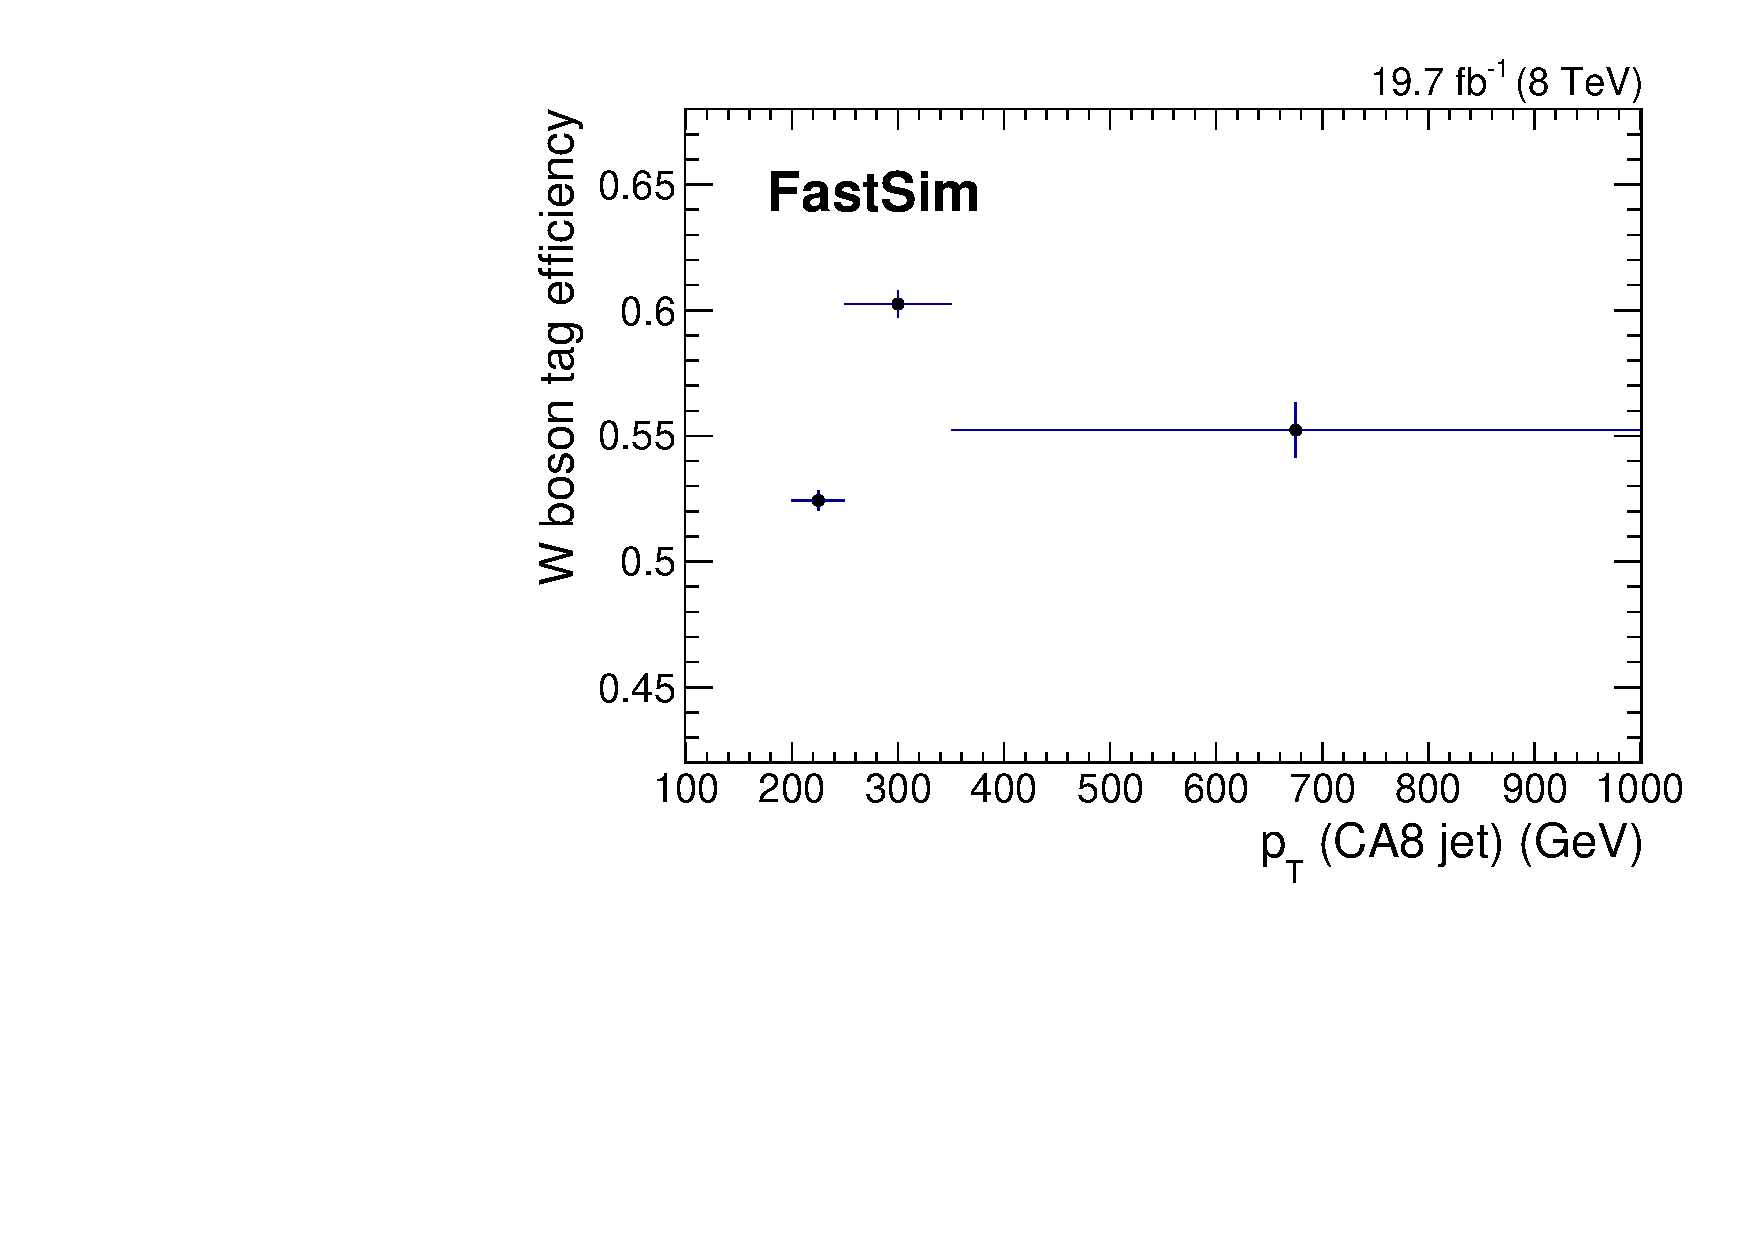
\includegraphics[width=0.48\textwidth]
{figures/razor_wtag/Eff_ratio_tagged_all_varbin_FastSim_Thesis}

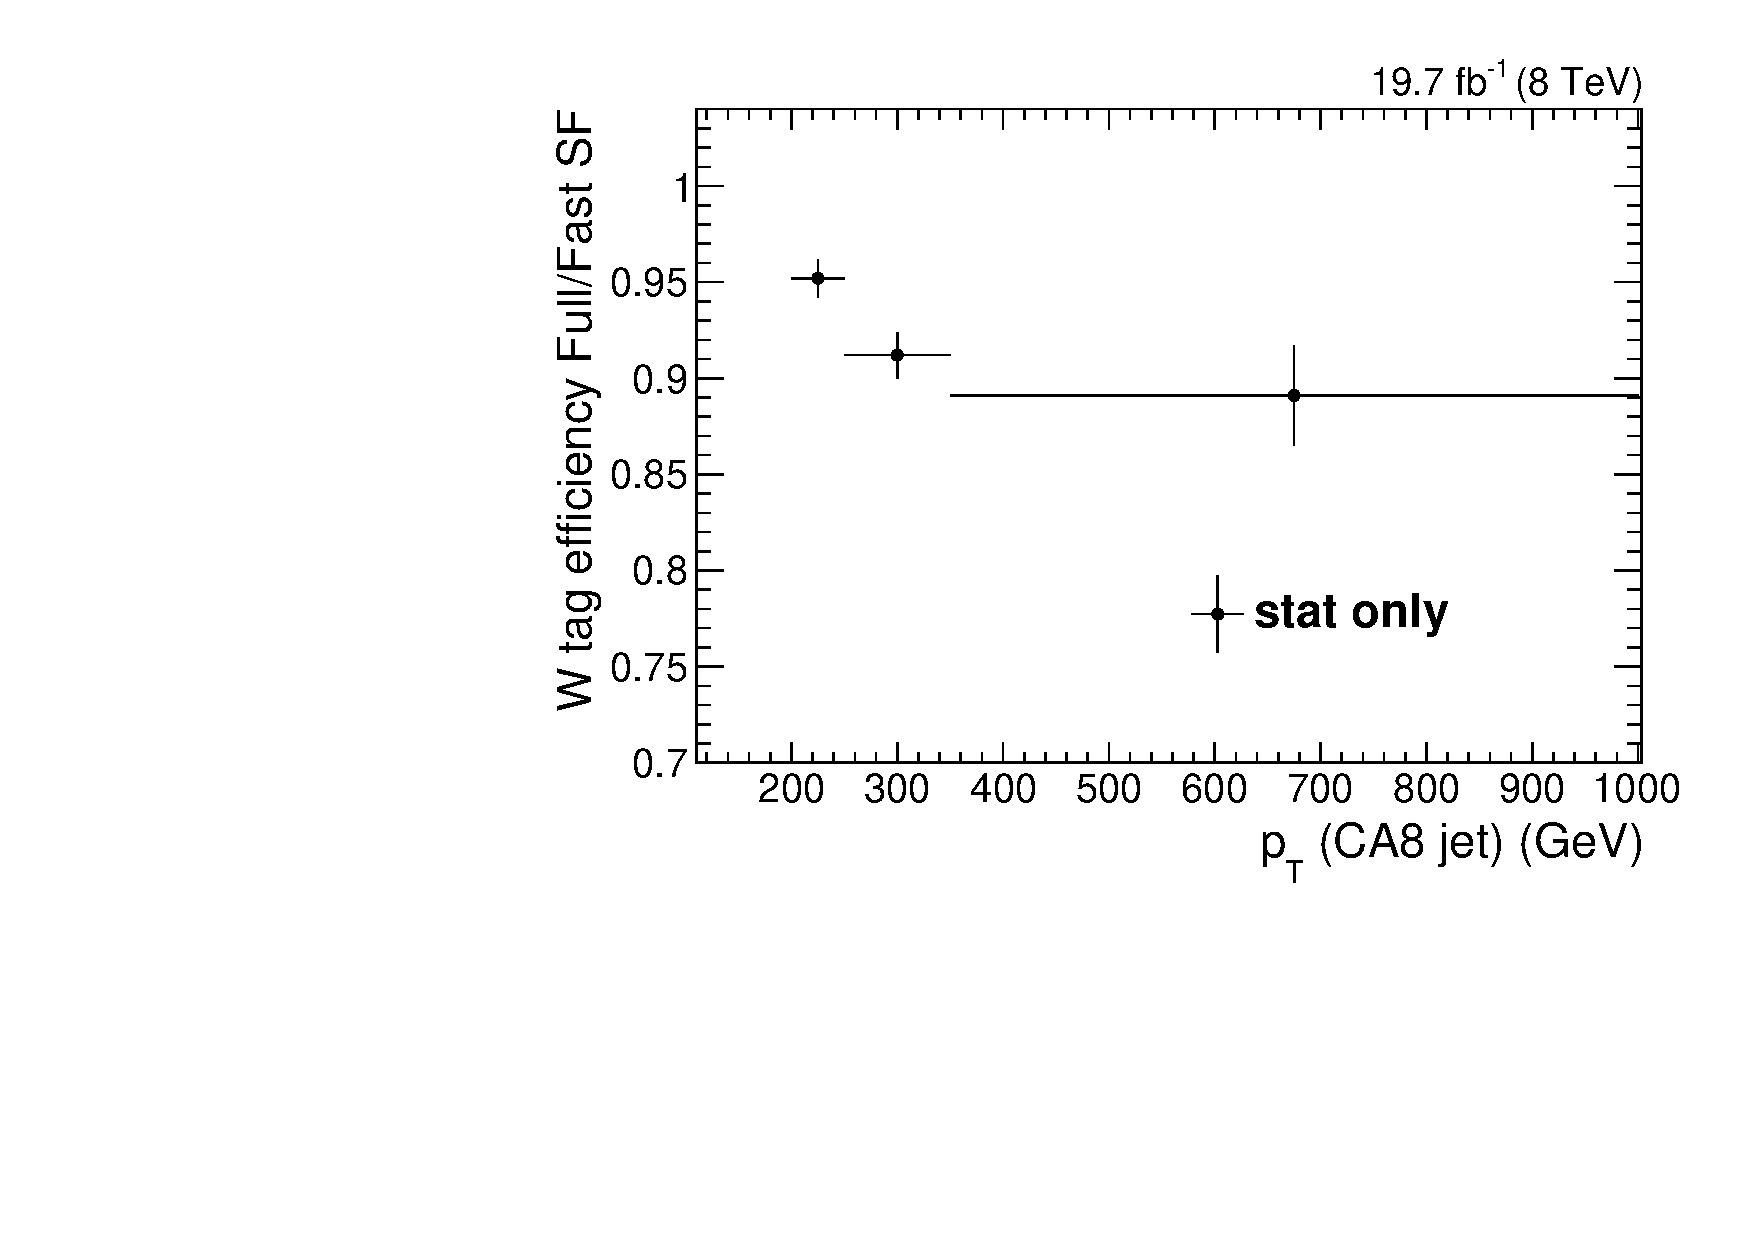
\includegraphics[width=0.6\textwidth]{figures/razor_wtag/SF_FullFast_Thesis}
\caption{[top] $\W$ boson tag efficiency versus CA8 jet \pt, with two different binnings, obtained
from FullSim $t\bar{t}$ events as described in the text. The shown uncertainties are statistical
only. 
[middle] $\W$ boson tag efficiency versus CA8 jet \pt, with two different binnings, obtained from
FastSim $t\bar{t}$ events as described in the text. The shown uncertainties are statistical only. 
[bottom] $\W$ boson tag FullSim/FastSim efficiency scale factor versus CA8 jet \pt. The shown
uncertainties are statistical only.
\label{fig:boost_Wfullfast}}
\end{figure}

\begin{table}[htpb]
\centering
\caption{Summary of FullSim/FastSim scale factor for the $\W$ tag efficiency.}
\vspace{1ex}
\begin{tabular}{c c}
\toprule
CA8 jet $\pt$ (\GeV) & $SF_{\textrm{Full/Fast}}$\\
\midrule
$[200 - 250[$ &  $0.952 \pm 0.010$ \\
$[250 - 350[$ &  $0.912 \pm 0.012$ \\
$[350 - ...]$ &  $0.891 \pm 0.026$ \\
\bottomrule
\end{tabular}
\label{tab:SF_FullFast}
\end{table}

%% ---------------------------------------------------------------------------------------------

\subsubsection{\texorpdfstring{$\W$}{W} boson tag fake rate scale factor \label{sec:wtag_fake_sf}}

The $\W$ boson tag fake rate scale factor is meant to correct processes that do not have
hadronically decaying $\W$ bosons in their final state. As the fake rate depends on the composition
of the sample, this scale factor has to be derived for each analysis separately. 
We will thus need to obtain a sample of events containing misidentified $\W$ boson jets to derive a
dedicated scale factor for the razor boost analysis. A multijet-enriched control region is defined,
using the following selection:
\begin{itemize}
\item no loose leptons, 
\item no $\cPqb$ tagged (CSVL) jets,
\item at least 3 AK5 jets,
\item at least one AK5 jet with $\pt>200$\GeV,
\item small minimum azimuthal angle between the \VEtmiss and the leading three jets, \\
$\Delta\phi_{min} < 0.3$.
\end{itemize}
This selection is similar to the baseline selection employed in the rest of the analysis. The
kinematic regime, and the composition of the sample will thus also be similar. The main difference
is that we have not applied any selection on the razor variables \mr or \rsq, in order to retain a
higher statistical power. 

To obtain the fake rates $\epsilon$ for $\W$ boson tagging we use the leading CA8 jet in each
event, and check whether it is tagged by the $\W$ boson tagger. After obtaining the
fake rates in both data and simulation, we compute the scale factor as their ratio,
\begin{equation}
SF_\textrm{Wtag}^\textrm{fake}(\pt) =
\frac{\epsilon^{\textrm{data}}(\pt)}{\epsilon^{\textrm{simulation}}(\pt)}.
\end{equation} 
In the calculation of the uncertainties on this scale factor we include the statistical uncertainty,
as well as the trigger efficiency and jet energy scale uncertainties for both AK5 and CA8 jets. 
All three uncertainties are varied up (down) at the same time to get the overall up (down)
systematic  uncertainty.
The fake rate in data and simulation, as well as the resulting $\W$ boson tag fake rate scale factor
are shown in Fig.~\ref{fig:boost_wfake}. As we can see from the figure, there is a drop in the scale
factor just above a \pt of 300\GeV. This is a result of a residual mismodelling of the trigger
efficiency. 

%\textcolor{red}{TODO: add more information on this "wiggle", perhaps in an appendix.}

\begin{figure}[htbp]
\centering
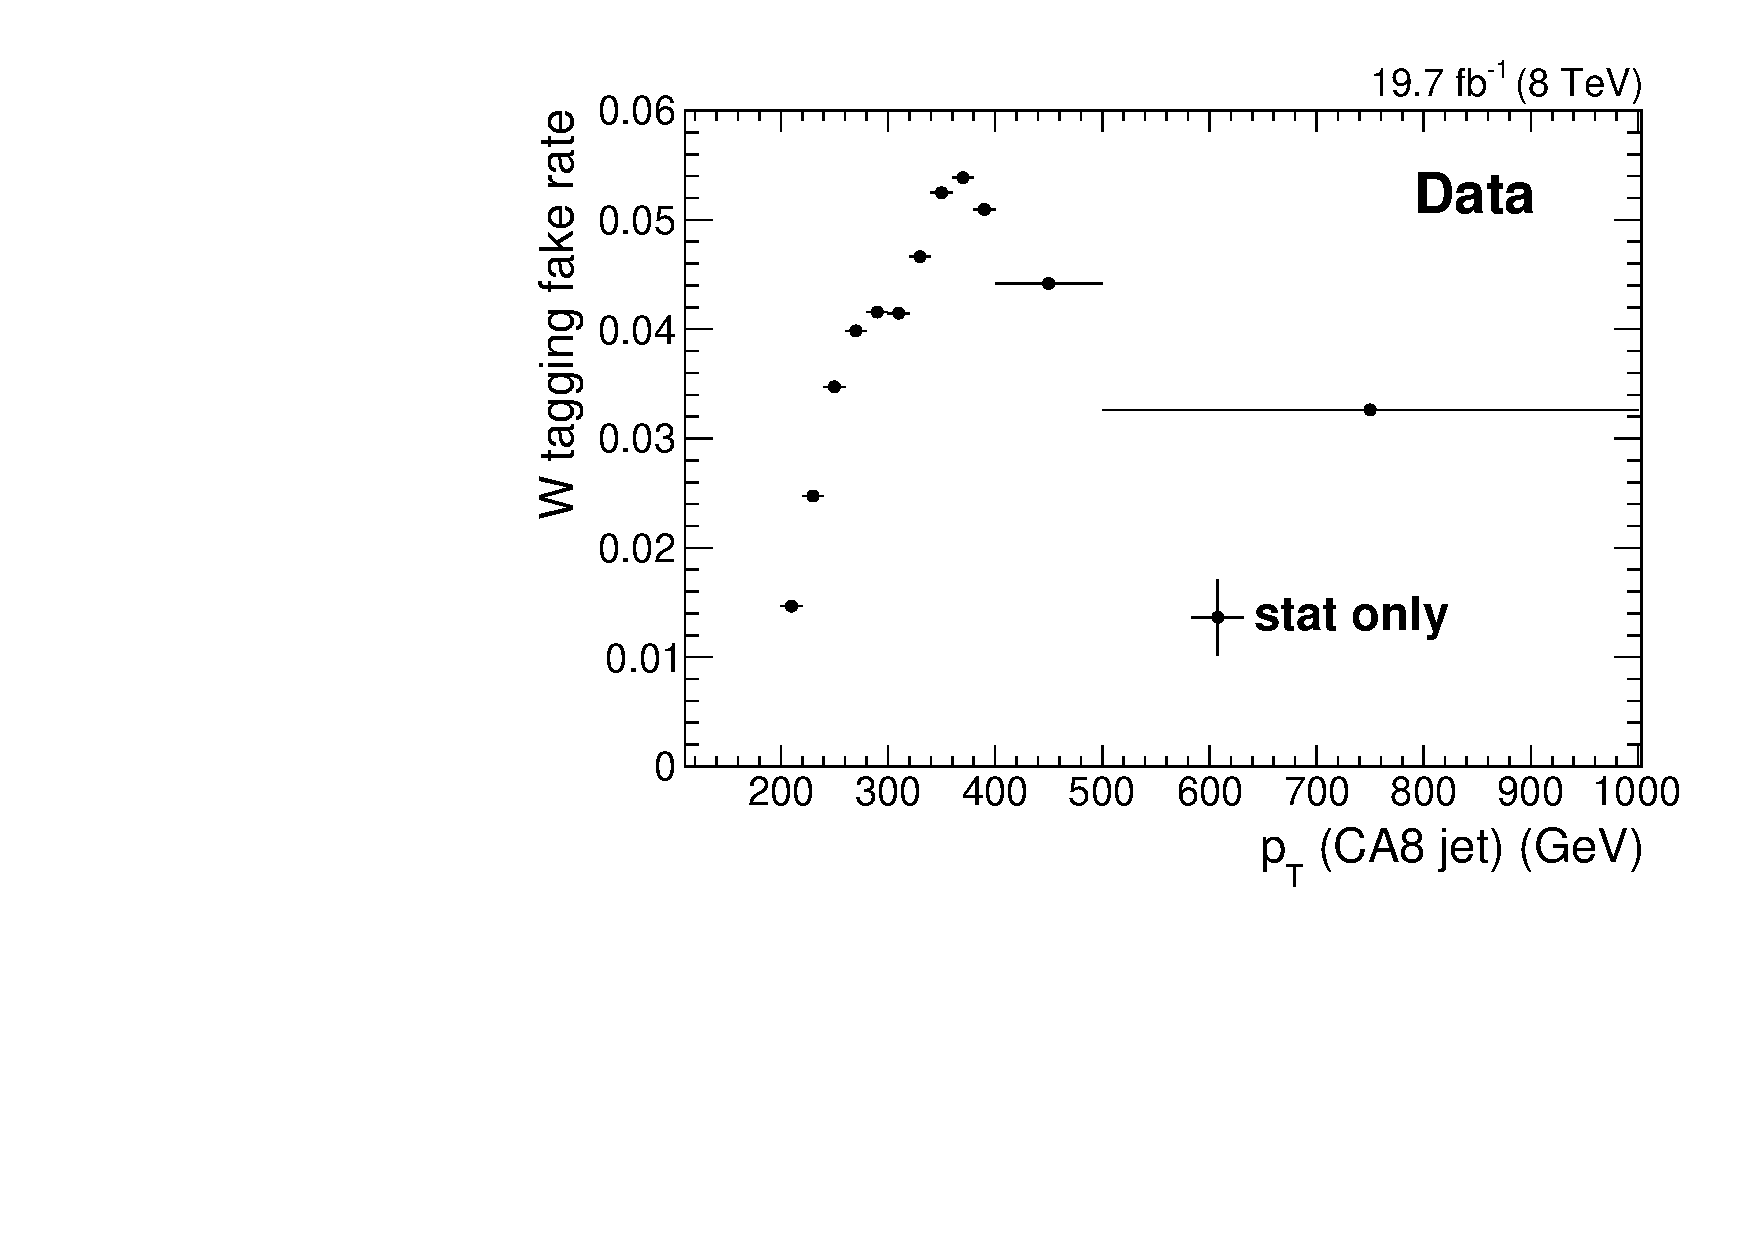
\includegraphics[width=0.6\textwidth]{figures/razor_wtag/Eff_Data_ratio_pt_tagged_all_Data_Thesis}

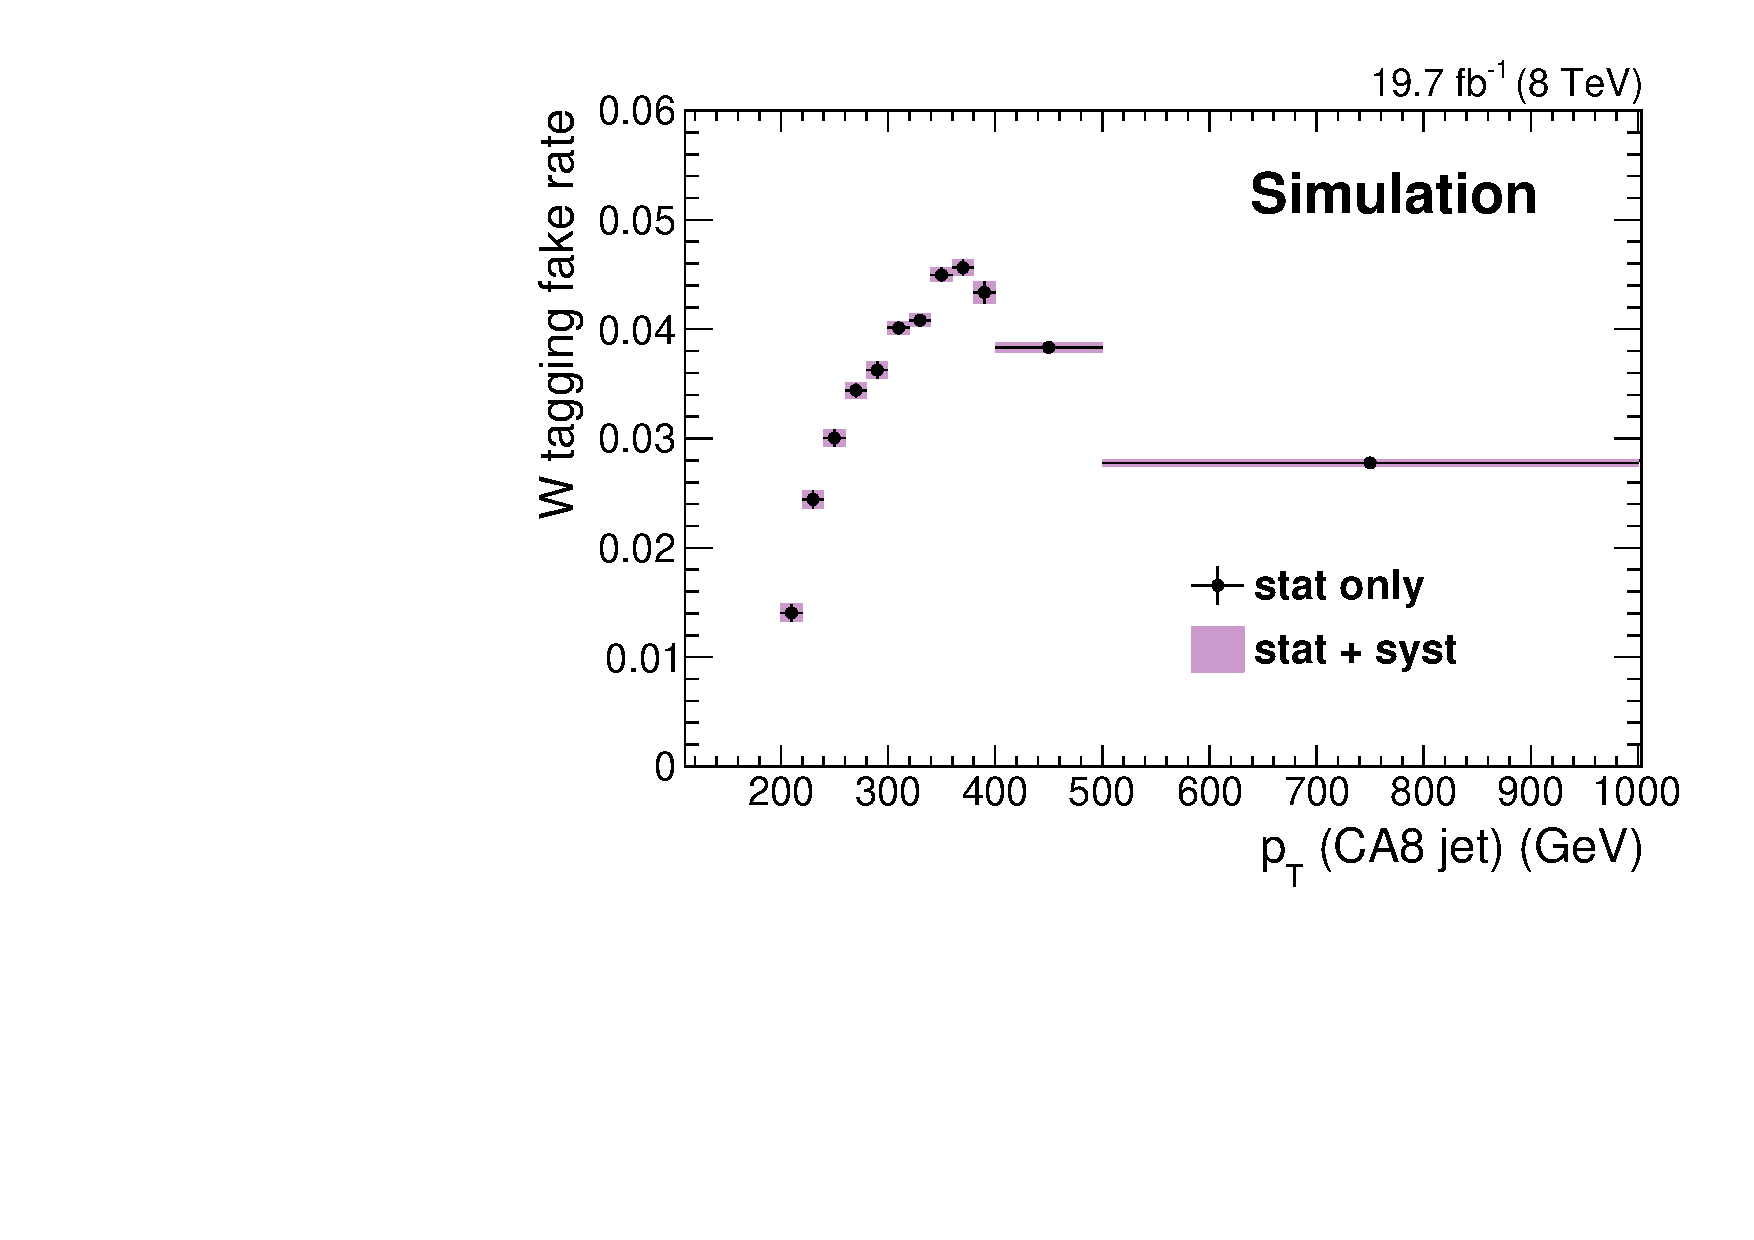
\includegraphics[width=0.6\textwidth]{figures/razor_wtag/Eff_MC_ratio_pt_tagged_all_MC_Thesis}

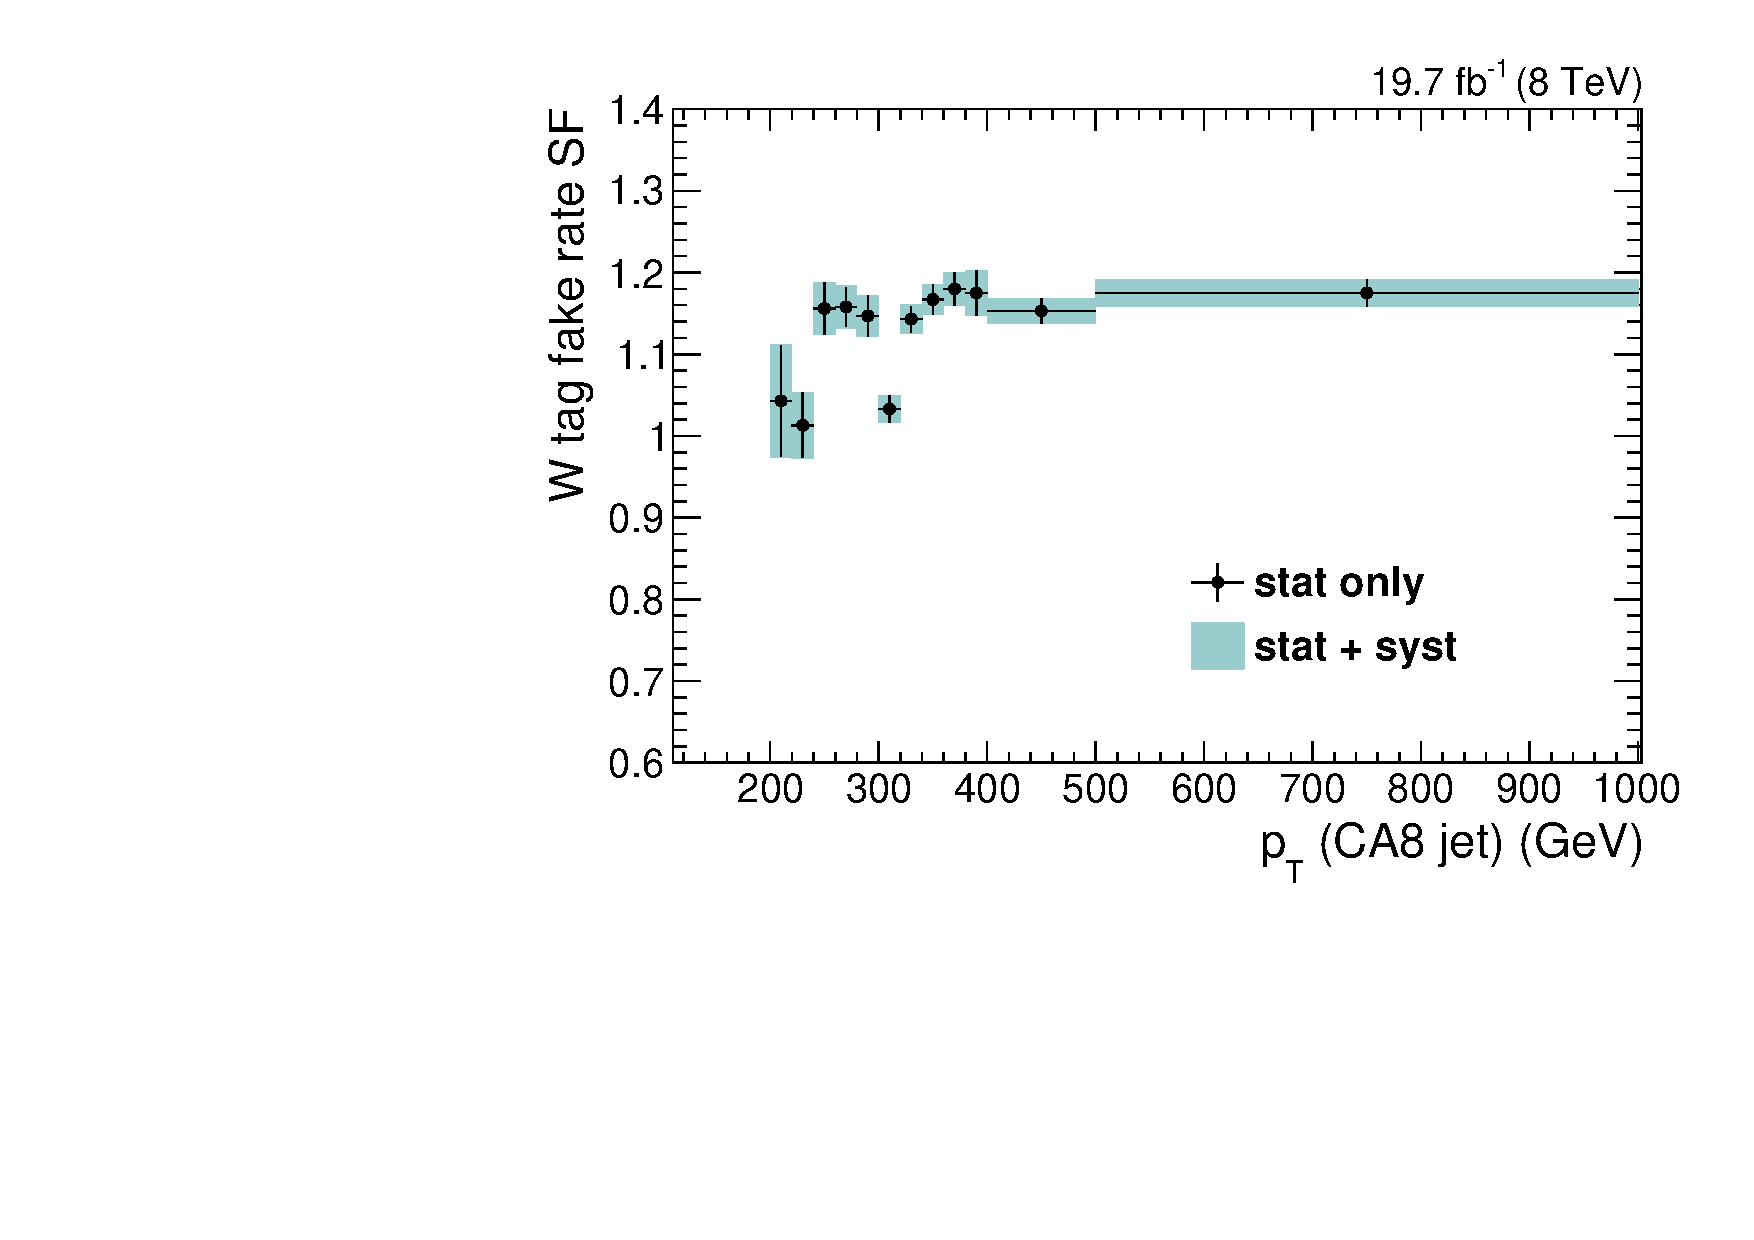
\includegraphics[width=0.6\textwidth]{figures/razor_wtag/SF_Wfake_Thesis}
\caption{[top] Misidentification probability according to $\W$ tagging for a CA8 jet versus
jet \pt obtained from a multijet-enriched control region in data as described in the text. The shown
uncertainties are statistical only. 
[middle] $\W$ boson tag fake rate obtained from simulation. The uncertainty band includes
statistical and systematic uncertainties.
[bottom] Scale factor for $\W$ tag fake rate versus CA8 jet \pt obtained from a
multijet-enriched control region as described in the text. The uncertainty band includes
statistical and systematic uncertainties.
\label{fig:boost_wfake}}
\end{figure}

The $\W$ boson tag fake rate scale factor is applied in the $S$ and $T$ region, as is the case for
the $\W$ boson tag efficiency scale factor. It is applied to all simulated samples without real
hadronically decaying $\W$ bosons, such as multijet production, $W(\rightarrow\ell\nu)$+jets,
$\cPZ/\gamma^*(\rightarrow\ell\ell)$+jets, etcetera. 

%% ---------------------------------------------------------------------------------------------

\subsubsection{\texorpdfstring{$\W$}{W} boson mass-tag fake rate scale factor
\label{sec:wmasstag_fake_sf}}

This scale factor corresponds to the $\W$ boson mass-tagging definition, which will be used in the
$W$ control region. As we will see further, the $W$ region is dominated by leptonically decaying
$\W$ bosons. The mass-tagged jet, therefore, originates from a quark or gluon jet, and is a
misidentified $\W$ boson jet. For this reason we will derive the scale factor for the $\W$ boson
mass-tag fake rate from the same multijet-enriched region as was used to derive the scale factor for
the $\W$ boson tag fake rate. The same method as before is applied, the only difference being
the use of the $\W$ boson mass-tag definition instead of the $\W$ boson tag definition. 

The resulting scale factor, $SF_\textrm{Wmasstag}^\textrm{fake}$, is again a function of the CA8
jet \pt, and will be applied to all simulated samples in the $W$ region.
Figure~\ref{fig:boost_wmasstag} shows the $\W$ boson mass-tag fake rate in data and
simulation, and the corresponding scale factor versus CA8 jet \pt. The scale factor with
associated statistical and systematic uncertainties is listed in Table~\ref{tab:SF_Wmass}. The
systematic uncertainty includes the trigger efficiency uncertainty and the uncertainty on the jet
energy scale corrections. 
The drop in the scale factor just above a \pt of 300\GeV is also visible here. 

\begin{table}[htbp]
\centering
\caption{$\W$ boson mass-tag fake rate scale factor, binned in $\pt$. The breakdown in statistical
and systematic uncertainties is shown.  \label{tab:SF_Wmass}}
\vspace{1ex}
\begin{tabular}{c c}
\toprule
CA8 jet \pt (\GeV) & $SF_{\W\textrm{masstag}}^\textrm{fake}$ \\
\midrule
$[200 - 220[$ & $1.144 \pm 0.050 \,\textrm{(stat)} \pm 0.012 \,\textrm{(sys)}$ \\
$[220 - 240[$ & $1.118 \pm 0.028 \,\textrm{(stat)} \pm 0.024 \,\textrm{(sys)}$ \\
$[240 - 260[$ & $1.193 \pm 0.024 \,\textrm{(stat)} \pm 0.008 \,\textrm{(sys)}$ \\
$[260 - 280[$ & $1.250 \pm 0.018 \,\textrm{(stat)} \pm 0.015 \,\textrm{(sys)}$ \\
$[280 - 300[$ & $1.273 \pm 0.017 \,\textrm{(stat)} \pm 0.021 \,\textrm{(sys)}$ \\
$[300 - 320[$ & $1.126 \pm 0.013 \,\textrm{(stat)} \pm 0.010 \,\textrm{(sys)}$ \\
$[320 - 340[$ & $1.199 \pm 0.012 \,\textrm{(stat)} \pm 0.017 \,\textrm{(sys)}$ \\
$[340 - 360[$ & $1.298 \pm 0.013 \,\textrm{(stat)} \pm 0.007 \,\textrm{(sys)}$ \\
$[360 - 380[$ & $1.327 \pm 0.016 \,\textrm{(stat)} \pm 0.008 \,\textrm{(sys)}$ \\
$[380 - 400[$ & $1.339 \pm 0.025 \,\textrm{(stat)} \pm 0.007 \,\textrm{(sys)}$ \\
$[400 - 500[$ & $1.339 \pm 0.012 \,\textrm{(stat)} \pm 0.005 \,\textrm{(sys)}$ \\
$[500 - ...]$ & $1.370 \pm 0.011 \,\textrm{(stat)} \pm 0.001 \,\textrm{(sys)}$ \\
\bottomrule
\end{tabular}
\end{table}

\begin{figure}[htbp]
\centering
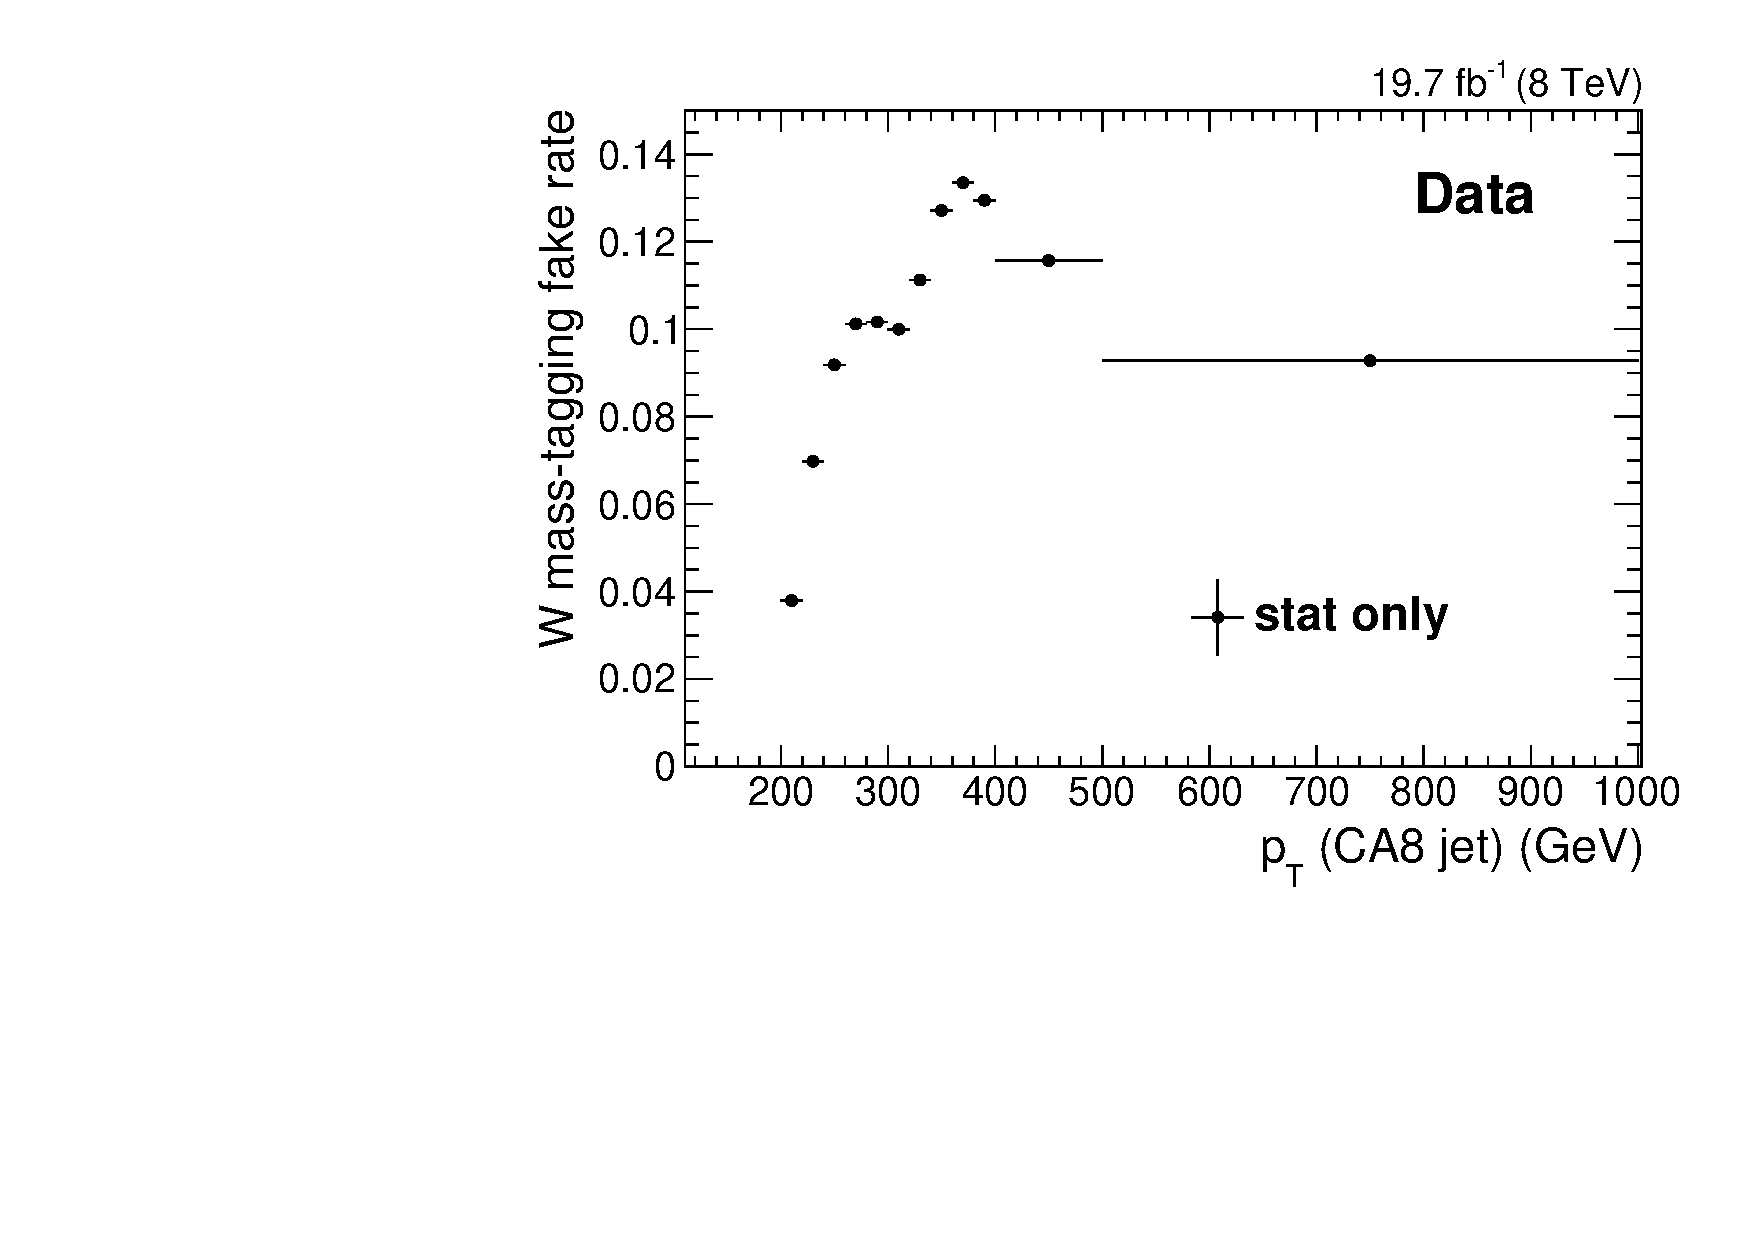
\includegraphics[width=0.6\textwidth]{figures/razor_wtag/Eff_Data_ratio_pt_Wmass_all_Data_Thesis}

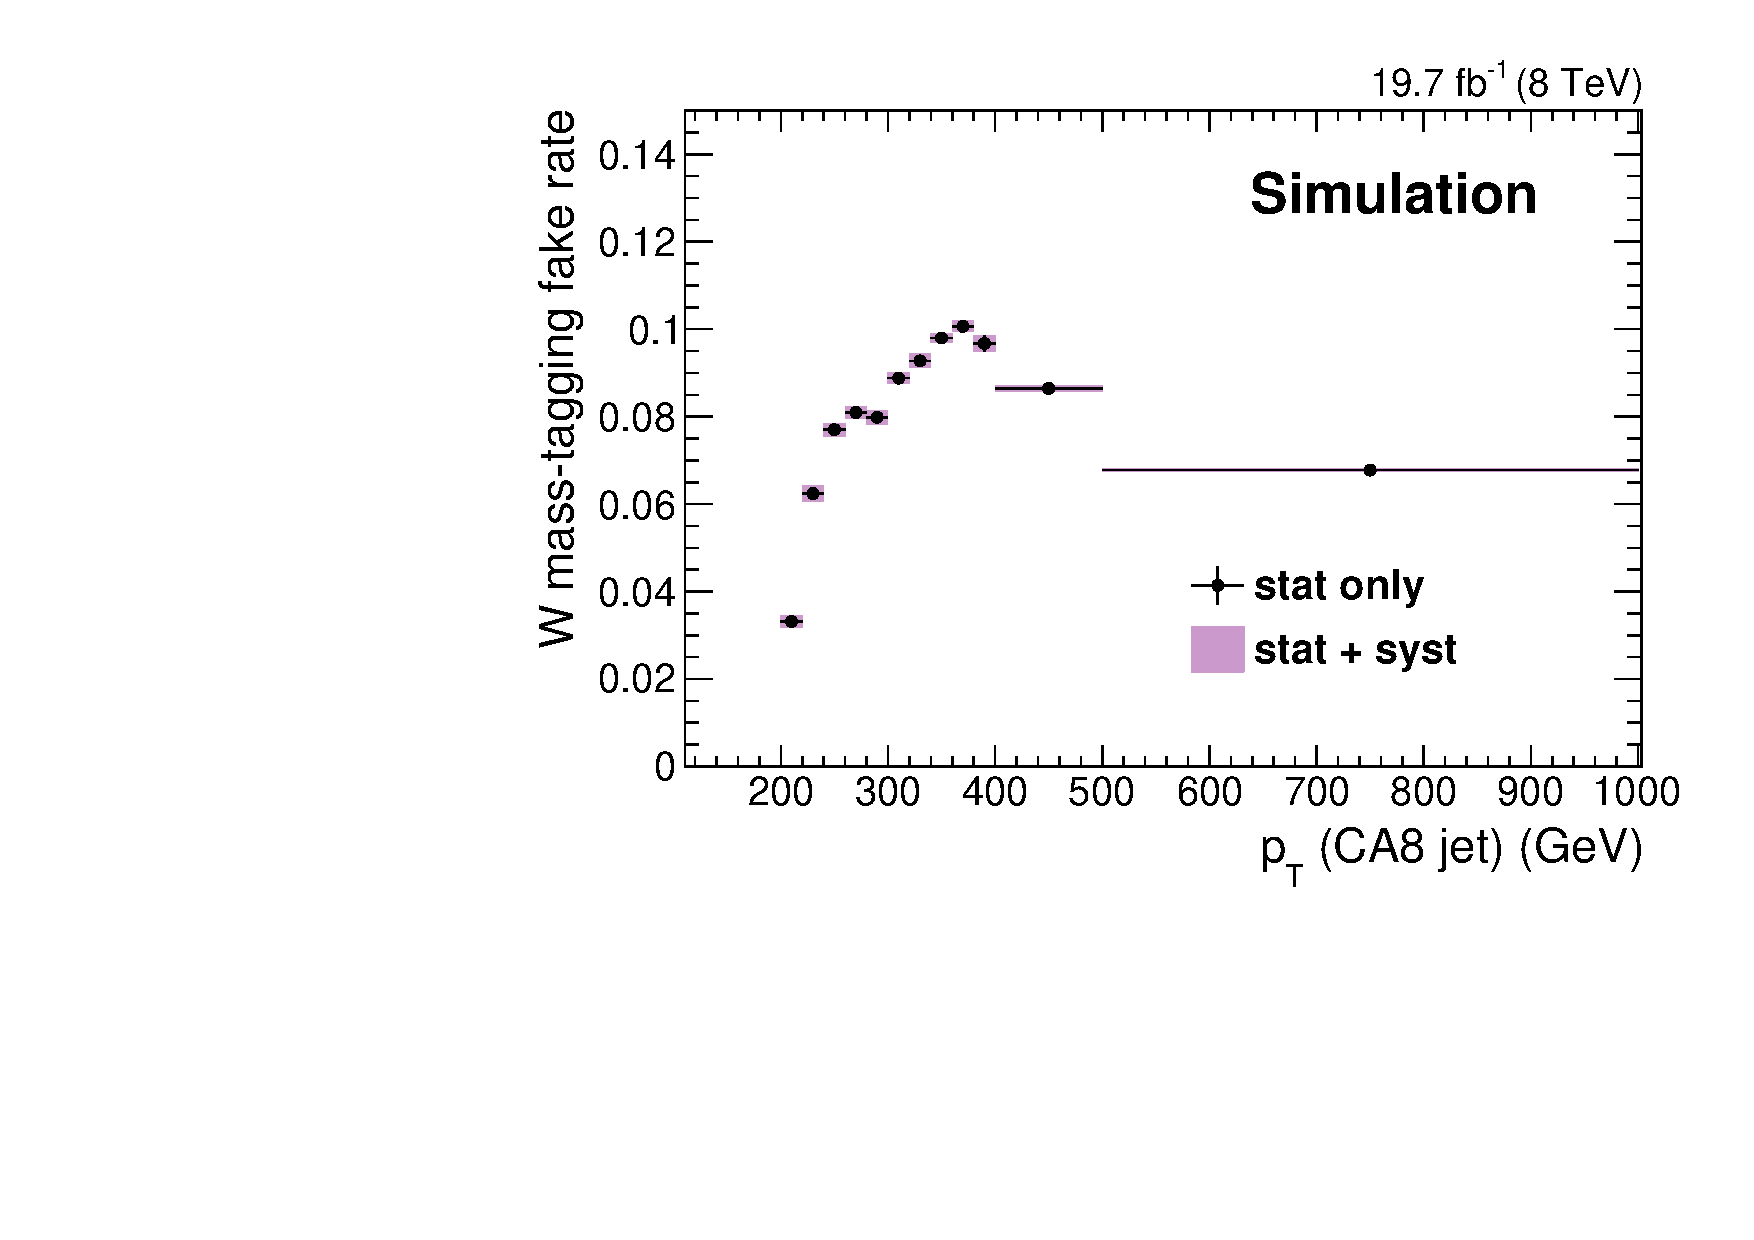
\includegraphics[width=0.6\textwidth]{figures/razor_wtag/Eff_MC_ratio_pt_Wmass_all_MC_Thesis}

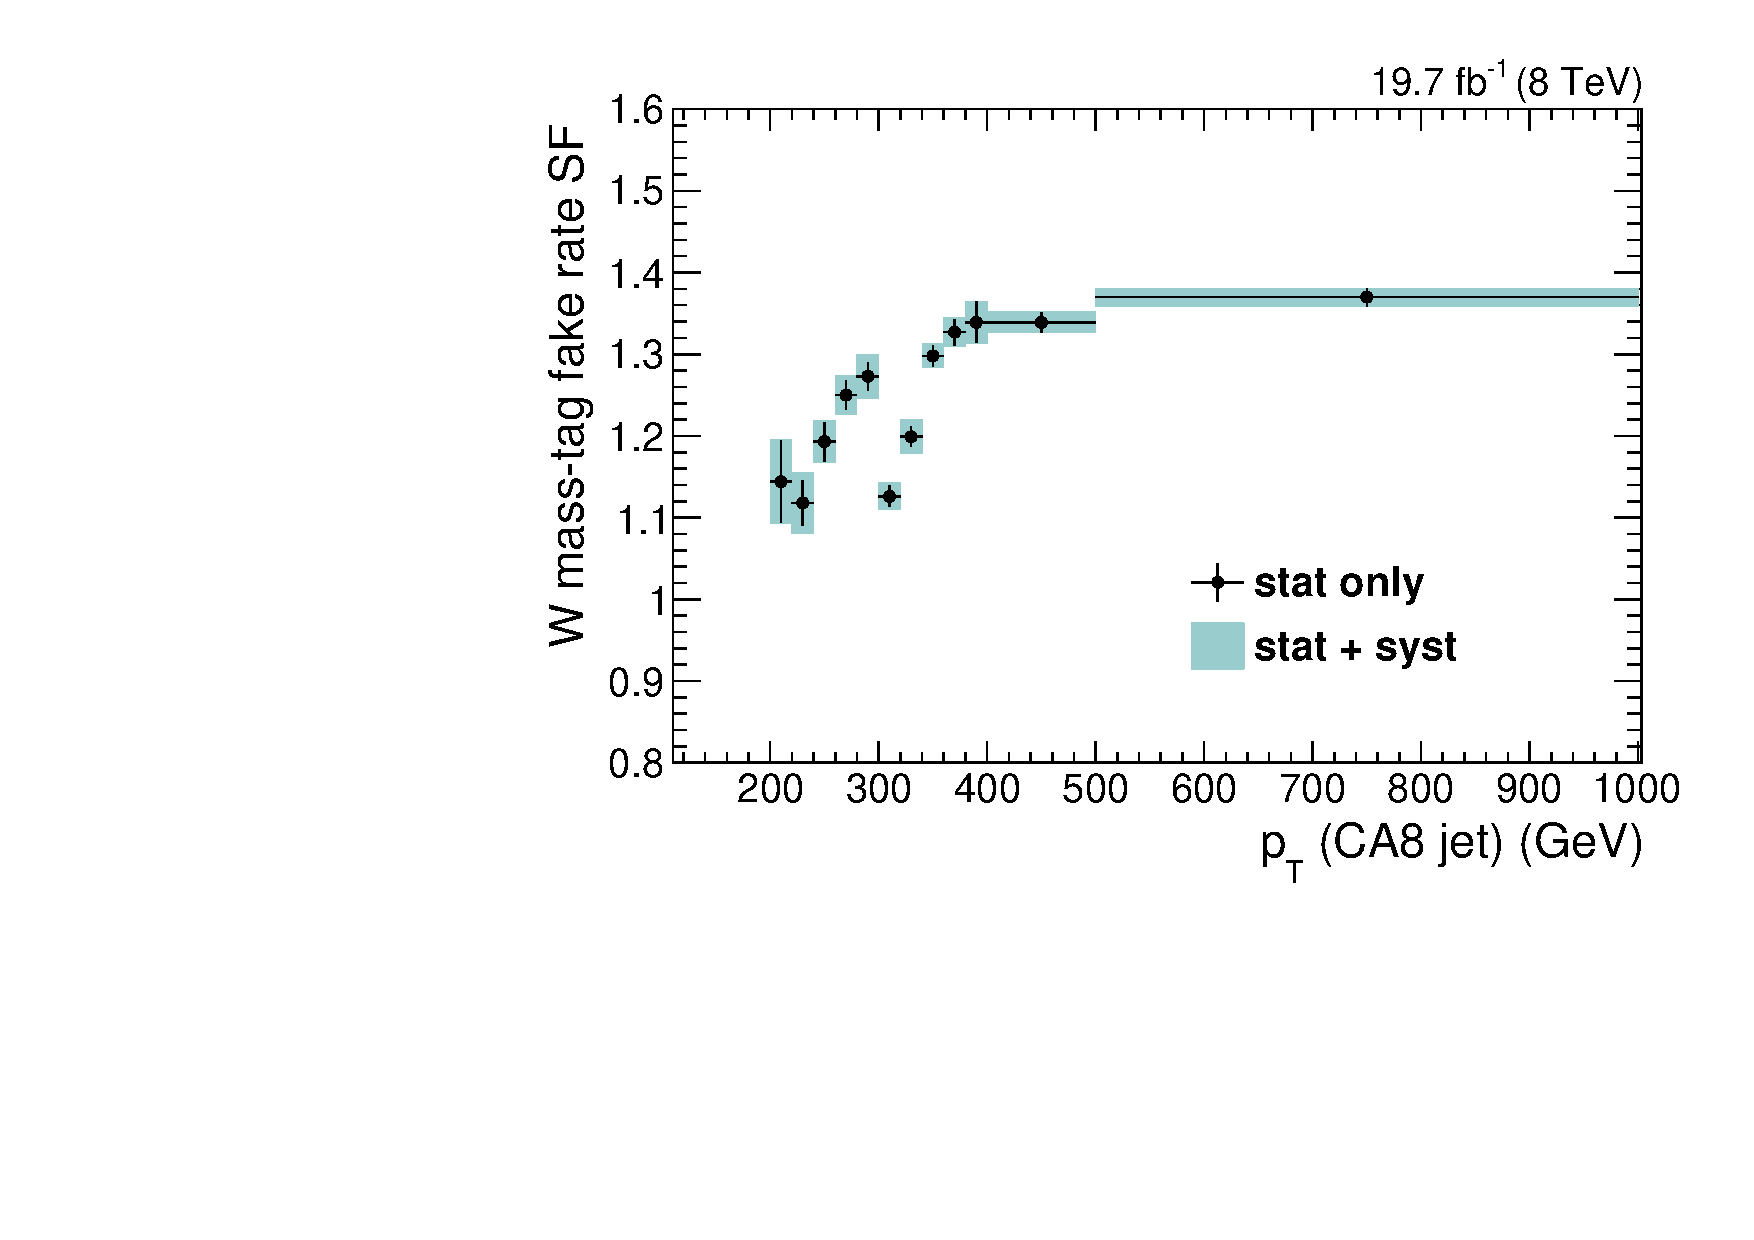
\includegraphics[width=0.6\textwidth]{figures/razor_wtag/SF_Wmass_Thesis}
\caption{[top] Misidentification probability according to $\W$ mass-tagging for a CA8 jet versus
jet \pt obtained from a multijet-enriched control region in data as described in the text. The shown
uncertainties are statistical only.
[middle] $\W$ boson mass-tag fake rate according to simulation. The uncertainty band includes
statistical and systematic uncertainties.
[bottom] Scale factor for $\W$ mass-tag fake rate versus CA8 jet \pt obtained from a
multijet-enriched control region as described in the text. The uncertainty band includes
statistical and systematic uncertainties.
\label{fig:boost_wmasstag}}
\end{figure}

%% ---------------------------------------------------------------------------------------------

\subsubsection{\texorpdfstring{$\W$}{W} boson anti-tag fake rate scale factor
\label{sec:wantitag_fake_sf}}

This scale factor corresponds to the $\W$ boson anti-tagging definition, which will be used in the
$Q$ control region. This region is dominated by QCD multijet production. Consequently, the $\W$
anti-tagged jet originates from a quark/gluon jet and is a misidentified $\W$ boson jet. Once
more, we use the same procedure and the multijet-enriched region as for the $\W$ boson tag fake
rate scale factor.

The $\W$ boson anti-tag fake rate scale factor, $SF_\textrm{Wantitag}^\textrm{fake}$, will be
applied to all simulated samples in the $Q$ region. 
Figure~\ref{fig:boost_wantitag} shows the $\W$ boson anti-tag fake rate in data and
simulation, and the corresponding scale factor versus CA8 jet \pt. As before, we observe a drop in
the scale factor just above a \pt of 300\GeV. The scale factor, and breakdown of statistical and
systematic uncertainties, is listed in Table~\ref{tab:SF_Wantitagging}. The included systematic
uncertainties are those stemming from the trigger efficiency and jet energy scale corrections. 


\begin{table}[htbp]
\centering
\caption{$\W$ boson anti-tag fake rate scale factor, binned in $\pt$. The uncertainties are broken
down in their statistical and systematic component. \label{tab:SF_Wantitagging}}
\vspace{1ex}
\begin{tabular}{c c}
\toprule
CA8 jet \pt $(\GeV)$ & $SF_{\W \textrm{antitag}}^\textrm{fake}$ \\
\midrule
$[200 - 220[$ & $1.217 \pm 0.072 \,\textrm{(stat)} \pm 0.032 \,\textrm{(sys)}$ \\
$[220 - 240[$ & $1.186 \pm 0.037 \,\textrm{(stat)} \pm 0.046 \,\textrm{(sys)}$ \\
$[240 - 260[$ & $1.216 \pm 0.033 \,\textrm{(stat)} \pm 0.011 \,\textrm{(sys)}$ \\
$[260 - 280[$ & $1.319 \pm 0.024 \,\textrm{(stat)} \pm 0.019 \,\textrm{(sys)}$ \\
$[280 - 300[$ & $1.479 \pm 0.022 \,\textrm{(stat)} \pm 0.037 \,\textrm{(sys)}$ \\
$[300 - 320[$ & $1.203 \pm 0.017 \,\textrm{(stat)} \pm 0.015 \,\textrm{(sys)}$ \\
$[320 - 340[$ & $1.244 \pm 0.016 \,\textrm{(stat)} \pm 0.026 \,\textrm{(sys)}$ \\
$[340 - 360[$ & $1.409 \pm 0.019 \,\textrm{(stat)} \pm 0.015 \,\textrm{(sys)}$ \\
$[360 - 380[$ & $1.448 \pm 0.022 \,\textrm{(stat)} \pm 0.020 \,\textrm{(sys)}$ \\
$[380 - 400[$ & $1.472 \pm 0.033 \,\textrm{(stat)} \pm 0.014 \,\textrm{(sys)}$ \\
$[400 - 500[$ & $1.487 \pm 0.017 \,\textrm{(stat)} \pm 0.012 \,\textrm{(sys)}$ \\
$[500 - ...]$ & $1.505 \pm 0.014 \,\textrm{(stat)} \pm 0.004 \,\textrm{(sys)}$ \\
\bottomrule
\end{tabular}
\end{table}


\begin{figure}[htbp]
\centering
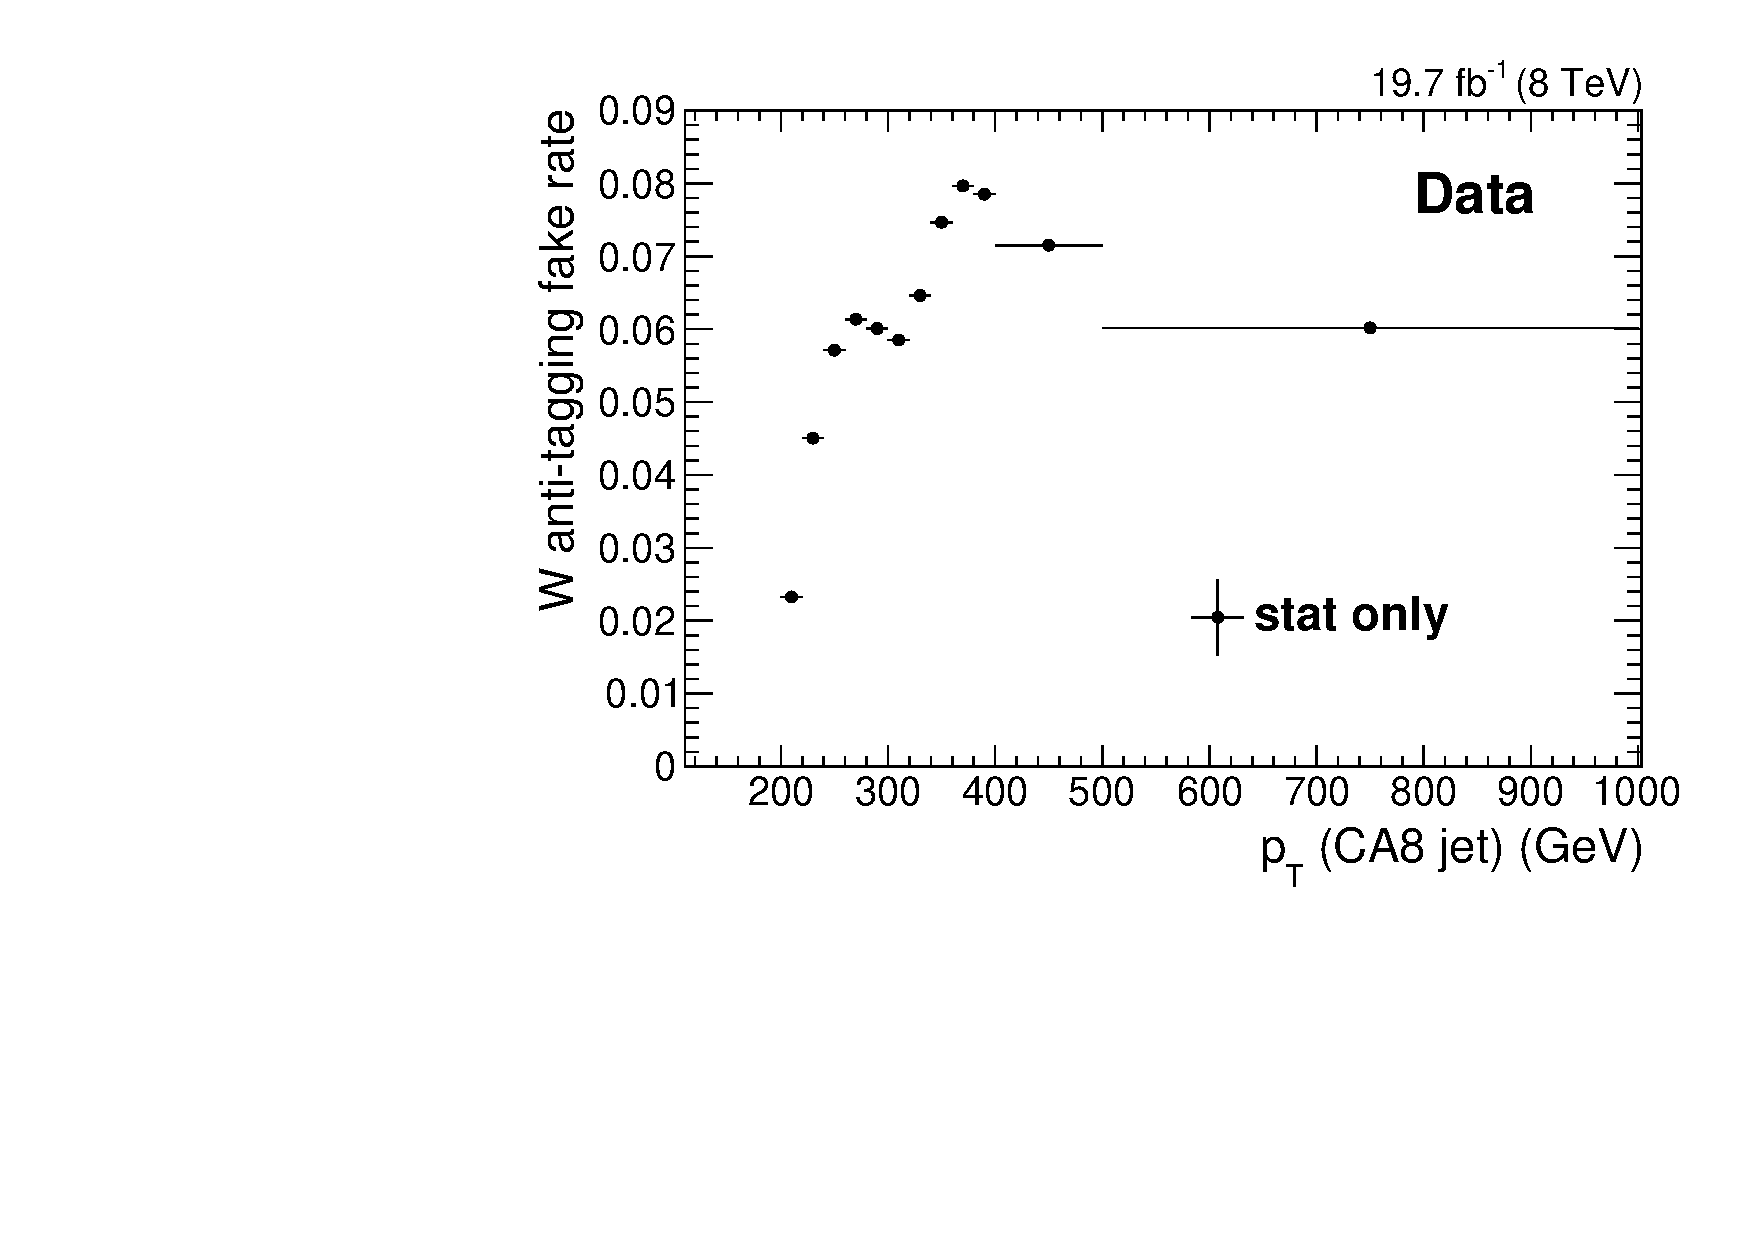
\includegraphics[width=0.6\textwidth]
{figures/razor_wtag/Eff_Data_ratio_pt_antitagged_all_Data_Thesis}

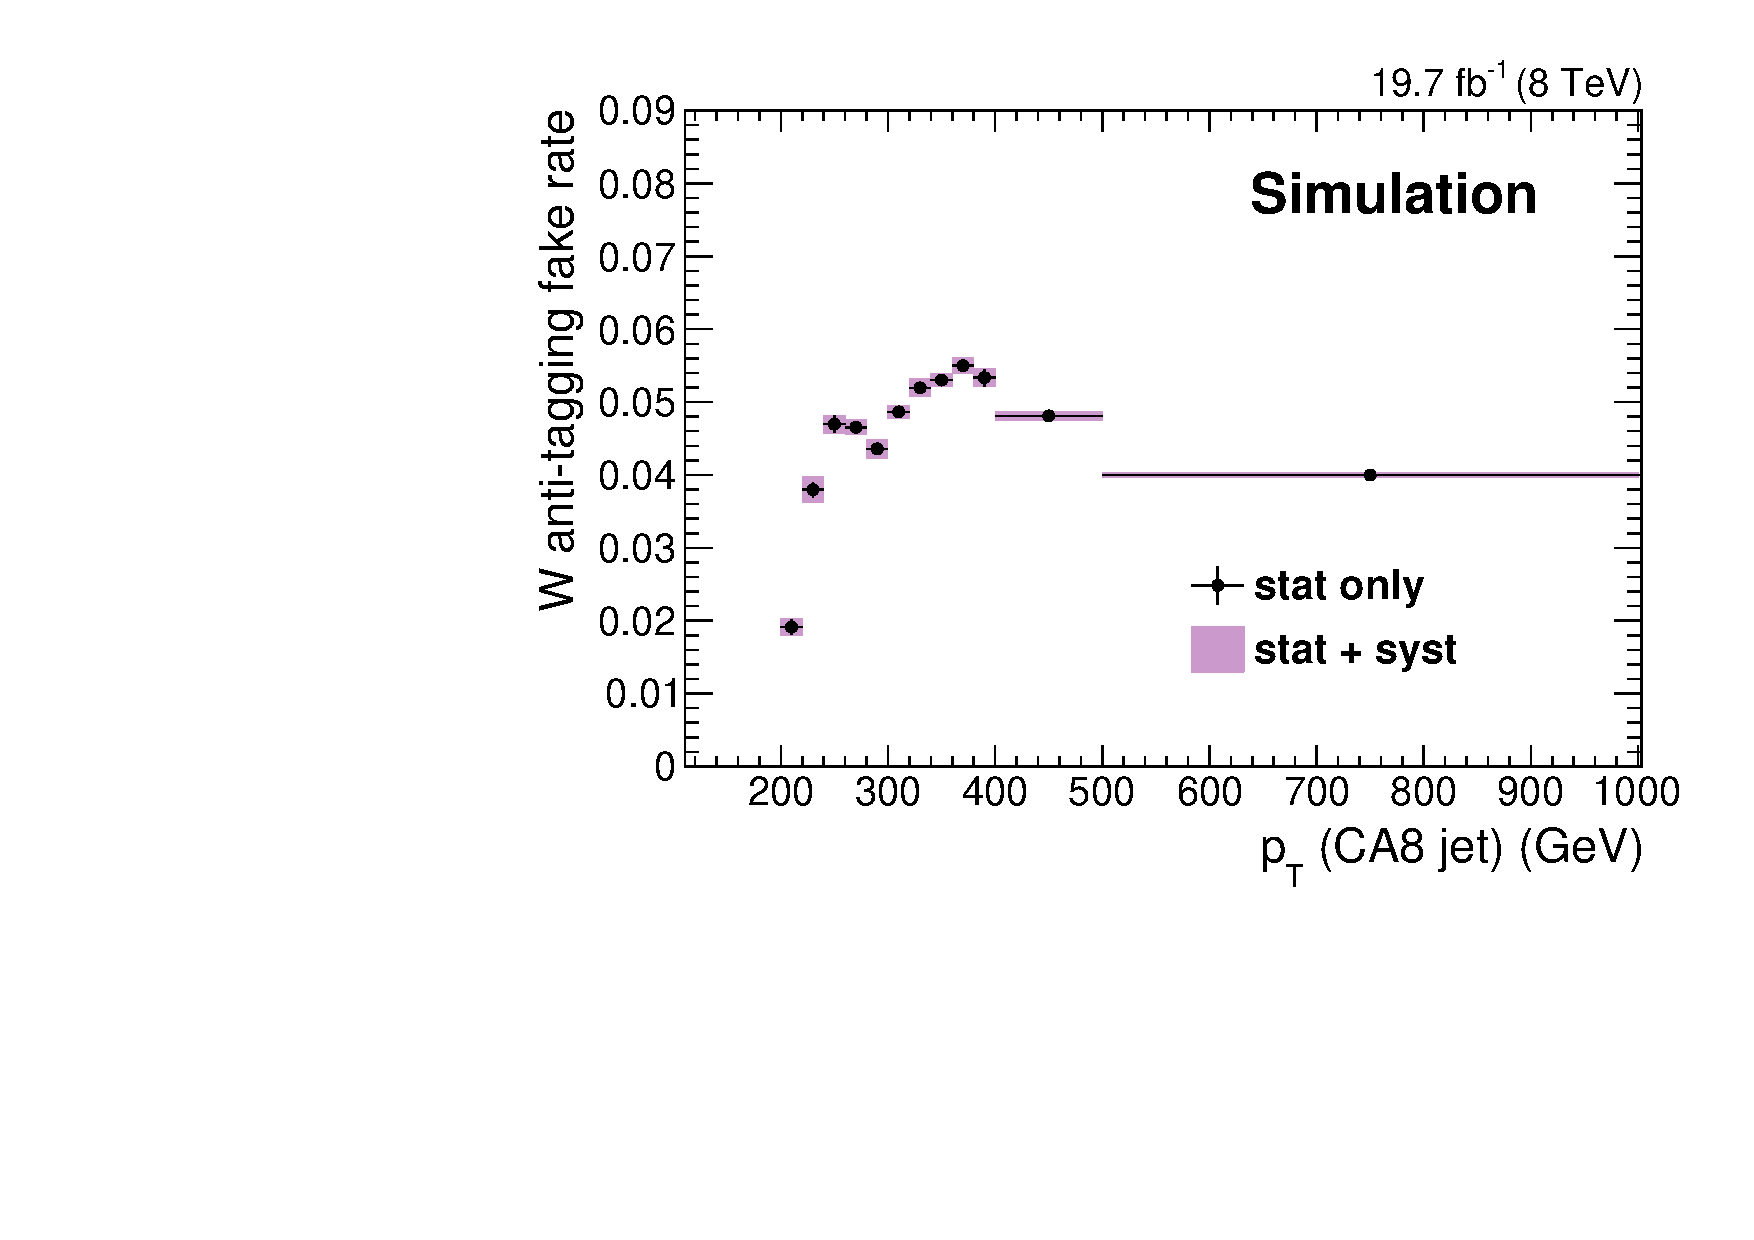
\includegraphics[width=0.6\textwidth]{figures/razor_wtag/Eff_MC_ratio_pt_antitagged_all_MC_Thesis}

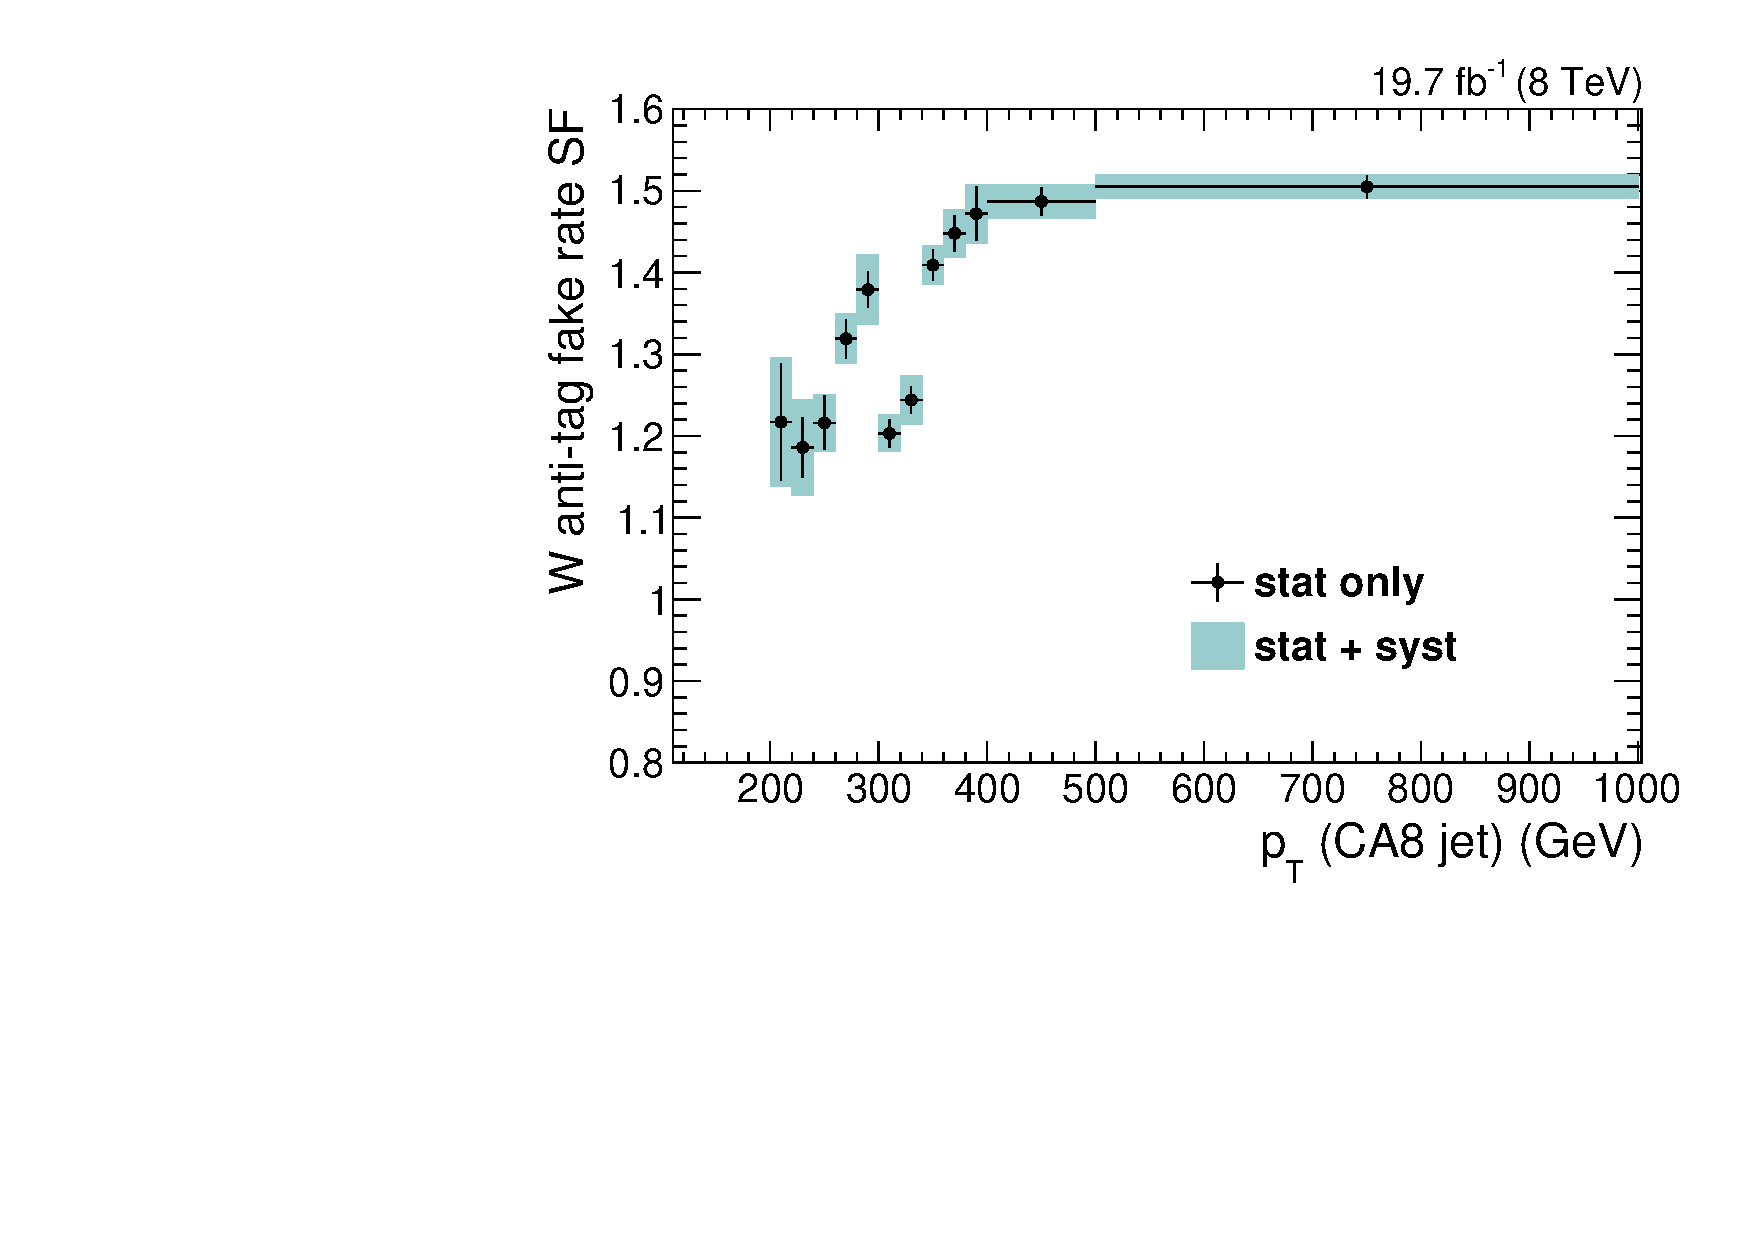
\includegraphics[width=0.6\textwidth]{figures/razor_wtag/SF_Wantitagged_Thesis}
\caption{[top] Misidentification probability according to $\W$ anti-tagging for a CA8 jet versus jet
\pt obtained from a multijet-enriched control region in data as described in the text. The shown
uncertainties are statistical only.
[middle] $\W$ boson anti-tag fake rate according to simulation. The uncertainty band includes
statistical and systematic uncertainties. 
[bottom] Scale factor for $\W$ anti-tag fake rate versus CA8 jet \pt obtained from a
multijet-enriched control region as described in the text. The uncertainty band includes
statistical and systematic uncertainties.
\label{fig:boost_wantitag}}
\end{figure}


% TODO explain the wiggle

%%%%%%%%%%%%%%%%%%%%%%%%%%%%%%%%%%%%%%%%%%%%%%%%%%%%%%%%%%%%%%%%%%%%%%%%%%%%%%%%%%%%%%%%%%%%%%%%%%%%



% 
% As we can see from these figures, there is a drop in the scale factor around a \pt of 300\GeV. 
% This is a result of a residual mismodeling of the trigger efficiency, as is explained in more detail
% in appendix~\ref{app:wiggle}. 
% Given that we understand the origin of this wiggle, we decide to keep the binning quite fine in that
% region, so that we can correct for the effect. 

\begin{table}[htbp]
\centering
\caption{Summary of scale factors and their total uncertainty. \label{tab:SF_summary}}
\vspace{1ex}
\begin{tabular}{c c c c}
\toprule
CA8 jet \pt (\GeV) & $SF_{\W\textrm{tag}}^\textrm{fake}$ & $SF_{\W \textrm{masstag}}^\textrm{fake}$
& $SF_{\W\textrm{antitag}}^\textrm{fake}$ \\
\midrule
$[200 - 220[$ & $1.04 \pm 0.07$ & $1.14 \pm 0.06$ & $1.22 \pm 0.08$ \\
$[220 - 240[$ & $1.01 \pm 0.04$ & $1.12 \pm 0.04$ & $1.19 \pm 0.06$ \\
$[240 - 260[$ & $1.16 \pm 0.04$ & $1.19 \pm 0.03$ & $1.22 \pm 0.04$ \\
$[260 - 280[$ & $1.16 \pm 0.03$ & $1.25 \pm 0.03$ & $1.32 \pm 0.04$ \\
$[280 - 300[$ & $1.15 \pm 0.03$ & $1.27 \pm 0.03$ & $1.38 \pm 0.05$ \\
$[300 - 320[$ & $1.03 \pm 0.02$ & $1.13 \pm 0.02$ & $1.20 \pm 0.03$ \\
$[320 - 340[$ & $1.14 \pm 0.02$ & $1.20 \pm 0.03$ & $1.24 \pm 0.03$ \\
$[340 - 360[$ & $1.17 \pm 0.02$ & $1.30 \pm 0.02$ & $1.41 \pm 0.03$ \\
$[360 - 380[$ & $1.18 \pm 0.03$ & $1.33 \pm 0.02$ & $1.45 \pm 0.03$ \\
$[380 - 400[$ & $1.18 \pm 0.03$ & $1.34 \pm 0.03$ & $1.47 \pm 0.04$ \\
$[400 - 500[$ & $1.15 \pm 0.02$ & $1.34 \pm 0.02$ & $1.49 \pm 0.03$ \\
$[500 - ...]$ & $1.18 \pm 0.02$ & $1.37 \pm 0.02$ & $1.51 \pm 0.02$ \\
\bottomrule
\end{tabular}
\end{table}





% explain n-subjettiness and jet pruning
% quote some plots and numbers from the JME PAS. 

\section{Signal region selection \label{sec:boost_signal_selection}}

%%%%%%%%%%%%%%%%%%%%%%
% Signal selection   %
%%%%%%%%%%%%%%%%%%%%%%

The signal region selection aims for a good discrimination between possible signals and the SM
backgrounds. As mentioned before, the signals we target with this search have $\cPqb$ tagged jets
and boosted $\W$ bosons in the final state. Therefore, we require, on top of the baseline
selection, the presence of at least one CSV medium $\cPqb$ tagged jet, and at least one $\W$ boson
tagged jet. AK5 jets are used for $\cPqb$ tagging, whereas for $\W$ tagging we use the CA8 jets, as
explained in Section~\ref{sec:boost_wtag}. 
Additionally, we only consider fully-hadronic events and thus select only those events without
loose electrons or muons, and no isolated tracks. 
These selection criteria already reduce the background substantially, but the achieved signal
separation is not yet sufficient. We need an additional handle on the QCD multijet production,
which is the dominant background at this stage. 

Missing transverse energy, \ETm, in multijet events is largely due to jet mismeasurements,
rather than the escape of weakly interacting particles, such as neutrinos or the neutralinos in
signal events. The \ETm vector will, therefore, often be aligned with one of the jets. 
Based on this we can expect that $\Delta\phi_{min}$, the minimum of the angles between \VEtmiss and
the transverse momentum of the leading three jets, will be a good discriminant between multijet
events and events with real \ETm.
\begin{equation}
 \Delta\phi_{min} = \min_{i=1,2,3}{\Delta\phi(\VEtmiss, \ptvec^{\,i})},
\end{equation}
where $i$ runs over the three leading AK5 jets. We require $\Delta\phi_{min} > 0.5$ to suppress
multijet events. The $\Delta\phi_{min}$ distribution, obtained from simulation, before applying this
selection is shown in
Fig.~\ref{fig:boost_signal_mindeltaphi}. The multijet events are clearly gathered in the first few
bins.

\begin{figure}[htbp]
 \centering
 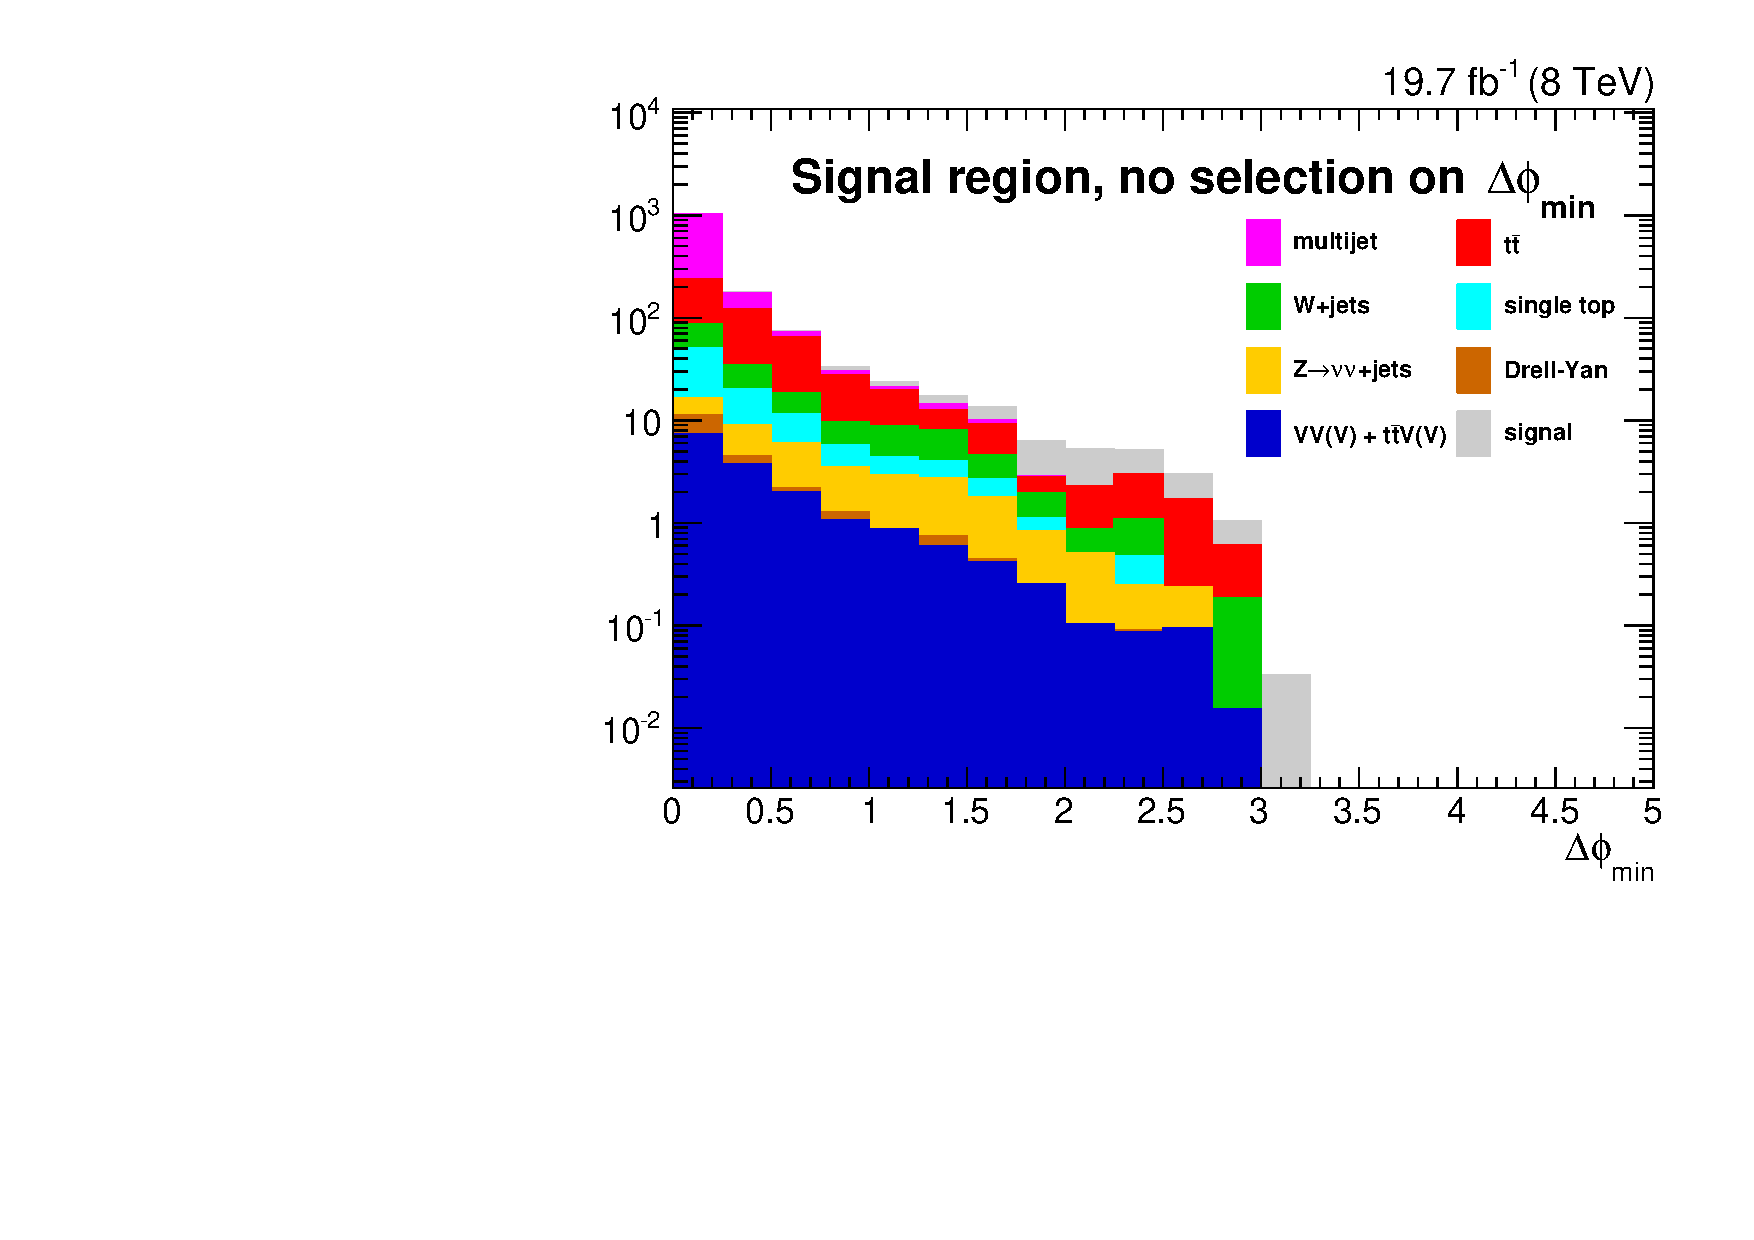
\includegraphics[width=0.7\textwidth]
 {figures/razor_selection/plots/DataMC_minDeltaPhi_g1Mbg1W0Ll_rebin_nodata}
\caption{Simulated $\Delta\phi_{min}$ distribution with all signal region requirements applied
except $\Delta\phi_{min} > 0.5$. QCD multijet events are clearly gathered in the first few bins.
\label{fig:boost_signal_mindeltaphi}}
\end{figure}

A summary of the signal selection is presented in Table~\ref{tab:boost_selection_summary}.
Figure~\ref{fig:boost_signal_dataMC} shows the simulated distributions in the signal region for the
$\mr$ and $\rsq$ variables. The number of events in simulation and data, and the background
composition in percent, are reported in Table~\ref{tab:cutflow} and
Table~\ref{tab:BG_comp_percent}, respectively. 
The signal region is $t\bar{t}$ dominated, with additional contributions from $\W(\rightarrow
\ell\nu)+$jets and multijet processes.
The \pt distribution of the highest \pt tagged $\W$ boson jet in the event is shown in
Fig.~\ref{fig:boost_signal_Wpt_met}, alongside the \ETm distribution.  

\begin{figure}[htbp]
\centering
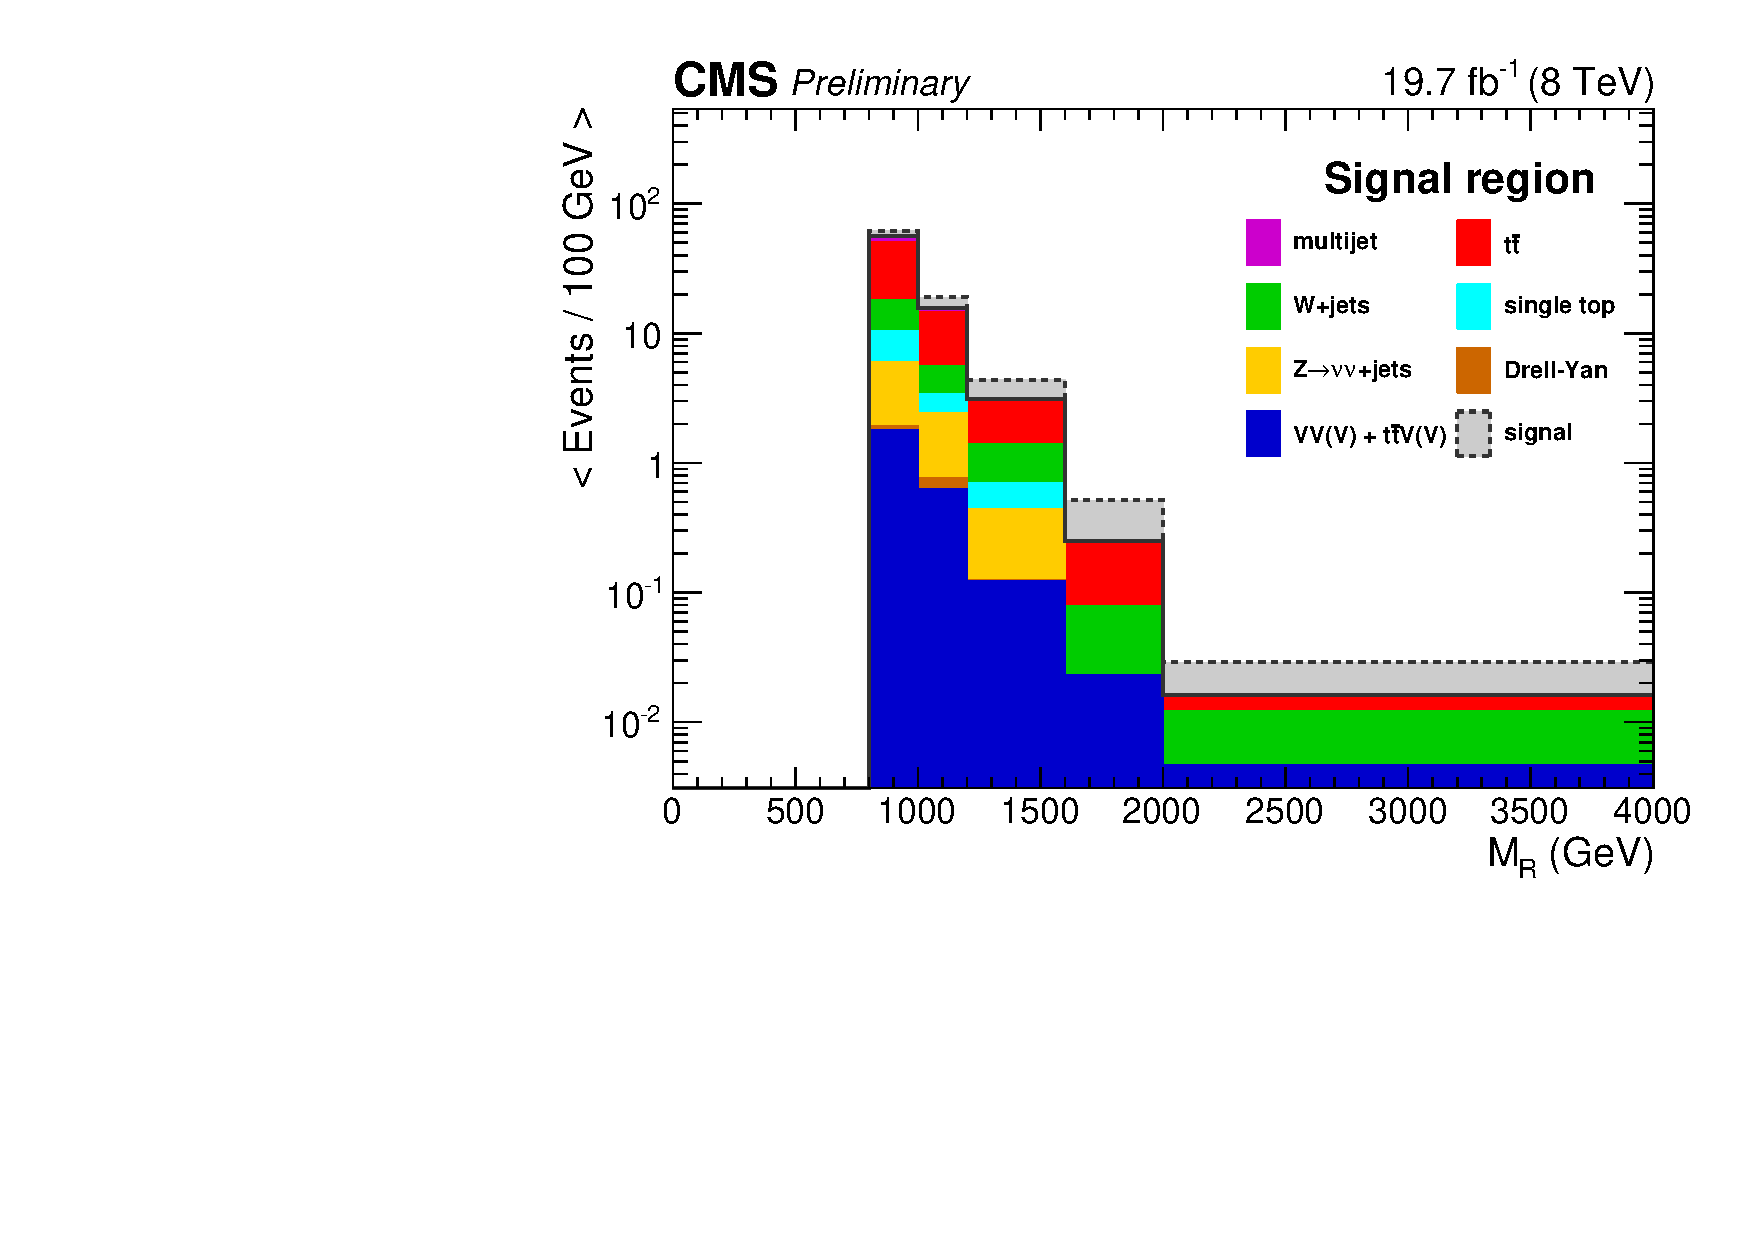
\includegraphics[width=0.48\textwidth]
{figures/razor_selection/DataMC_MR_g1Mbg1W0Ll_mdPhig0p5_width_nodata}
~
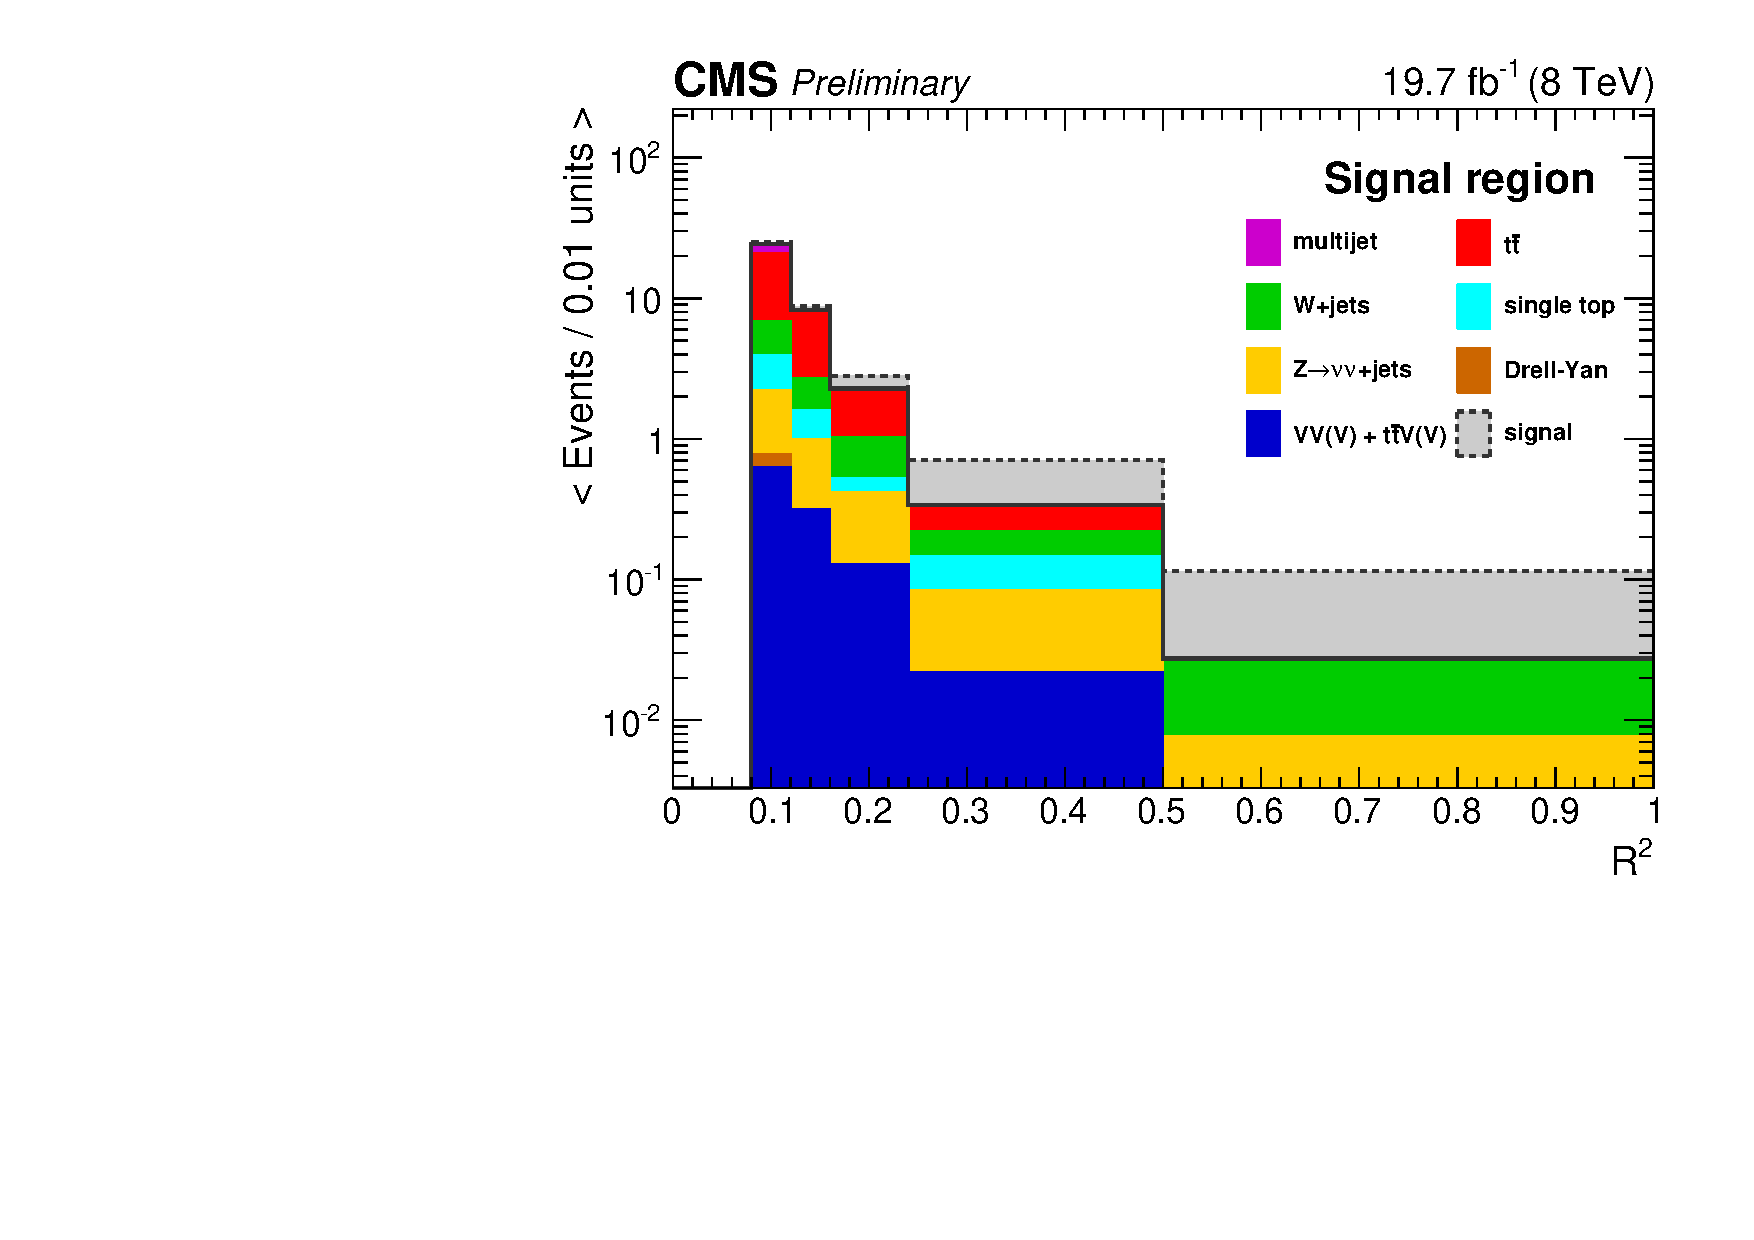
\includegraphics[width=0.48\textwidth]
{figures/razor_selection/DataMC_R2_g1Mbg1W0Ll_mdPhig0p5_width_nodata}
\caption{Simulated $\mr$ (left) and $\rsq$ (right) distributions in the signal region. An example
signal point, corresponding to the T1ttcc mass point with $m_{\tilde{g}}
\,{=}\, 1\TeV$, $m_{\stopone} \,{=}\, 325\GeV$ and $m_{\lsp} \,{=}\, 300\GeV$, is
stacked on top of the background processes. The bin entries are normalized proportional to the bin
width.  
\label{fig:boost_signal_dataMC}}
\end{figure}

\begin{figure}[htbp]
\centering
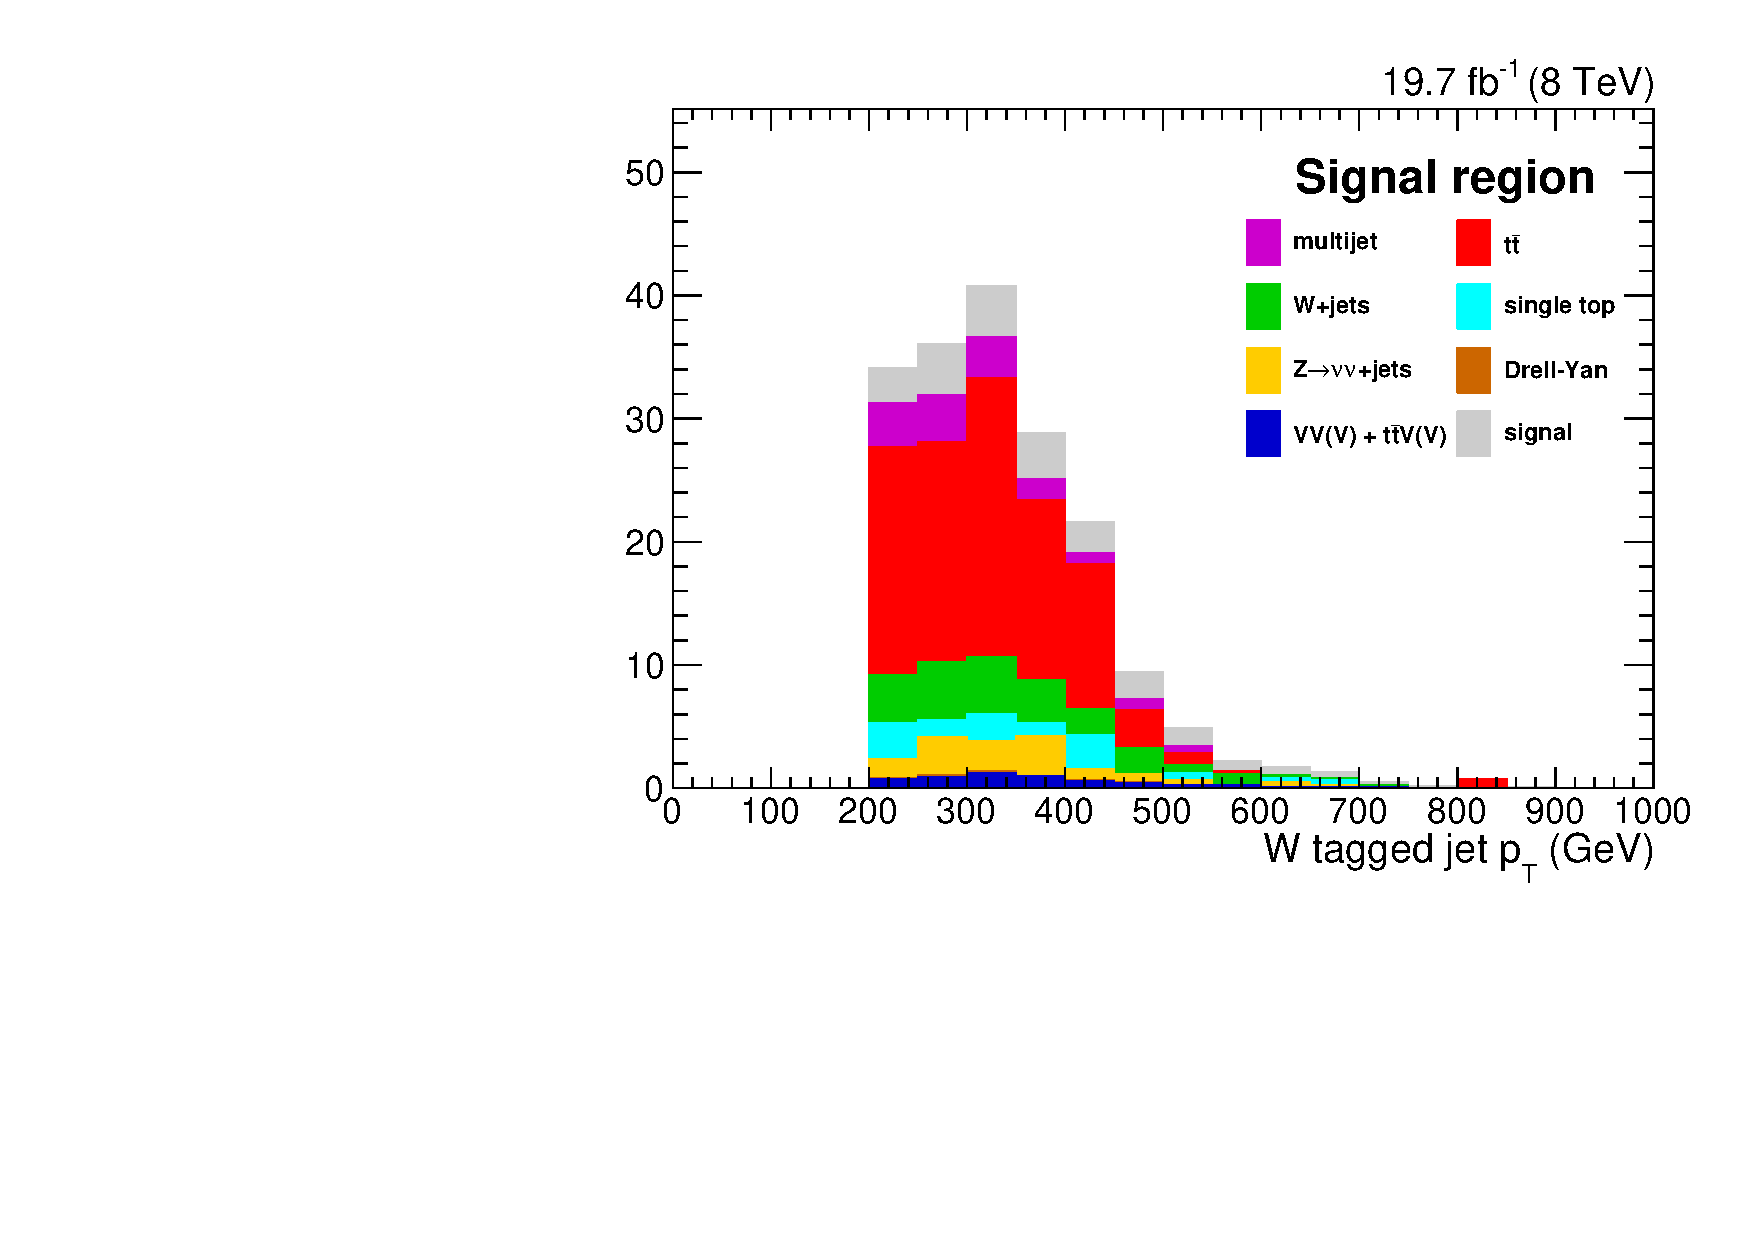
\includegraphics[width=0.48\textwidth]
{figures/razor_selection/plots/DataMC_Wpt_g1Mbg1W0Ll_mdPhig0p5_nodata}
~
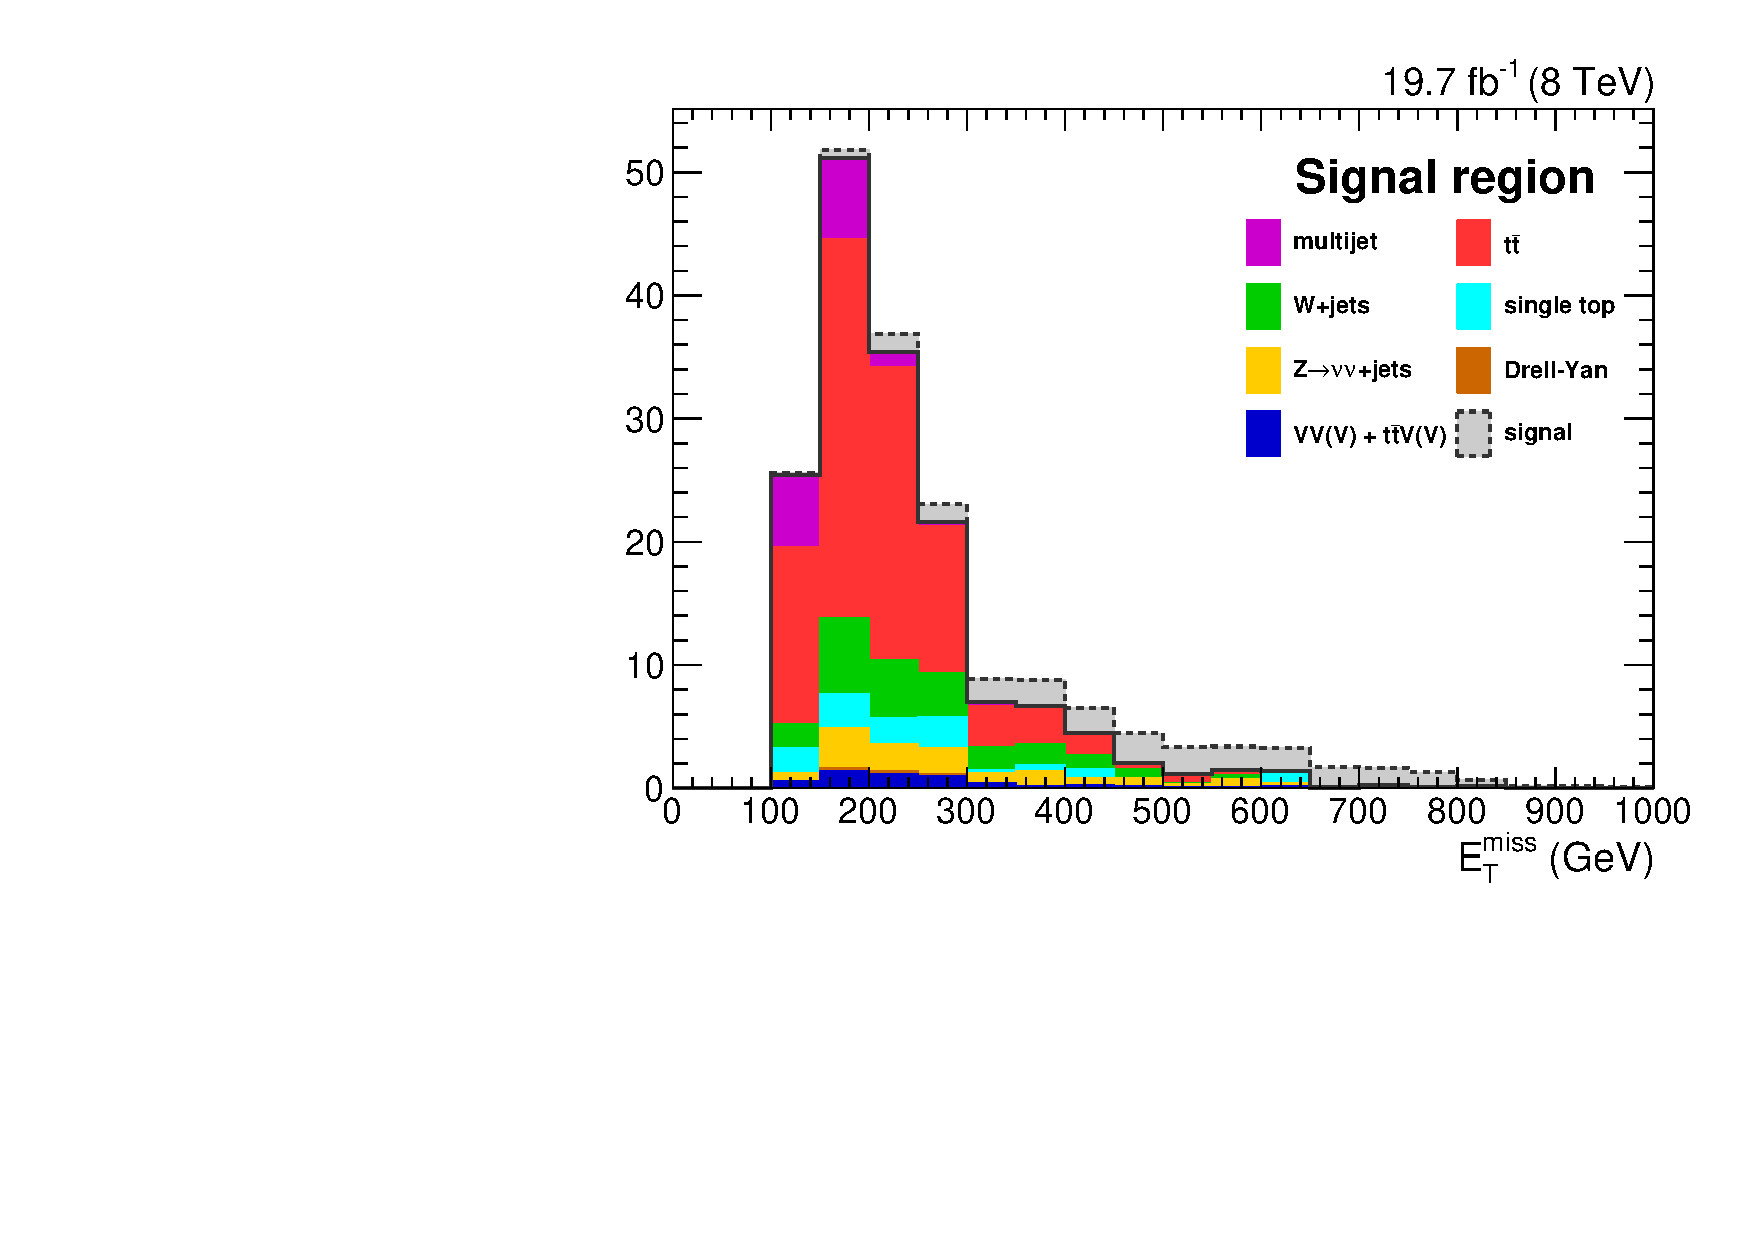
\includegraphics[width=0.48\textwidth]
{figures/razor_selection/plots/DataMC_met_g1Mbg1W0Ll_mdPhig0p5_nodata}
\caption{Simulated $\W$ tagged jet $\pt$ (left) and $\ETm$ (right) distributions in the signal
region. An example signal point, corresponding to the T1ttcc mass point with $m_{\tilde{g}}
\,{=}\, 1\TeV$, $m_{\stopone} \,{=}\, 325\GeV$ and $m_{\lsp} \,{=}\, 300\GeV$, is
stacked on top of the background processes. 
\label{fig:boost_signal_Wpt_met}}
\end{figure}



% In figures~\ref{fig:DataMC_SignalRegion_MR_R2_mdphig0p5} and \ref{fig:DataMC_SignalRegion_mdphig0p5}
% we show a Data/MC comparison for various quantities for the signal region with $\Delta\phi_{min} >
% 0.5$. 
% Please note that these plots are for illustration purposes only. 
% We will predict the background using data control regions and only use the simulation for
% translation factors between those control regions and the signal region (see further). We stress in
% particular that the QCD multijet MC is underpredicting what we see in data.
% 
% \begin{figure}[p]
%  \includegraphics[width=0.49\textwidth]{figures/DataMC/DataMC_njets_g1Mbg1W0Ll_mdPhig0p5}
%  \includegraphics[width=0.49\textwidth]{figures/DataMC/DataMC_nbjets_g1Mbg1W0Ll_mdPhig0p5}
% 
%  \includegraphics[width=0.49\textwidth]{figures/DataMC/DataMC_met_g1Mbg1W0Ll_mdPhig0p5}
%  \includegraphics[width=0.49\textwidth]{figures/DataMC/DataMC_jet1pt_g1Mbg1W0Ll_mdPhig0p5}
% 
%  \includegraphics[width=0.49\textwidth]{figures/DataMC/DataMC_jet2pt_g1Mbg1W0Ll_mdPhig0p5}
%  \includegraphics[width=0.49\textwidth]{figures/DataMC/DataMC_jet3pt_g1Mbg1W0Ll_mdPhig0p5}
% \caption{For illustration only: Data/MC comparison plot of various event quantities in the signal
% region requiring $\Delta\phi_{min} > 0.5$: 
% [top] jet multiplicity (left) and b-tagged jet multiplicity (right);
% [middle] missing transverse energy (left) and \pt of the highest \pt jet (right);
% [bottom] \pt of the second (left) and third (right) highest \pt jet. 
% \label{fig:DataMC_SignalRegion_mdphig0p5}}
% \end{figure}
% 
% \begin{figure}[htbp]
%  \includegraphics[width=0.49\textwidth]{figures/DataMC/DataMC_Wpt_g1Mbg1W0Ll_mdPhig0p5}
%  \includegraphics[width=0.49\textwidth]{figures/Shapes/comparison_Wpt}
% \caption{For illustration only: [left] Data/MC comparison plot of $\pt(W)$ in the signal region
% requiring $\Delta\phi_{min} > 0.5$.
% [right] Comparison of the $\pt(W)$ distribution for signal and total background. Both distributions
% are normalized to unit area.
% \label{fig:Wpt_SignalRegion}}
% \end{figure}
% 


\section{Control region selection \label{sec:boost_control_selection}}

\section{Statistical modelling \label{sec:boost_likelihood}}

%%%%%%%%%%%%%%%%%%%%%
% Likelihood stuff
%%%%%%%%%%%%%%%%%%%%%

% TODO \textcolor{red}{This section has been copied directly from the paper draft. It will be
% expanded upon in a next version.}



The statistical analysis of the observations,  $\{ N^S_i \}$, in the signal region is based on a
likelihood function, $L(\sigma)$, given by
\begin{align}
  L(\sigma) & \equiv  \int   \left[ \prod_{i=1}^M p(N^S_i | \sigma, {\cal L}, \theta_i)  \right] 
\pi(\theta) \, \pi({\cal L}) \, d\theta \, d{\cal L},
\label{eq:marginal}
\end{align}
where $\sigma$ is the total signal cross section, $M = 25$ is the number of bins, $N^S_i$ the
observed count in bin $i$, and the bin-by-bin parameters  $\epsilon$,  $b^S_{QCD}, b^S_{TTJ},
b^S_{\W\ell\nu}$, and $b^S_{oth}$ are  denoted collectively by $\theta$. 
The function $\pi({\cal L})$ is the integrated luminosity prior and $\pi(\theta)$ is an evidence
based prior constructed from observations in the control regions and the four global scale factors
$\kappa^{A/B}_{process}$ determined by simulated data. 
The parameter $\epsilon$ represents the $M$ signal efficiencies (including acceptance) for a given
signal model. Figure~\ref{fig:boost_flowchart} shows which control regions provide constraints on
the background parameters, $b^S_{process}$.
The likelihood per bin is taken to be
\begin{equation}
 p(N^S | \sigma, {\cal L}, \theta) = \textrm{Poisson}(N^S,  \epsilon \sigma {\cal L} + b^S_{QCD} +
b^S_{TTJ} + b^S_{\W\ell\nu} +  b^{S}_{oth}) .
\end{equation}

\begin{figure}[p]
  \centering
  \includegraphics[width=\textwidth]{figures/razor_strategy/BoostFlowChart_noZ}
  \caption{Definition of, and relationship between, the signal ($S$) and control ($Q,T,W$) regions
and their relationship to the bin-by-bin background parameters
$b^{\textrm{region}}_{\textrm{process}}$ for a given region and background process, as well as the
four global scale factors $\kappa^{A/B}_{\textrm{process}} = \sum_i b^A_{\textrm{process}, MC, i} /
\sum_i b^B_{\textrm{process}, MC, i}$, where the sum is over all 25 (\mr,\rsq) bins of the simulated
data. 
The total expected background, per bin, is the sum of the terms shown for each region. Furthermore,
associated with each bin of each region is an observed count $N^{\textrm{region}}$, a simulated
count $N^{\textrm{region}}_{\textrm{process}, MC}$, and a count $N^{\textrm{region}}_{oth, MC}$
equal to the sum of the smaller backgrounds, with associated parameter $b^{\textrm{region}}_{oth}$.
  \label{fig:boost_flowchart}}
\end{figure}

The integral in Eq.~(\ref{eq:marginal}) is approximated by Monte Carlo integration by sampling
 the priors $\pi({\cal L})$, and  $\pi(\theta)$. 
The priors for the expected integrated luminosity, ${\cal L}$, signal efficiencies, $\epsilon$, and 
simulated background counts, $b^{region}_{process, MC}$, are modelled with gamma densities,
\begin{align}
\textrm{gamma}(x, \gamma, \beta) &= \beta^{-1}(x/\beta)^{\gamma-1} \exp(-x / \beta) /
\Gamma(\gamma),
\label{eq:gamma}
\end{align}
in which the mode is set to $c$ and the variance to $\delta c^2$, 
where $c \pm \delta c$ denotes either the measured integrated luminosity, or for a given bin of
a given region and process, the simulated signal efficiency, or the simulated background count. This
yields the gamma density parameters,
\begin{align}
   \gamma &= [(k + 2) + \sqrt{(k+2)^2 - 4}]/2,\\
   \beta &= [\sqrt{c^2 + 4\delta c^2} - c]/2,
\end{align}
where $k = (c / \delta c)^2$.
For empty bins, we set $\gamma = 1$ and the bin value is constrained to zero by setting the $\beta$
parameter to $10^{-4}$.
 
For the signal efficiencies and backgrounds, the prior is modelled hierarchically,
\begin{align}
  \pi(\theta) = \int \pi(\theta | c ) \, \pi(c | \phi ) \pi(\phi) \, dc d\phi,
  \label{eq:prior}
\end{align}
where $c$ is a simulated count or efficiency in an $(\mr,  \rsq)$ bin and $\phi$ represents
parameters that characterize the independent sources of systematic uncertainty, described in
Section~\ref{sec:boost_systematics}. 
The integral in Eq.~(\ref{eq:prior}) is evaluated as follows: $\phi$ values are sampled from
$\pi(\phi)$, then $c$ values from $\pi(c | \phi)$, then $\theta$ values from $\pi(\theta | c)$. 
The sampling from $\pi(\phi)$ and $\pi(\theta|c)$ is straightforward because the functional forms
are known. However, the sampling of $c$ requires running the analysis multiple times.
The independent sources of systematic uncertainty are sampled simultaneously, which produces an
ensemble of sets of $(\mr, \rsq)$ histograms for the simulated backgrounds and efficiencies, for all
signals under consideration, that automatically incorporate all statistical dependencies
without the need to model them explicitly.  The ensemble of histograms is the output of the
procedure described in Section~\ref{sec:boost_systematics}. Thereafter, the sampling proceeds as
follows:
\begin{enumerate}
\item sample the integrated luminosity parameter;
\item sample the efficiency parameters, $\epsilon$, for every signal model;
\item sample the parameters $b^{region}_{process, MC}$ of the simulated background densities and sum
their values over the $M$ bins;
\item compute the $\kappa$ parameters from the appropriate background sums (for example,
$\kappa^{Q/S}_{QCD} =  \sum_i  b^Q_{QCD, MC, i} / \sum b^S_{QCD, MC, i}$);
\item scale each $\kappa$ value by a random Gaussian variate of unit mean and standard deviation
of 0.33 to account for additional uncertainty in $\kappa$ due to deficiencies in the simulated
 data, and 
\item sample the background parameters $b^S_{QCD}$, $b^S_{TTJ}$, and $b^S_{\W\ell\nu}$, from the 
Poisson models  of the control regions; for example, for region $Q$, we map  $\textrm{Poisson}(N^Q
, \kappa^{Q / S} b^S_{QCD} + b^Q_{oth})$ to a posterior density in $b^S_{QCD}$ using a flat prior
and sample $b^S_{QCD}$ from that density.
\end{enumerate}

In the absence of  a signal, we determine limits on the total signal cross section using the CLs
criterion~\cite{LHCCLs} and the test statistic $t_\sigma = 2 \ln [ L(\hat{\sigma}) /  L(\sigma)]$
when $0 \leq\hat{\sigma} \leq \sigma$, and $t_\sigma = 0$ when $\hat{\sigma} > \sigma$. 
Large values of $t_\sigma$ indicate incompatibility between the best fit hypothesis $\sigma^\prime 
= \hat{\sigma}$ and the entertained hypothesis $\sigma^\prime  = \sigma$. 
We calculate  the p-values $p_0 = \textrm{Prob}(t_\sigma > t_{\sigma, obs} | \sigma^\prime = 0)$ 
and $p_\sigma = \textrm{Prob}(t_\sigma > t_{\sigma, obs} | \sigma^\prime=\sigma)$, needed to
calculate $\textrm{CLs}(\sigma) = p_\sigma / p_0$,  by simulation. 
The quantity $t_{\sigma, obs}$ denotes the observed values of the test statistic, one for each
hypothesis $\sigma^\prime=\sigma$.




% \section{Likelihood \label{sec:likelihood}}
% 
% \subsection{Introduction \label{sec:intro}}
% The probability model for this analysis consists of a multi-Poisson 
% likelihood for the signal
% region and a prior that models the uncertainties in 
% the integrated luminosity, ${\cal L}$, the signal efficiencies,
% $\epsilon$ (which includes the
% acceptance), and the backgrounds. The total 
% cross section of the signal,
% $\sigma$, is the parameter of interest. The structure of the model is shown in
% Fig.~\ref{fig:BoostWorkflow}. 
% There is one signal region, $S$, in which the search is conducted and three control regions, $Q$,
% $T$, and  $W$, which are used to constrain the expected QCD, top, and W backgrounds,
% $b^S_{QCD}$, $b^S_{TTJ}$, and $b^S_{W\ell\nu}$, respectively,
%  in the signal region~\footnote{In the symbol
%    $X^{region}_{component}$, the superscript labels the region ---
%    either 
% the signal region, $S$,
%  or a control 
% region, $Q$, $T$, or $W$ --- while the subscript labels the background
% component 
% within the region. Since this analysis uses both real
%  and simulated data, we distinguish symbols pertaining to simulated
%  data  by 
% appending the subscript $MC$.}.
% Simulated data in each of the four
% regions are used to constrain the
% small expected 
% background counts $b_{oth}^j$, $j = S, Q, T, W$ and
% four global scale factors 
% $\kappa^{Q/S}_{QCD}$,  $\kappa^{T/S}_{TTJ}$, $\kappa^{Q/T}_{QCD}$, and
% $\kappa^{W/S}_{QW\ell\nu}$, defined as the ratio of the expected background
% component in a control region to that in the signal (or another control) region.
% For example, the factor $\kappa^{Q/S}_{QCD}$ is the ratio of the
% expected 
% QCD background
% in the $Q$ region to that in the $S$ region. The scale factors can
% be estimated by the inverse of the MC ratios defined in
% Eqs.~(\ref{eq:E1})--(\ref{eq:E4})~\footnote{These
% ratios, which are ratios of
% MC counts, 
% $N^{region}_{component, MC}$ are not used in the model; rather 
% the model is written in terms of the $\kappa$ parameters.}. As noted
% above, global scale factors are used because 
% the statistical precision of some of the
% simulated data precludes the use bin-by-bin scale
% factors. Deficiencies in MC modeling are accounted for by assigning 
% appropriate uncertainties to the global factors, as described in 
% Section~\ref{sec:systematics}.
% 
% 
% 
% Below, we give
% brief 
% descriptions of each of the four 
% regions and provide some details of the statistical modeling. 
% In subscripts, the top contribution is
% written
% as $TTJ$, rather than $TTJ+T$, where it is to be understood that the
% top
% contribution includes single top.
% 
% \subsection{Signal Region}
% 
% Tthe background in the signal region is divided into four components,
% \begin{enumerate}
% 	\item QCD
% 	\item TTJets + T
% 	\item WJets
% 	\item Other (VV, VVV, TTX, Zll, Wbb, Z$\nu\nu$),
% \end{enumerate}
% with expected (i.e., mean) count per bin $b^S_{QCD}$, $b^S_{TTJ}$, $b^S_{Wl\nu}$, and
%  $b^S_{oth}$, respectively. 
% The quantities pertaining to the signal region are:
% \begin{align}
%  \textrm{\bf components}\nonumber\\
%  \textrm{QCD, TTJets+T, WJets, Other}\nonumber\\
%  %
%   \textrm{\bf observed count} 	& \quad\textrm{\bf expected count} \nonumber\\
%   	N^S 
% 	&\quad \sigma \epsilon {\cal L} + b^S_{QCD} + b^S_{TTJ} +
%         b^S_{Wl\nu} +  b^{S}_{oth, MC} 
% 	\nonumber\\
% %
% 	\textrm{\bf MC counts}	& \quad\textrm{\bf expected counts}	
% 	\nonumber\\
% 	N^{S}_{QCD, MC} 		& \quad b^{S}_{QCD, MC}
% 		\nonumber\\ 
% 	N^{S}_{TTJ, MC} 		& \quad b^{S}_{TTJ, MC}  
% 			\nonumber\\ 
% 	N^{S}_{W\ell\nu, MC} 	& \quad b^{S}_{W\ell\nu, MC} 
% 		\nonumber\\ 		
% 	N^{S}_{oth, MC} 		& \quad b^{S}_{oth, MC}	
% \end{align}
% The likelihood per bin is given by, 
% \begin{align}
%   p(N^S| \sigma, \theta) = \textrm{Poisson}(N^S,  \sigma \epsilon {\cal L} + b^S_{QCD} + b^S_{TTJ}
%+ b^S_{Wl\nu} +  b^{S}_{oth, MC}),
%   \label{eq:likelihood}
% \end{align}
% where $\theta$ denotes the nuisance
% parameters $\epsilon$, ${\cal L}$, $b^S_{QCD}, b^S_{TTJ}$,
% $b^S_{Wl\nu}$, and $b^S_{oth, MC}$. 
% The integrated
%  luminosity, the signal efficiency, and the
% simulated background, are modeled 
% with gamma densities, Eq.~(\ref{eq:gamma}).
% 
% 
% \subsection{Control Regions}
% The data counts in a control region are modeled with Poisson distributions, 
% while the
% simulated backgrounds are modeled 
% with gamma densities, Eq.~(\ref{eq:gamma}).
%  
% \paragraph*{Q Region}
% For each bin, this region constrains the parameter $b^S_{QCD}$, given
% $N^Q$, $b^Q_{oth, MC}$ and $\kappa^{Q/S}_{QCD}$.
%  \begin{align}
%  \textrm{\bf components}\nonumber\\
%  \textrm{QCD, Other}\nonumber\\
%  %
%   \textrm{\bf observed count} 	& \quad\textrm{\bf expected count}
%   \nonumber\\
%  	N^Q 					& \quad\kappa^{Q/S}_{QCD} \, b^S_{QCD}  + 
%b^{Q}_{oth, MC} 
% 	\nonumber\\ 
% %
% 	\textrm{\bf MC counts}	& \quad\textrm{\bf expected counts}
% 	\nonumber\\
% 	N^{Q}_{QCD, MC} 		& \quad b^Q_{QCD,MC} = \kappa^{Q/S}_{QCD} \, b^{S}_{QCD, MC}
% 	\nonumber\\ 	
% 	N^{Q}_{oth, MC} 		&\quad b^{Q}_{oth, MC}	
% \end{align}
% 
% \paragraph*{T Region}
% For each bin, this region constrains the parameter $b^S_{TTJ}$, given
% $N^T$, $b^T_{oth, MC}$, $b^S_{QCD}$,  $\kappa^{T/S}_{TTJ}$,
% $\kappa^{T/Q}_{QCD}$, 
% and $\kappa^{Q/S}_{QCD}$.
%  \begin{align}
%  \textrm{\bf components}\nonumber\\
%  \textrm{TTJets, QCD, Other}\nonumber\\
%  %
%   \textrm{\bf observed count} 	& \quad\textrm{\bf expected count}
%   \nonumber\\
%  	N^T 					& \quad\kappa^{T/S}_{TTJ} \, b^S_{TTJ}  
% 	+ \kappa^{T/Q}_{QCD} \, \kappa^{Q/S}_{QCD} \, b^S_{QCD}  
% 	+  b^{T}_{oth, MC} 
% 	\nonumber\\ 
% %
% 	\textrm{\bf MC counts}	& \quad\textrm{\bf expected counts}
% 	\nonumber\\
% 	N^{T}_{TTJ, MC} 		& \quad b^T_{TTJ, MC} = \kappa^{T/S}_{TTJ} \, b^{S}_{TTJ,
%MC}
% 	\nonumber\\ 
% 	N^{T}_{QCD, MC} 		& \quad b^T_{QCD, MC} = \kappa^{T/Q}_{QCD} \,
%\kappa^{Q/S}_{QCD} \, b^{S}_{QCD,MC}  
% 	\nonumber\\ 	
% 	N^{T}_{oth, MC} 		&\quad b^{T}_{oth, MC}
% \end{align}
% 
% \paragraph*{W Region}
% For each bin, this region constrains the parameter $b^S_{W\ell\nu}$, given
% $N^W$, $b^W_{oth, MC}$ and $\kappa^{W/S}_{W\ell\nu}$.
%  \begin{align}
%  \textrm{\bf components}\nonumber\\
%  \textrm{WJets, Other}\nonumber\\
%  %
%   \textrm{\bf observed count} 	& \quad\textrm{\bf expected count}
%   \nonumber\\
%  	N^W					& \quad\kappa^{W/S}_{W\ell\nu} \, b^S_{W\ell\nu}    
% 	+  b^{W}_{oth, MC} 
% 	 \nonumber\\ 
% %
% 	\textrm{\bf MC counts}	& \quad\textrm{\bf expected counts}\nonumber\\
% 	N^{W}_{W\ell\nu, MC} 	& \quad b^W_{W\ell\nu, MC} = \kappa^{W/S}_{W\ell\nu} \,
%b^{S}_{W\ell\nu, MC}
% 	 \nonumber\\ 
% 	N^{W}_{oth, MC} 		&\quad b^{W}_{oth, MC}
% \end{align}
% 
% \subsection{Priors
% \label{sec:priors}}
% The integrated luminosity, the signal efficiencies, and 
% the simulated background counts --- where $c \pm \delta c$ denotes the
% value in an $(\mathrm{M_R}, \mathrm{R^2})$ bin
% and its
% uncertainty --- are modeled with gamma priors of the form, 
% \begin{align}
% \beta^{-1}(x/\beta)^{\gamma-1} \exp(-x / \beta) / \Gamma(\gamma),
% \label{eq:gamma}
% \end{align}
% in which the mode is set to $c$
% and the variance to $\delta c^2$, yielding 
%  \begin{align}
%  	\gamma &= [(k + 2) + \sqrt{(k+2)^2 - 4}]/2,\\
% 	\beta &= [\sqrt{c^2 + 4\delta c^2} - c]/2,
%  \end{align}
% for the gamma density parameters,
%  where $k = (c / \delta c)^2$. For empty bins, $\gamma = 1$ and the bin value is
%  constrained to zero by 
%  setting the $\beta$ parameter to $10^{-4}$.
%  
% \subsection{Final likelihood}
% Several systematic uncertainties in this analysis induce
% correlations
% across the bins of all signal and background models. A canonical example
% is the jet energy scale, which when varied 
% induces coherent shifts in the signal and background
% models. The standard way to
% handle these shifts is to model explicitly (by fitting a large number
% of empirical functions) the
% dependence of the likelihood parameters on the parameters of the underlying sources of
% uncertainty and by making assumptions about how parameters
% are correlated. 
% 
% In this analysis, we  approach the problem
% differently. 
% Uncertainties are accounted for by 
% marginalizing,
% \begin{align}
%   p(D^S| \sigma)	 & = \int   \left[\prod_{i=1}^M p(N^S_i|
%     \sigma, \theta)\right] 
% \pi(\theta) \, d\theta,
% \label{eq:marginal}
% \end{align}
%  the likelihood $p(D^S|\sigma, \theta)$ 
% with respect to an evidence based
% prior $\pi(\theta)$, where $D^S \equiv N^S_1,\cdots, N^S_K$ and $K = 25$
% is
% the number of bins. 
% The integral
% is approximated by Monte Carlo integration,
% \begin{align}
%     p(D^S| \sigma) & \approx \frac{1}{J} \sum_{j=1}^J \prod_{i=1}^K
%     p(N^S_i| \sigma, \theta_j),
% \end{align}
% using $J$ points $\theta_j$ randomly sampled from the prior
% $\pi(\theta)$. Since the
% background model closely matches the data, the points
% $\theta_j$ are well matched to the likelihood. Consequently, 
% with a few hundred 
% points,
% Monte Carlo integration
% provides a good approximation to the integral in Eq.~(\ref{eq:marginal})
% 
% In practice, the prior $\pi(\theta)$ is modeled
% hierarchically,
% \begin{align}
%   \pi(\theta) = \int \pi(\theta | c ) \, \pi(c |
%   \phi ) \pi(\phi) \, dc d\phi,
%   \label{eq:prior}
% \end{align}
% where, again, $c$ is an $(\mathrm{M_R},  \mathrm{R^2})$ bin value 
% and $\phi$ represents parameters that characterize the independent
% sources
% of systematic uncertainty. The integral in Eq.~(\ref{eq:prior}) is
% evaluated
% as follows: one samples $\phi$
% values from
% $\pi(\phi)$,
% then $c$ values from $\pi(c | \phi)$, then $\theta$ values from
% $\pi(\theta | c)$. The sampling from $\pi(\phi)$ and $\pi(\theta|c)$
% is straightforward because the functional forms are known. However, 
% the sampling of $c$ requires running the analysis multiple times.
% 
% 
% One crucial difference with respect to the standard method
% is that we 
% sample \emph{simultaneously} from the priors of the
% independent sources of uncertainty (see
% Section~\ref{sec:systematics}). 
% This procedure produces an
% ensemble of sets of $(\mathrm{M_R}, \mathrm{R^2})$ histograms for
% the simulated backgrounds and the efficiencies for all signals
% under
% consideration. Thereafter, the sampling proceeds as follows. 
% For a given set of $c \pm \delta c$ values:
% \begin{enumerate}
% \item sample the integrated luminosity parameter;
% \item sample the efficiency parameters for every signal model;
% \item sample the parameters $b^{region}_{component, MC}$ of the
% background densities and sum their values over bins;
% \item compute the $\kappa$ parameters from the appropriate 
% background sums (for example,
% $\kappa^{Q/S}_{QCD}$  is given by the ratio $\sum  b^Q_{QCD, MC} /
% \sum b^S_{QCD,
%   MC}$), and 
% \item sample the 
% background parameters of the signal region, $b^S_{QCD}$, $b^S_{TTJ}$,
% and
% $b^S_{W\ell\nu}$, 
% from the 
% Poisson
% models of the control regions~\footnote{The Poisson is
%   inverted
% using Bayes theorem and a flat prior and the background parameter
% is sampled.}. 
% \end{enumerate}
% This sampling technique automatically accounts for all correlations, across 
% all bins, all backgrounds, and all signal models and automatically
% includes any non-Gaussian effects.
% 


% appendix on likelihoods and CLs?

\section{Systematic uncertainties \label{sec:boost_systematics}}

% add details on different sources
% add info on various extra studies

\section{Results \label{sec:boost_results}}

We present the results of the background prediction for each bin in the $(\mr,\rsq)$ plane in
Fig.~\ref{fig:results_prediction} and Table~\ref{tab:results_prediction}. The results are presented
as the mean and standard deviation as determined from the sampled prior $\pi(\theta)$
described in Section~\ref{sec:boost_systematics}.  
The observations are found to be in good agreement with the standard model prediction. Consequently,
no evidence of a signal is observed. 

\begin{figure}[htpb]
\centering
\includegraphics[width=0.49\textwidth]{figures/razor_results/bg_prediction_plot_R2bin0}
\includegraphics[width=0.49\textwidth]{figures/razor_results/bg_prediction_plot_R2bin1}

\includegraphics[width=0.49\textwidth]{figures/razor_results/bg_prediction_plot_R2bin2}
\includegraphics[width=0.49\textwidth]{figures/razor_results/bg_prediction_plot_R2bin3}

\includegraphics[width=0.49\textwidth]{figures/razor_results/bg_prediction_plot_R2bin4}
\caption{Results of the background prediction and comparison with data. Results are shown in bins of
$\mr$ for each $\rsq$ strip. 
The hatched band represents the total uncertainty on the background prediction. 
Overlaid are two signal distributions corresponding to the T1ttcc model point with
$m_{\tilde{g}} \,{=}\, 1\TeV$, $m_{\tilde{t}} \,{=}\, 325\GeV$ and $m_{\tilde{\chi}_1^0} \,{=}\,
300\GeV$, and the T1t1t model point with $m_{\tilde{g}} \,{=}\, 800\GeV$, $m_{\tilde{t}}
\,{=}\, 275\GeV$ and $m_{\tilde{\chi}_1^0} \,{=}\, 100\GeV$. 
\label{fig:results_prediction}}
\end{figure}

\begin{table}[htpb]
\centering
\caption{Background prediction results and observation in data for all search bins. Uncertainties on the prediction are the combined statistical and systematic uncertainties as obtained from the sampling procedure. \label{tab:results_prediction}}
\vspace{1ex}
\begin{tabular}{ c  c | c  c  c  c | c | c }
%\begin{tabular}{| c | c || c | c | c | c || c || c |}
\hline \hline
$\rsq$ & $\mr$& $t\bar{t}$ & Multijet & $\W\rightarrow l \nu$ & Other & Total &
Observed\\ 
\hline \hline
\multirow{5}{*}{[0.08,0.12]} & [800,1000] & $46.7 \pm 7.9$ & $33.6 \pm 7.6$ & $6.1 \pm 1.7$ & $5.9 \pm 2.2$ & $92.3 \pm 11.3$ & 75 \\ 
 & [1000,1200] & $15.0 \pm 4.1$ & $8.0 \pm 1.9$ & $2.0 \pm 0.9$ & $2.2 \pm 0.8$ & $27.2 \pm 4.7$ & 24 \\ 
 & [1200,1600] & $7.0 \pm 2.6$ & $2.8 \pm 0.7$ & $1.3 \pm 0.7$ & $1.4 \pm 0.7$ & $12.6 \pm 3.0$ & 10 \\ 
 & [1600,2000] & $0.8 \pm 0.8$ & $0.5 \pm 0.2$ & $0.4 \pm 0.3$ & $0.1 \pm 0.0$ & $1.6 \pm 0.9$ & 0 \\ 
 & [2000,4000] & $0.8 \pm 0.9$ & $0.1 \pm 0.1$ & $0.4 \pm 0.3$ & $0.1 \pm 0.1$ & $1.4 \pm 0.9$ & 0 \\ 
\hline 
\multirow{5}{*}{[0.12,0.16]} & [800,1000] & $15.3 \pm 4.5$ & $5.1 \pm 1.2$ & $1.1 \pm 0.8$ & $2.8 \pm 1.1$ & $24.3 \pm 4.8$ & 34 \\ 
 & [1000,1200] & $3.6 \pm 2.0$ & $1.0 \pm 0.3$ & $1.2 \pm 0.6$ & $1.2 \pm 0.6$ & $7.0 \pm 2.1$ & 8 \\ 
 & [1200,1600] & $2.9 \pm 1.7$ & $0.4 \pm 0.1$ & $0.6 \pm 0.3$ & $0.6 \pm 0.4$ & $4.4 \pm 1.8$ & 3 \\ 
 & [1600,2000] & $0.8 \pm 0.9$ & $0.1 \pm 0.1$ & $0.2 \pm 0.2$ & $0.1 \pm 0.0$ & $1.1 \pm 0.9$ & 0 \\ 
 & [2000,4000] & $0.8 \pm 0.8$ & $0.0 \pm 0.0$ & $0.2 \pm 0.2$ & $0.0 \pm 0.0$ & $1.1 \pm 0.9$ & 0 \\ 
\hline 
\multirow{5}{*}{[0.16,0.24]} & [800,1000] & $8.5 \pm 3.2$ & $1.4 \pm 0.4$ & $1.8 \pm 0.8$ & $2.4 \pm 1.1$ & $14.1 \pm 3.5$ & 16 \\ 
 & [1000,1200] & $2.2 \pm 1.6$ & $0.4 \pm 0.2$ & $0.5 \pm 0.3$ & $1.5 \pm 0.7$ & $4.5 \pm 1.8$ & 4 \\ 
 & [1200,1600] & $0.8 \pm 0.9$ & $0.2 \pm 0.1$ & $1.3 \pm 0.6$ & $0.2 \pm 0.1$ & $2.5 \pm 1.1$ & 2 \\ 
 & [1600,2000] & $0.8 \pm 0.9$ & $0.1 \pm 0.0$ & $0.2 \pm 0.2$ & $0.0 \pm 0.0$ & $1.1 \pm 0.9$ & 1 \\ 
 & [2000,4000] & $0.9 \pm 0.9$ & $0.0 \pm 0.0$ & $0.2 \pm 0.2$ & $0.0 \pm 0.0$ & $1.1 \pm 0.9$ & 0 \\ 
\hline 
\multirow{5}{*}{[0.24,0.5]} & [800,1000] & $7.3 \pm 3.0$ & $0.1 \pm 0.1$ & $0.8 \pm 0.5$ & $2.1 \pm 1.0$ & $10.3 \pm 3.2$ & 8 \\ 
 & [1000,1200] & $1.3 \pm 1.1$ & $0.1 \pm 0.0$ & $0.8 \pm 0.4$ & $0.6 \pm 0.4$ & $2.8 \pm 1.2$ & 0 \\ 
 & [1200,1600] & $0.8 \pm 0.9$ & $0.1 \pm 0.0$ & $0.4 \pm 0.2$ & $0.2 \pm 0.1$ & $1.4 \pm 0.9$ & 1 \\ 
 & [1600,2000] & $0.8 \pm 0.8$ & $0.0 \pm 0.0$ & $0.2 \pm 0.2$ & $0.1 \pm 0.0$ & $1.1 \pm 0.8$ & 0 \\ 
 & [2000,4000] & $0.8 \pm 0.8$ & $0.0 \pm 0.0$ & $0.2 \pm 0.2$ & $0.0 \pm 0.0$ & $1.0 \pm 0.8$ & 0 \\ 
\hline 
\multirow{5}{*}{[0.5,1]} & [800,1000] & $2.3 \pm 1.6$ & $0.1 \pm 0.1$ & $0.4 \pm 0.3$ & $0.5 \pm 0.3$ & $3.2 \pm 1.6$ & 0 \\ 
 & [1000,1200] & $0.8 \pm 0.8$ & $0.0 \pm 0.0$ & $0.2 \pm 0.2$ & $0.1 \pm 0.1$ & $1.1 \pm 0.8$ & 1 \\ 
 & [1200,1600] & $0.8 \pm 0.8$ & $0.0 \pm 0.0$ & $0.2 \pm 0.2$ & $0.1 \pm 0.1$ & $1.1 \pm 0.8$ & 0 \\ 
 & [1600,2000] & $0.8 \pm 0.9$ & $0.0 \pm 0.0$ & $0.2 \pm 0.2$ & $0.0 \pm 0.0$ & $1.0 \pm 0.9$ & 0 \\ 
 & [2000,4000] & $0.9 \pm 0.9$ & $0.0 \pm 0.0$ & $0.2 \pm 0.2$ & $0.0 \pm 0.0$ & $1.1 \pm 0.9$ & 0 \\ 
\hline 
\end{tabular}
\end{table}


\section{Interpretation in terms of simplified model spectra \label{sec:boost_interpretation}}

% ref{sec:sms}


We interpret our results in terms of the SMS processes {\it T1ttcc} and {\it T1t1t} shown in
Fig.~\ref{fig:T1ttcc_T1t1t_diagrams}. These models have three free mass parameters: the gluino, 
top squark and LSP mass. We will vary the gluino mass between 600 and 1300\GeV, and the LSP 
mass between 1 and 700\GeV. The mass difference between top squark and LSP, $\Delta m$, is kept
fixed at 10, 25 or 80\GeV for the T1ttcc model, and at 175\GeV for the T1t1t model. 

To get a sense of the expected signal sensitivity, we show the signal efficiencies for the T1ttcc
and T1t1t simplified models in Fig.~\ref{fig:eff_T1ttcc_T1t1t}. 
Efficiencies of up to 6\% in the most highly boosted regimes  are reached. 
For the T1ttcc model a drop in efficiency is observed for the strip with lowest neutralino
mass ($m_{\chi_1^0} = 1\GeV$), which can be explained by Lorentz boosts. For LSP masses higher than
the mass of the charm quark, the LSP will assume most of the momentum.  For the strip with the
lowest LSP mass, however, the LSP and the charm quark have about equal mass, so that after the boost
they will share the momentum about equally.  This results in a softer \ETm spectrum and therefore a
lower $\rsq$ value, which reduces the efficiency substantially.

% TODO Add full explanation from the note on the drop in efficiency 

\begin{figure}[htbp]
 \centering
 \includegraphics[width=0.48\textwidth]
 {figures/razor_interpretation/efficiency_T1ttcc_DM-10_g1Mbg1W0Ll_mdPhig0p5}
~
 \includegraphics[width=0.48\textwidth]
 {figures/razor_interpretation/efficiency_T1ttcc_DM-25_g1Mbg1W0Ll_mdPhig0p5} 

\includegraphics[width=0.48\textwidth]
{figures/razor_interpretation/efficiency_T1ttcc_DM-80_g1Mbg1W0Ll_mdPhig0p5} 
~
\includegraphics[width=0.48\textwidth]
{figures/razor_interpretation/efficiency_T1t1t_g1Mbg1W0Ll_mdPhig0p5} 
\caption{Signal region efficiency for the T1ttcc and T1t1t simplified models. Three mass splittings
between top squark and LSP are considered for the T1ttcc model: 10, 25 and 80 \GeV, shown on the top
left, top right, and bottom left, respectively. The T1t1t model is shown on the bottom right plot. 
 \label{fig:eff_T1ttcc_T1t1t}}
\end{figure}

Figure~\ref{fig:boost_limits} shows the observed and expected limit using the CLs method for the
T1ttcc model with $\Delta m=10,25,80$\GeV and for the T1t1t model. This analysis has
made significant inroads into the parameter space of the T1ttcc model. 
Gluinos with mass up to about 1\TeV have been excluded for neutralinos with mass less than about
500\GeV, when the top squark decays to a charm and a neutralino and $\Delta m < 80\GeV$. This also
means that top squarks with masses up to about 500\GeV have been excluded for small mass
differences with the LSP, given the existence of a gluino with mass less than about 1\TeV. 
Similarly, for the T1t1t model, top squarks with a mass up to about 450\GeV have been excluded
for the scenarios with $\Delta m = 175\GeV$ and gluino mass less than 900\GeV.
Coming back to our cartoon from the introduction in Section~\ref{sec:boost_motivation}, we have now
filled in several of the gaps. This is illustrated in Fig.~\ref{fig:boost_story_final}. 


% TODO Explain CLs method somewhere

\begin{figure}[htpb]
\centering
\includegraphics[width=0.48\textwidth]{figures/razor_interpretation/Boost_T1ttcc_DM10_XSEC}
\includegraphics[width=0.48\textwidth]{figures/razor_interpretation/Boost_T1ttcc_DM25_XSEC}

\includegraphics[width=0.48\textwidth]{figures/razor_interpretation/Boost_T1ttcc_DM80_XSEC}
\includegraphics[width=0.48\textwidth]{figures/razor_interpretation/Boost_T1t1t_XSEC}
\caption{Observed and expected limit using CLs for the T1ttcc $\Delta m=10,25,80$~\GeV and T1t1t
models (top left, top right, bottom left and bottom right, respectively). 
\label{fig:boost_limits}}
\end{figure}

\begin{figure}[htpb]
  \centering
  \includegraphics[width=0.8\textwidth]{figures/razor_interpretation/story_boost}
  \caption{
  \label{fig:boost_story_final}}
\end{figure}
